\documentclass{layout/tudelft-report}

%% Setting up the bibliography
\usepackage{biblatex}
\addbibresource{references.bib}


%% Additional packages and commands
\setlist{itemsep=-2pt} % Reducing white space in lists slightly

%%%%%%%%%%%%%%%%%%%%%%%%%%%%%
%%%%% Begin of document %%%%%
%%%%%%%%%%%%%%%%%%%%%%%%%%%%%

\begin{document}

%% Roman page numbering
\frontmatter

%% Defining the main parameters
\title{Combining system identification with task, motion and\\manipulation planning}

\subtitle{An application to pushing and navigation tasks} 

\author{G.S. Groote}
\subject{SC52010: S\&C Literature Research}
\affiliation{Delft University of Technology}

\coverimage{figures/cover.png} 
\definecolor{title}{HTML}{4884d6} % Color for title

\makecover
page intentionally left blank.
\newpage
\begin{titlepage}

\begin{center}

%% Print the title
{\makeatletter
\largetitlestyle\fontsize{44}{44}\selectfont\@title
\makeatother}

%% Print the subtitle
{\makeatletter
\ifdefvoid{\@subtitle}{}{\bigskip\fontsize{16}{16}\selectfont\@subtitle}
\makeatother}

\bigskip
by
\bigskip

%% Print the name of the author
{\makeatletter
\largetitlestyle\fontsize{25}{25}\selectfont\@author
\makeatother}

\bigskip

%% Print table with names and student numbers
\setlength\extrarowheight{2pt}
\begin{tabular}{lc}
    Student Name & Student Number \\\midrule
    Gijs S. Groote & 4483987 \\
\end{tabular}

\vfill

%% Print some more information at the bottom
\begin{tabular}{ll}
    Supervisors: & C. Smith, M. Wisse \\
    Daily Supervisor: & C. Pezzato \\
    Project Duration: & Nov, 2021 - Feb, 2023 \\
    Faculty: & Faculty of Cognitive Robotics, Delft
\end{tabular}

\bigskip

\begin{tabular}{p{15mm}p{10cm}}
  Cover: & Simulation environment used during the thesis~\cite{spahn_urdfenvironment_2022}.\\
    Style: & TU Delft Report Style, with modifications by Daan Zwaneveld
\end{tabular}
\end{center}

\begin{figure}[b!]
\centering
\resizebox{\textwidth}{!}{%
    
\includegraphics[height=2.5cm]{layout/tudelft/TUDelft_full_color.png}
    
\includegraphics[height=2.5cm]{layout/tudelft/dcsc_logo.png}
    \quad
    
\includegraphics[height=2.5cm]{layout/tudelft/airlab_logo.png}\quad \quad \quad
    
\includegraphics[height=2.5cm]{layout/tudelft/cor_logo.png}
}
\end{figure}
\end{titlepage}

\chapter*{Abstract}
\addcontentsline{toc}{chapter}{Abstract}
todo: this abstract


abstract should be a stand alone text, it should contain: introduction, methods, results conclusion





\begin{flushright}
{\makeatletter\itshape
    \@author \\
    Delft, \monthname{} \the\year{}
\makeatother}
\end{flushright}


\tableofcontents
\listoffigures
\listoftables

%% Arabic page numbering
\mainmatter

\chapter{Introduction}
\label{chap: introduction}

\todo[inline]{citation for claim "3 main topics"}

Three main topics in robotics are motion planning, placing objects at target locations, and learning obstacle dynamics. Whilst individually a lot of research is done in these topics, combining all three is sparsely researched. This thesis reports proposes an robotic framework which can learn obstacle dynamics, perform motion planning and place obstacles at target positions. 


\todo[inline]{3 citations, for motion planning, placing target positions, and one for learning obstacle dynamics}

\todo[inline]{citation for combi learing and placing at target position, this one \cite{sabbagh_novin_model_2021}}

\todo[inline]{citation for combi of learnign and  motion planning, this one \cite{scholz_navigation_2016}}

\todo[inline]{citation for combi of motion planning and placing at target location, this one \cite{goldberg_asymptotically_2020}}

\todo[inline]{citation for combining all 3, + tell that this will be something which we will compare against, this one \cite{sabbagh_novin_model_2021}}



For the starting bit in the intro:\\
- big problem: field domain, what field knowns\\
- narrow problem within\\
- my approach and the gap it fills\\


With references, explain the current state of knowledge, identify the gap in knowledge to fill 

\section{Research Question}

\textbf{Main research question:}
\begin{center}
\label{researchquestion: main}
\large
How do objects' system models learned by a nonprehensile manipulation robot during\\  task execution improve global task planning?
\end{center} 

\textbf{Research subquestion:}
\begin{enumerate}
    \item \label{researchsubquestion: does_it_work} How does backtracing \cite{krontiris_dealing_2015} while remembering interactions with unknown obstacles compare to not remembering learning interactions over time?
    \item\label{researchsubquestion: does_it_compare} Can the proposed method combine learning and planning for push en drive applications? Can the proposed method complete tasks, and how does it compare against the state of the art? 
\end{enumerate}

See research question \ref{researchquestion: main}
\todo[inline]{make research question referable}
\cref{researchsubquestion: does_it_compare}

\section{Problem Descriptions}
\todo[inline]{your assumptions were lacking during the midterm meeting, clearify your assumptions, especially quasi static and the shapes of obstacles}
\section{Report Structure}
\chapter{Interaction with the Environment and Model Identification Methods}
\label{chapter: interaction_with_env_and_model_identification}
\textit{This chapter will provide an overview of \textbf{model identification methods} and \textbf{controllers} for robot interaction with the environment. Interaction includes for example robot driving, or push manipulation. A system model estimates the true dynamics of one, or multiple objects. A system model can be learned with system identification methods. Different model representations are categorised in \cref{section: system_model_representation}. In this report, the controllers' focus is on tracking a reference signal. Not all, but the majority of controllers require a system model to determine system input. The controllers are categorised in \cref{section: interaction_approaches_and_model_iden_methods}. For models and controllers, a distinction is made for one body (e.g. the robot itself) and for multiple bodies (e.g. the robot pushing a ball). Performance and limitations are discussed in \cref{section: controllers_discussion}.
}

\section{System Model Representation}
\label{section: system_model_representation}
Let's first clarify the use of system models. The goal of system models is to capture the true dynamics of the system it describes. For instance, consider the following examples: when a robot arm reaches for some product to pick, a system model can estimate how the robot arm reacts before actually sending the input. Or consider a sphere which has received a push, the behaviour after the push is different from a cube which received an equal push, thus their models must be different also. A system model combined with the current state of the system and potential system input can estimate the state a system will be in as a result of the system input. An example of system input is wheel velocity $\omega_l$ and $\omega_r$ in \cref{fig: 2D_representation_robot}. State information and the effect of system input are crucial information for robot control design, and for controllers to operate effectively, robot controllers will be discussed in the next section.\\

Models investigated in this literature are split into 2 other categories, single-body models and multi-body models. Such a distinction is made because both models have quite different dynamical properties, let's first define both. A \textbf{single-body model} is a system model which estimates the true dynamics of an object, which is assumed to be connected for all times. An example is a robot arm existing of multiple parts which are connected by joints (assuming that a part of the robot arm does not break off). The robot arm is a single-body and any model estimating only the true dynamics of only the robot arm belongs to the set of single-body models. \textbf{Multi-body models} are system models which estimate the true dynamics which involve multiple objects. These multiple objects can be connected or disconnected. Multi-body models include any combination of single-/multi- body models with other single-/multi-body models. For example, a robot arm grasping a box with a gripper. For the period the box is grasped by the robot gripper, the single-body model estimating the true dynamics of the robot arm can be augmented such that it estimates the pose of the box. Such an augmented model belongs to the set of multi-body models.\\

The true dynamics of a single-body contain some nonlinear parts such as slip and friction, however in general nonlinear dynamics are not dominating such that a single-body system can be estimated with \ac{LTI} models. Dynamics which allow simplification to a linear model dominate compared to the nonlinear dynamics of the true dynamics, small accumulating errors as a result of for example slip can be accounted for. Stable control using \ac{LTI} models is possible because the true dynamcis can be estimated by an \ac{LTI} system model. Opposed to single-body system, multi-body systems are dominated by nonlinear dynamics, so much that a simplification to a linear system erases most true dynamics. Such a compromise for multi-body models is undesired since it would lead to a model mismatch between the model and the true dynamics, motivating the separation of single- and multi-body models.

\subsection{Example Model}


\begin{figure}[ht]
\centering
\begin{subfigure}{.5\textwidth}
 \centering
    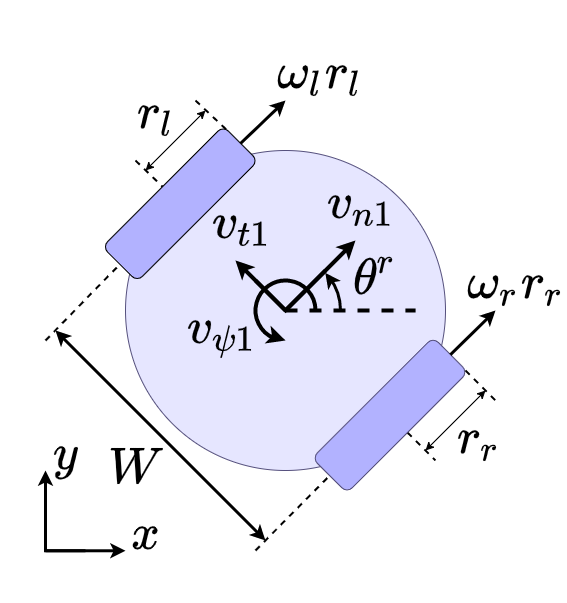
\includegraphics[width=0.8\textwidth]{figures/schematic_differential_drive_robot.png}
    \caption{Schematic 2D diagram of differential drive robot in world frame $<x, y, \theta>$, the robots frame's origin is located at $(x^r, y^r, \theta^r)$ and denoted as $<n1, t1, \psi1>$. The robot frames origin is where the robot's center of mass is located. The robot's left wheel has radius $r_l$, the right wheel has radius $r_r$, the robot wheels act upon the ground in the center of the wheel. The distance between where the left and right act upon the ground is notated as $W$. The angular speed of the left and right wheels are denoted by $\omega_l$ and $\omega_r$ respectively.}
    \label{fig: 2D_representation_robot}
\end{subfigure}%
\begin{subfigure}{.5\textwidth}
  \centering
 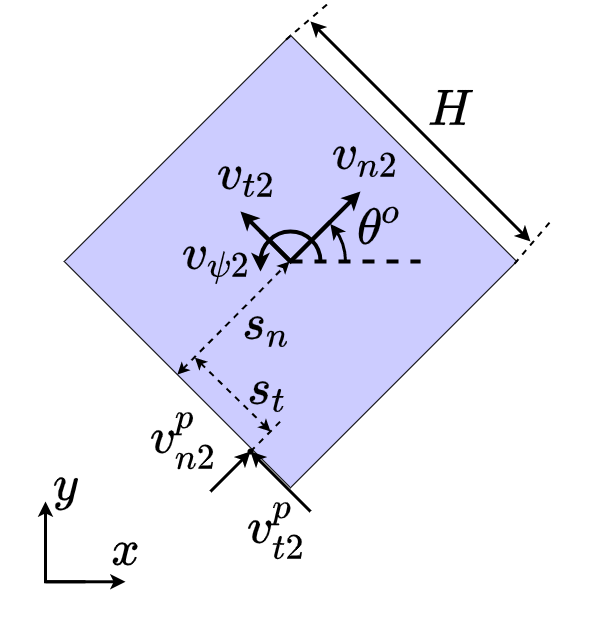
\includegraphics[width=0.8\textwidth]{figures/schematic_square_object.png}
    \caption{Schematic 2D diagram of cube object in world frame $<x, y, \theta>$, the object frame's origin is located at $(x^o, y^o, \theta^o)$ and denoted as $<n2, t2, \psi2>$. The object frames origin is where the cube's center of mass is located. Both length and width of the cube are $H$. A contact point $p$ is located at $s$ which can be decomposed in $s_n$ and $s_t$. An outside force pushes against at point $p$ the cube resulting in velocity component $v^p$ which can be decomposed in $v_{n2}^p$ and $v_{t2}^p$.}
    \label{fig: 2D_representation_object}
\end{subfigure}
\caption{Two example of single bodies}
\label{fig: single_body_models}
\end{figure}

let's consider an example system model, a differential drive mobile robot displayed in \cref{fig: 2D_representation_robot}. During design and construction, the robot can be fully analysed. When given the task to model the differential drive robot, it is thus reasonable to assume that some prior knowledge about the robot is known (e.g. weight or relation between forward velocity $v_{n1}$, wheel radiuses $r_l$, $r_r$, angular speeds $\omega_l$ and $\omega_r$). In that case, selecting and designing a \textit{differential equation} or \textit{parameterisable differential} equation is a logical option for reasons which will be discussed in  \cref{subsection: analytical_models,subsection: hybrid_models}. Literature reveals that a differential equation is a popular option to model a system \cite{bauza_data-efficient_2018, seegmiller_vehicle_2013}. Robots can come across a variety of objects, such as the cube object displayed in \cref{fig: 2D_representation_object}, both the differential drive robot and the cube object are modelled as differential equations displayed by \cref{equation: differential_equation_differential_robot} and \cref{equation: differential_equation_square_object} respectively.

\begin{equation}
\dot{\rho}^r(t)
=
\left[\begin{array}{l}
\dot{x}^r(t) \\
\dot{y}^r(t) \\
\dot{\theta}^r(t)
\end{array}\right]
=
f(\rho^r(t), u^r(t))
=
\left[\begin{array}{cc}
\cos (\theta^r(t)) & 0 \\
\sin (\theta^r(t)) & 0 \\
0 & 1
\end{array}\right]\left[\begin{array}{cc}
\frac{r_{l}}{2} & \frac{r_{r}}{2} \\
-\frac{r_{l}}{W} & \frac{r_{r}}{W}
\end{array}\right]\left[\begin{array}{l}
\omega_{l}(t) \\
\omega_{r}(t)
\end{array}\right]
\label{equation: differential_equation_differential_robot}
\end{equation}

\noindent With states $\rho^r(t) = \left[x^r(t) \quad y^r(t) \quad \theta^r(t)\right]^\top$, input $u^r(t)=\left[\omega_l(t) \quad \omega_r(t) \right]^\top$\\and constants $W$, $r_l$, $r_r$, $ > 0$. \Cref{equation: differential_equation_differential_robot}  from \cite{seegmiller_vehicle_2013}.\\

\Cref{equation: differential_equation_differential_robot} displays an analytical single-body model, if the equation would be expressed in robot frame it would be more compact because the transformation matrix (matrix containing both $\text{cos}(\theta^r(t))$ and $\text{sin}(\theta^r(t))$) is then scrapped, and instead of 3 state variables only two are sufficient. Later on, the two single bodies will be combined to one multi-body model, expressed in a world frame. For consistency, all system models accompanying the robot and cube example are in world frame.\\

\Cref{equation: differential_equation_square_object}  estimates the true dynamics of the cube object, because $v^p_{n2}$ acts upon the object, the object will translate and rotate. if the speed acts on the cube at the middle $s_t = 0$ then the speed will completely go to translation of the cube $v_{n2} = v^p_{n2}$. If the speeds acts on the cube at the corner $s_t = \pm \frac{H}{2}$, then the speed will completely go-to rotation of the cube, $\theta^o = v^p_{n2}s_t$. Linear interpolation between the middle and the corner points determines the ratio between translation and rotation, which is a function of speed $v^p_{n2}$  described as:

$$\dot{\theta}^o = \frac{2 s_t}{H} |s_t| v_{n2}^p$$
$$v_{n2} = (1-|\frac{2 s_t}{H}|) v_{n2}^p$$

yielding the following differential equation:

\begin{equation}
\dot{\rho}^o(t)
=
\left[\begin{array}{l}
\dot{x}^o(t) \\
\dot{y}^o(t) \\
\dot{\theta}^o(t)
\end{array}\right]
=
f(\rho^o(t), u^o(t))
=
\left[\begin{array}{c}
(1-|\frac{2 s_t}{H}|) \cos (\theta^o(t))v^p_{n2} \\
(1-|\frac{2 s_t}{H}|) \sin (\theta^o(t))v^p_{n2} \\
\frac{2 s_t}{H}|s_t|v^p_{n2}
\end{array}\right]
\label{equation: differential_equation_square_object}
\end{equation}

\noindent With states $\rho^o(t) = \left[x^o(t) \quad y^o(t) \quad \theta^o(t)\right]^\top$, input $u^o(t)=\left[v^p_{n2} \quad s_t\right]^\top $ \\and constant $H > 0$ and constraint $|s_t| \leq \frac{H}{2}$. \Cref{equation: differential_equation_square_object} is inspired by the analytical model in \cite{bauza_data-efficient_2018}.\\

\Cref{equation: differential_equation_square_object} is not approximating the true dynamics accurately, because pushing a cube using this differential equation does not capture any speed in the direction of the $t$-axis at point $p$. There is no friction of the object with the ground, let alone a distinction between static and dynamic friction which both affect the dynamics considerably. Simplifying the true dynamics results is model mismatch, too much simplification would eventually lead to a nonsense model, incapable of modelling the system behaviour accurately and leading to stability issues when used by a controller. \Cref{equation: differential_equation_square_object} simplifies too much and is thus an ineffective modelling method. However, for the purpose of an example \cref{equation: differential_equation_square_object} is sufficient. To improve modelling the true dynamics of a robot pushing a box, more details of the true dynamics should be captured. \cite{bauza_data-efficient_2018} created an analytical model for push manipulation involving Coulomb friction, force and friction constraints, resulting in a model modelled accurate enough to successfully track a reference signal. \cite{bauza_data-efficient_2018} performed a close inspection of the object to push. Assuming prior knowledge about the object to encounter is unrealistic as opposed to robot dynamics. Now the two single-body models will be combined as a multi-body model, a schematic 2D diagram is displayed in \cref{fig: multiple_body_diagram}. \\

\begin{figure}[H]
    \centering
    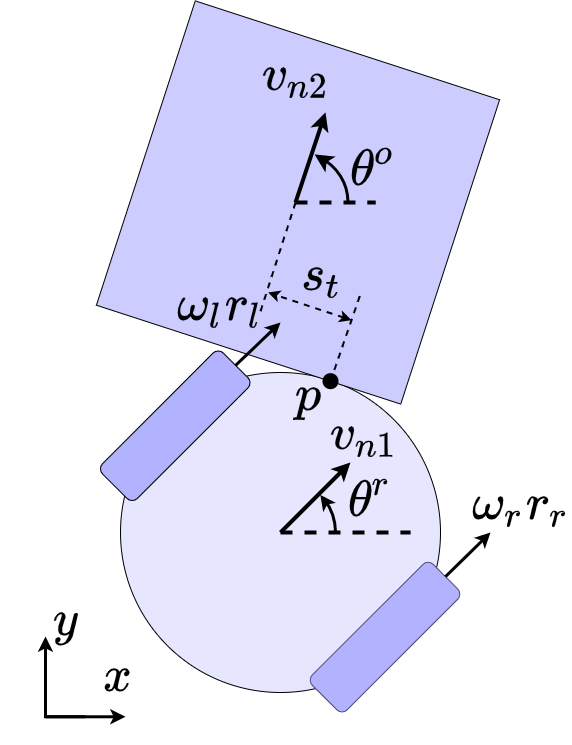
\includegraphics[width=0.38\textwidth]{figures/schematic_diff_drive_and_square.png}
    \caption{Combining single bodies \cref{fig: 2D_representation_robot,fig: 2D_representation_object} which are connected at contact point $p$ to create a multi body.}
    \label{fig: multiple_body_diagram}
\end{figure}

Augmenting the differential \cref{equation: differential_equation_differential_robot} with \cref{equation: differential_equation_square_object} creates a multi-body model:

\begin{equ}[H]
\begin{align}
\label{equation: multiple_body_model_robot_cube}
\dot{\rho}^{ro}(t)
&=
\left[\begin{array}{l}
\dot{x}^r(t) \\
\dot{y}^r(t) \\
\dot{\theta}^r(t) \\
\dot{x}^o(t) \\
\dot{y}^o(t) \\
\dot{\theta}^o(t)
\end{array}\right]
=
f(\rho^{ro}(t), u^r(t))\\ 
&=
\left[\begin{array}{ccc}
\cos(\theta^r(t)) & 0 & 0\\
\sin(\theta^r(t)) & 0 & 0\\
0 & 1 & 0 \\
0 & 0 & (1-|\frac{2 s_t}{H}|) \cos (\theta^o(t)) \\
0 & 0 & (1-|\frac{2 s_t}{H}|) \sin (\theta^o(t))\\
0 & 0 & \frac{2 s_t}{H}|s_t|
\end{array}\right]
\left[\begin{array}{cccc}
1& 0 \\
0 & 1 \\
cos(\theta^r(t) - \theta^o(t)) & 0 \\
\end{array}\right]
\left[\begin{array}{cc}
\frac{r_{l}}{2} & \frac{r_{r}}{2} \\
-\frac{r_{l}}{W} & \frac{r_{r}}{W}\\
\end{array}\right]
\left[\begin{array}{l}
\omega_{l}(t) \\
\omega_{r}(t) \\
\end{array}\right] \nonumber
\end{align}
\caption*{Combining both single-body models displayed in \cref{equation: differential_equation_differential_robot,equation: differential_equation_square_object} to obtain a multi-body model.}
\end{equ}

with $s_t$ now dependent on both the location and geometric properties of the robot and the object, defined as:

$$
s_t = \sqrt{(x^o(t)-x^r(t)-\frac{H+W}{2}cos(\theta^o(t)))^2 + (y^o(t)-y^r(t)-\frac{H+W}{2}sin(\theta^o(t))^2}
$$

The multi-body model in \cref{equation: multiple_body_model_robot_cube} displays how the first derivative of state variables can be calculated based on the input $u^r(t) = \left[\omega_l \quad \omega_r \right]$, the system constants $H$, $r_l$, $r_r$, $W$ and the state variables. The multi-body model estimates the true dynamics of the robot and the box. The robot and cube object are touching at point $p$, when the objects become disjoint the multi-object model is not a valid representation of the true dynamics any more. \\

This concludes the example of multiple single-body models into a multi-body model. In the example, we saw one way of analytically modelling a robot and an cube object. There is however a vast literature of different methods which could been applied to model \cref{fig: multiple_body_diagram} \cite{nascimento_nonholonomic_2018}, \cite{bauza_data-efficient_2018}, \cite{stuber_feature-based_2018}, \cite{stuber_lets_2020}. An overview of modelling methods reviewed is conveniently condensed into \cref{mindmap: classify_system_models}. Now the distinction between single-body models and multi-body models is clear, and the advantages and disadvantages per class of models are discussed.

\begin{figure}[h]
\centering
\resizebox{!}{11cm}{%
\begin{tikzpicture}[
    mindmap,
    concept color = myDarkColor,
    every node/.style = {concept},
    grow cyclic,
    level 1/.append style = {
        concept color = myLightColor,
        level distance = 4.4cm,
        sibling angle = 120
    },
    level 2/.append style =  {
        concept color = myEvenLighterColor,
        level distance = 2.8cm,
        sibling angle = 70
    }
]
\node  {System Model Classes}
    child {node {Analytical Models}
        child{node {State-Space Models}}
        child{node {Transfer Functions}}
        child{node {Dynamical Equation}}
    }
    child {node {Hybrid Models}
        child{node {Paramet- erisable Difference Models}}
    }
    child {node {Data-driven Models}
        child{node {Long Short-Term Memory}}
        child{node {Gaussian Distribution Estimation}}
        child{node {Contact Models}}
    };
\end{tikzpicture}
}
\caption{A mind map showing the classification of different system models representations investigated in this literature. The first level of children displays the model classes, the second level displays examples of the model classes, classification \cite{stuber_lets_2020}.}
\label{mindmap: classify_system_models}
\end{figure}

\subsection{Analytical models}
\label{subsection: analytical_models}
Historically, analytical models are the first models to emerge, most prominently used are \textit{state-space} representations, \textit{transfer functions} and \textit{differential equations}. Building an analytical model requires thorough knowledge of the system it models, because every system parameter, such as mass, damping coefficient, the center of gravity, geometry, friction coefficient or inertia. Analytical approaches rely on accurate identification of physical parameters which makes analytical models unfit for manipulation while learning system models \cite{arruda_uncertainty_2017}, \cite{stuber_feature-based_2018}.\\

Nevertheless, the work in \cite{bauza_data-efficient_2018} manages to create a stable controller for push manipulation using an analytical model. Because thorough model identification of the pushable object was performed, the trajectory error stayed within reasonable boundaries. 

\subsection{Data-driven models}
\label{subsection: data_driven_models}
Among recent studies, data-driven models shown an uptrend in popularity \cite{mericli_push-manipulation_2015},
\cite{bauza_data-efficient_2018},  \cite{stuber_feature-based_2018}, \cite{stuber_lets_2020}. Fully data-driven methods don't model any structure of the system it describes, or use a generalised model which applies to all. A system is viewed as a black box, which is fed input and gives back output. This reduces the need for prior information about the system significantly. \ac{IO} data is analysed to estimate the structure of the black box. The \ac{IO} data analysed which solemnly serves the creation of a model is called the \textit{model train set}. The advantage of requiring a minimum of prior information comes at the cost of the amount of \ac{IO} data required. If there is not sufficiently much data, or the data is not rich enough then the model will not be accurate. For example, \cite{bauza_data-efficient_2018} compared a purely analytical approach with a data-driven approach in push manipulation. The data-driven approach can take up to 200 samples of \ac{IO} data to sufficiently match the performance of an analytical controller. With more \ac{IO} data, data-driven approaches lower output errors and increase performance, outperforming analytical approaches but also outperforming hybrid approaches, which are discussed in the next subsection. Data-driven approaches outperform because data-driven approaches capture even tiny dynamical details of the true dynamics. That is, assuming that the dynamical details reside in the \ac{IO} data. \\

A field of research which has become very popular in recent years is artificial intelligence. In for example, estimating physical parameters from data. This is what \cite{denil_learning_2017} has shown with the use of deep reinforcement learning. By learning physical parameters artificial intelligence can help tackle the main issue with analytical approaches, estimating physical parameters. Instead of explicitly estimating physical parameters, another approach is learning a dynamics model directly \cite{stuber_lets_2020}. \cite{cong_self-adapting_2020} showed a powerful self-adapting push controller based on a \textit{long short-term memory} modelling approach. A powerful advantage is online adaptation, which lowers a time-consuming train set to a warm start of approximately 5 test pushes with an object to push. \\

Alternatively, a set of robot-object test pushes can be used to fit a underlying distribution. Where test pushes and their effect on the object's position and velocity are taken as a train set, then a distribution is fitted mapping the train set's input to it's output. Such an fitted distribution is called a \textit{contact model}. Recent literature shows a \textit{Gaussian distribution} is a popular distribution used by \cite{mericli_push-manipulation_2015} and \cite{stuber_feature-based_2018}. \cite{stuber_feature-based_2018} includes, additionally to a robot-object model (fitted from test pushes) an object-environment model, which considers object surface features. Object-environment information is added by modelling the surfaces of an object. All objects have surfaces, from a simple cube with 6 equal surfaces to more complex shapes. For the object-environment contact model, a central aspect is the probabilistic modelling of surface features, which describes every surface as a 3D position, 3D orientation and 2D local surface descriptor that encodes local curvatures. The data stored for surface features come from 3D point clouds created with a depth camera. An advantage is that the object environment model can be constructed based on 3D point cloud, and no interaction with the object is required. After having learned the contact model (object-environment model), a robot-object motion model is learned for which test pushes are required \cite{stuber_feature-based_2018}. \\

Contact models used for push manipulation make use of robot-object contact or additionally use object-environment contact. With enough rich data contact models outperform analytical and hybrid approaches. To tackle the amount of data required a more hybrid approach is developed. Which separates agent-object contact from object-environment contact. To generate a new model, two things are required, first an object-environment contact model of the object to model, and second, a sufficiently learned agent-object contact model. The latter does not necessarily have to be created from the object to model, existing agent-object contact models, combined with transfer learning can be sufficient \cite{kopicki_learning_2017}. \\

The nonlinear effects which dominate multi-object system resides in \ac{IO} data, because data-driven approaches models are not assuming any structure which could limits capturing nonlinear effects, the data-driven approaches are a worthy method for estimating true dynamics of in particular multi-body systems. It must be mentioned that data-driven methods outperform other model classes with enough data, for which the training time is in robotics not always available. If other modelling approaches are available which estimating true dynamics accurate enough, the data-driven approach should be avoided because of the long lasting training time.  

\subsection{Hybrid models}
\label{subsection: hybrid_models}
Hybrid models are an extension of analytical approaches with data-driven methods. Whilst the interactions between objects are still represented analytically, some quantities of interest are estimated based on observations (e.g. the coefficients of friction) \cite{stuber_lets_2020}. Recent literature reveals the foremost hybrid methods are parameterisable differential equations. Parameterisable state-space models and parameterisable transfer models do exist, though the most widely used parameterisable model remains a parameterisable differential model, which takes the form:
\begin{equation}
   \frac{dx}{dt}=f(x, u, p) 
   \label{equation: parameterisable_model}
\end{equation}

where $x$ is the state vector, $u$ is the input vector and $p$ is the parameterisation which needs to be found such that $f(x,u,p)$ accurately estimates the true dynamics. With a random or educated initial guess of the parameterisation $p$, a system model is provided without full knowledge of all system parameters. An example parameterisation for analytical model example \cref{equation: differential_equation_differential_robot}.

% would be $p = \begin{bmatrix} r_l & \r_r & W\end{bmatrix}^\top$.

An initial guess as parameterisation may not be a very accurate model, but it does allow to skip a tedious system identification period. Online adaptation allows to converge to a local minimum during execution. Whether this local minimum also coincides with the global minimum is dependent on the optimisation technique and the initial guess. Parameterisable differential models are very powerful in situations where the general structure of dynamics is known, but certain parameters e.g. weight, the friction coefficient is unknown or change over time \cite{seegmiller_vehicle_2013}.\\

Single-bodies can and should be modelled as hybrid models, hybrid models allow a workable model which can be created from only the prior structural knowledge of the system. After some off or online system identification detailed parameters can be found, as effect the model will converge toward the true dynamics. While data-driven methods outperforms hybrid methods such methods take long to properly train. Multi-body models are dominated by nonlinear dynamics, to fully capture such nonlinear dynamics, data-driven methods can and should model multi-body model, even if this means collecting a large train set. 

In a environment with unknown objects, the ability to rapidly interact with objects is provided by hybrid models. During interaction hybrid approaches can improve their model accuracy whilst also adapting to changing systems. To fully capture the push mechanics, data-driven methods should be used, because only data-driven methods are able to capture a large portion of the nonlinear dynamics.


% Answers the question:
% What are methods to learn dynamic models and what are the limitations

% connecting to motion planning by adding dynamic constraints to a planner in configuration space. 
\section{Interaction Approaches and Model Identification Methods}
\label{section: interaction_approaches_and_model_iden_methods}
% introduce most prominent types of controllers
This section will describe the most prominent control methods which are applicable for controlling single- or multi-bodies. In general controllers have 3 abilities, which are tracking a reference signal, stabilising a system or rejecting disturbances, a controller can focus on one or a combination of these 3 abilities. The controllers' goal in this literature lies in tracking a reference signal to lower the output error. In \cref{section: system_model_representation} single-body models and multi-body models were introduced, now their control versions are introduced. \textbf{Single-body control} is an interaction approach which learns a single-body model and controls a single-body. As a reminder, a single-body is an object which is assumed to be connected for all times. \textbf{Multi-body control} controls two or more single- or multi- bodies. A multi-body controller uses a multi-body model. For example, a mobile robot pushing a ball. A controller actuates the robot directly and the object indirectly via the robot. Another example is a controller actuating a robot arm with a gripper holding a box. Single-body control involves driving for mobile robots and moving for a fixed robot. Multi-body control involves the robot pushing an object. The ability to push greatly broadens the robot's capabilities. Objects which are too heavy to lift could potentially still be pushed, objects out of reach to grasp could be in reach to push, and a gripper holding an object can additionally push another object but cannot grasp two objects at the same time.\\

Existing literature presents several methods for model-based robot control. The most prominent and established techniques can be categorised as predictive methods such as \ac{MPC} and reactive methods such as \ac{PID} control. Literature shows 2 types of model-free methods, completely model-free methods which act directly on \ac{IO} data, and model-free methods which are provided with data, but not explicitly given any model. Such   methods service by analysing \ac{IO} data and using system identification to update a model, whilst a controller uses such a model simultaneously.\\

Extensive research on robot controllers from last decades has been categorised in \cref{mindmap: classify_controllers}. \Cref{table: summary_controllers} provides a more detailed overview of some interaction approaches. 

\begin{figure}[ht]
\label{mindmap: classify_controllers}
\centering
\resizebox{!}{11cm}{%
\begin{tikzpicture}[
        mindmap,
    concept color = myDarkColor,
    every node/.style = {concept},
    grow cyclic,
    level 1/.append style = {
        concept color = myLightColor,
        level distance = 4.4cm,
        % sibling angle = 120
    },
    level 2/.append style =  {
        concept color = myEvenLighterColor,
        level distance = 2.8cm,
        % sibling angle = 100
    }
]
\node  {Controller Classes}
    child [grow = 310]{node {Predictive Methods}
        child[grow=300]{node {\ac{MPC}}}
        child[grow=240]{node {\acs{MPPI}}}
    }
    child [grow = 0]{node {Intelligent methods}
        child[grow=30]{node {\scriptsize \hspace{-0.2cm} \shortstack[]{ Reinforcement\\Learning}}}
        child[grow=330]{node {\acs{LSTM}}}
    }
    child [grow = 230]{node {Reactive methods}
        child[grow=300]{node {\ac{PID}}}
        child[grow=240]{node {Active Inference}}
    };
\end{tikzpicture}
}
\caption{A mind map showing the classification of control methods investigated in this literature. The first level of children displays the control classes, and the second level displays examples of the control classes \cite{mehra_map_2022}}
\end{figure}


% discuss all PID related papers
\subsection{Reactive Methods}
\label{subsection: reactive_methods}
Historically reactive methods were the first to arise. A widely used control method is the \ac{PID} controller. It's widely used due to its simplicity, clear functionality and ease of implementation. Tuning a \ac{PID} controller can be split up into 3 tuning approaches. Heuristic-tuning, rule-based tuning and model-based tuning \cite{tools_explore_2022}. A heuristic tuning method is one where general rules are followed to obtain approximate or qualitative results. The trial-and-error method is an example of heuristic tuning. Heuristic tuning is a quick and easy method to obtain a reasonable result, finding good performance can be very time-consuming. Rule-based \ac{PID} tuning methods assume a certain process response to obtain easy mathematical formulas that enable the tuning of a \ac{PID} controller. Commonly used rule-based tuning methods are the Ziegler-Nichols, Chien, Hrones and Reswick tuning methods. Performance improves and some stability guarantees arise, however for rule-based tuning some prior process knowledge is required. Model-based tuning or optimization-based \ac{PID} tuning allows you to obtain your P, I, and D parameters optimally. Control objectives such as disturbance rejection and reference tracking together with a model of your system and the engineering specifications of the closed-loop behaviour determine the final set of tuning parameters. Optimal performance comes at the cost of full prior system knowledge. For single-object control, the heuristic and rule-based tuning methods can apply because for these tuning methods full system knowledge is not required. For multi-body control, only the heuristic method could apply. In recent years automatically tuning \ac{PID} gains with more complex methods has risen. Such as \cite{ahn_online_2009} showed, who tuned a \ac{PID} controller using fuzzy logic this shows reactive control methods can be used without the need for extensive prior knowledge of the system. \\

\ac{PID} control has been around for many years. As opposed to this classical approach, the active Inference (AI) controller has been developed in the last decade and finds its origin in the field of neuroscience. Neuroscientist Karl Friston combined action selection with \ac{PEM}, which created the free-energy principle \cite{friston_free-energy_2009}, \cite{friston_action_2010}. In the field of robotics, \cite{pezzato_novel_2020} proposed an AI controller and implemented it on a real system for the first time. The AI controller is implemented on a real system. The control approach is a model-free online joint space controller, which was implemented on a 7-DOF Panda robot arm. The controller adapted rapidly to a changing environment and accounted for additional Gaussian noise for the joint measurements. If the free-energy depends explicitly on the control actions, then AI can provide a excellent fault metric as \cite{baioumy_fault-tolerant_2021} and \cite{pezzato_active_2021} have shown. One of the current drawbacks with an AI controller, there does not yet exist a stability proof and the solution to which the controller converges might be a local minimum. 
 
% discuss all MPC related papers
\subsection{Predictive Methods}
\label{subsection: predictive_methods}
In recent literature involving predictive methods \acf{MPC} methods are dominating, before moving on to \ac{MPC} and variations of \ac{MPC}, \ac{MPC} will briefly be explained.  The basic concept of \ac{MPC} is to use a dynamic model to forecast system behaviour and optimise the forecast to produce the best decision for the control move at the current time. Models are therefore central to every form of \ac{MPC}. Because the optimal control move depends on the initial state of the dynamic system\cite{rawlings_model_2020}. A dynamical model can be presented in various forms, let's consider a familiar differential equation. 
$$ \frac{dx}{dt} = f(x(t), u(t)) $$
$$ y = h(x(t), u(t)) $$ 
$$ x(t_0) = x_0 $$

In which $x \in \mathbb{R}^n $ is the state, $u \in \mathbb{R}^m$ is the input, $y \in \mathbb{R}^p$ is the output, and $t \in \mathbb{R}$ is time. The initial condition specifies the value of the state $x$ at $t = t_0$, and a solution to the differential equation for time greater than $t_0$, $t \in \mathbb{R}_{\geq 0}$ is sought. If little knowledge about the internal structure of a system is available, it may be convenient to take another approach where the state is suppressed, no internal structure about the system is known and the focus lies only on the manipulable inputs and measurable outputs. As shown in \cref{figure: mpc_block_diagam}, consider the system $G(t)$ to be
the connection between $u$ and $y$. In this viewpoint, various system identification techniques are used, in which $u$ is manipulated and $y$ is measured \cite{rawlings_model_2020}. From the input-output relation, a system model is estimated or improved. The system model can be seen inside the \ac{MPC} controller block in \cref{figure: mpc_block_diagam}.\\

\begin{figure}[h]
\centering
\begin{tikzpicture}
% blocks
\node[draw,
    minimum width=2cm,
    minimum height=1.2cm,
    fill=myLightColor,
] (system) at (0,0){$G(t)$};
\node[draw,
    minimum width=5.5cm,
    minimum height=2cm,
    fill=myEvenLighterColor,
    below = 1cm of system,
    label=above:MPC controller,
] (controller) {};
% the blocks and arrows inside MPC
\node[draw, minimum width=2cm, below=3mm of controller.north, anchor=north, fill=myDarkColor] (optimisation) {Optimisation};
\node[draw, below=8mm of optimisation.south, anchor=south, fill=myDarkColor] (model) {System Model};
\path[-stealth]
        (model.east) edge[bend right=70] node[pos=0.5, right] {Predict} (optimisation.east)
        (optimisation.west) edge[bend right=70] node[pos=0.5, left] {Action}  (model.west);
% Arrows
\draw[-stealth] (controller.west) |- ($(controller.west) - (1,0mm) $) |- (system.west) 
node[near end, above]{$u(t)$};
\draw[stealth-] ([yshift=-0.3cm]controller.east) -- ++(3,0) node[midway, above](input){$y_{ref}(t)$, $p$, $\mathbb{X}$, $\mathbb{U}$, $\mathbb{Y}$};
\draw[-stealth] (system.east) -- ++ (5, 0) 
    node[midway](output){}node[midway,above]{$y(t)$};
    \draw [-stealth] (output.center) |- ([yshift=0.5cm]controller.east); 
\end{tikzpicture}
\caption{System $G(t)$ with input ${u}(t)$, output $y(t)$ and \acs{MPC} controller with input $y(t)$, reference signal $y_{ref}(t)$, parameterisation $p$ and constraint sets $\mathbb{X}$, $\mathbb{U}$, $\mathbb{Y}$} \label{figure: mpc_block_diagam} \end{figure}  

As indicated in the problem description in \cref{section: problem_description}, prior knowledge about the structure of the robot itself is known. Such structure can be specified in a parameterisable system model, in which the influence of inputs and current states describes the behaviour of states and outputs. Uncertain parameters have to be sought, such as the center of mass, mass, and diameter of wheels. These parameters reside in the parameterisation $p$, see \cref{equation: parameterisable_model}. \Cref{figure: mpc_block_diagam} shows the parameterisation $p$, for purely analytical system models the parameterisation is left empty. The following explanation about \ac{MPC} is best understood with the differential drive robot in mind from \cref{fig: 2D_representation_robot}, with single-body model \cref{equation: differential_equation_differential_robot}. Some states of the system might be inside an obstacle region, such a region is undesirable for the robot to be in or go toward. The robot states are allowed in free space, which is all space minus the obstacle region. The free space is specified as a state constrained set $\mathbb{X}$. Allowable input can be restricted by the input constraint set $\mathbb{U}$, a scenario in which input constraints are required is for example the maximum torque an engine produces at full throttle. Lastly, the set of allowed outputs is specified in the output constraint set $\mathbb{Y}$. State, input and output constraints must be respected during optimisation, the optimiser takes the state-, input- and output constraint sets $\mathbb{X}$, $\mathbb{U}$, $\mathbb{Y}$ and if feasible, finds an action sequence driving the system toward the reference signal while constraints are respected. The \ac{MPC} system model predicts future states where the system is steered toward as a result of input actions.\\

The optimisation minimises an objective function $V_{N}(x_{0}, y_{ref}, \mathbf{u}_{N}(0))$, where\\ $ \mathbf{u}_{N}(k) = (u_k, u_{k+1}, \dots , u_{k+N})$. The objective function takes the reference signal as an argument together with the initial state and the control input for the control horizon. The objective function then creates a weighted sum of some heuristic function. States and inputs resulting in outputs far from the reference signal are penalised more by the heuristic function than outputs closer to the reference signal. Because the objective function is a Lyapunov function, it has the property that, it has a global minimum for the optimal input $\mathbf{u}_{N}^*$. If the system output reaches the reference signal $y_{ref}$, $x_{ref}$ then $u_{ref}$ will be mapped to the output reference signal as such $y_{ref} = h(x_{ref}, u_{ref})$. As a result solving the minimisation problem displayed in \cref{equation: mpc_problem} gives the optimal input which steers the system toward the output reference signal while at the same time respecting the constraints. 


\begin{mini}
{u_k, u_{k+1}, \dots , u_{k+N}} {
V_{N}(x_{0}, y_{ref}, u_k, u_{k+1}, \dots , u_{k+N})
}
{}{}
\addConstraint{x(k+1) = f(x(k), u(k))}
\addConstraint{x \in \mathbb{X}}
\addConstraint{u \in \mathbb{U}}
\addConstraint{y \in \mathbb{Y}}
\addConstraint{x(0) = x_0}
\label{equation: mpc_problem}
\end{mini}

\Cref{figure: mpc_scheme_basic} displays the predicted output converging toward the constant output reference. After solving the minimisation problem, \cref{equation: mpc_problem}, the optimal input sequence is obtained $\mathbf{u}^*_N$ (given that the constraints are respected for such input), from which only the first input is executed for time step $k$ to $k+1$. Then all indices are shifted such that the previous time step $k+1$ becomes $k$, the output is measured and the reference signal, parameterisation, and constraints sets are updated and a new minimisation problem is created, which completes the cycle. Note that \cref{figure: mpc_block_diagam,figure: mpc_scheme_basic} is an example \ac{MPC} controller, which hardly scratched the surface of \ac{MPC}, there are many variations and additions such as deterministic and stochastic \ac{MPC}, stage and terminal cost, distributed \ac{MPC}, etc. which \cite{rawlings_model_2020} visits extensively. 

\begin{figure}[h]
    \centering
    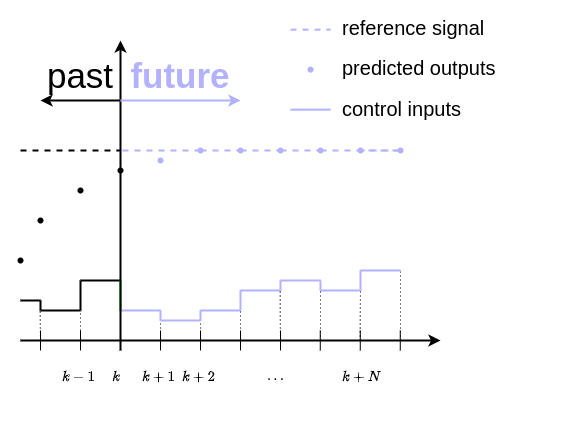
\includegraphics[width=0.8\textwidth]{figures/MPC_simple_diagram.png}
    \caption{A discrete \acs{MPC} scheme tracking a constant reference signal. $k$ indicates the discrete time step, $N$ the control horizon}
    \label{figure: mpc_scheme_basic}
\end{figure}

A major flaw for \ac{MPC} was the computation time required to solve a minimisation problem every time step. Because processors' power has increased, the \ac{MPC} framework can be applied in real time and is applicable for robotics. When applied to tracking a reference signal the \ac{MPC} framework outperforms classic control approaches such as \ac{PID} control \cite{nascimento_nonholonomic_2018}. Where \ac{MPC} excels at is tracking multiple objectives which can be weighted in the objective function. For example, \ac{MPC} can primarily track a robot path, while secondarily satisfying some additional dynamic specifications. This makes \ac{MPC} especially suitable in path tracking for nonholonomic robots. By restricting the state constraint set, obstacles can be avoided, such obstacles can even be avoided online  because the state constraint set may be changed during execution. It should however be feasible to find an input which satisfies all constraints. Because of its ease of tuning, handling multiple objectives, and flexibility in adding constraints, \ac{MPC} became the baseline standard to compare new control approaches with in control research. By now, linear \ac{MPC} theory is quite mature, and important issues
such as stability are well addressed in the last decade. Nevertheless, some systems are, in general,
inherently nonlinear. Therefore, especially in highly dynamic systems such as mobile robotics, linear
models are often inadequate to describe the process dynamics and nonlinear models have to be used. Thus nonlinear \ac{MPC} theory is required for which closed-loop stability proofs are lacking \cite{nascimento_nonholonomic_2018}. \\

Now the reader has gained a basic understanding of the workings of \ac{MPC} let's see relevant literature in the context of robot control in an environment with unknown objects. Starting with the literature accompanying single-body control.

\subsubsection*{(Integrated) Prediction Error Minimisation}
As mentioned models are central in every form om \ac{MPC}, so obtaining models is very important. \Cref{figure: mpc_block_diagam} displays a system model inside the block diagram used by the \ac{MPC} controller. The \ac{MPC} framework is flexible in handling different types of models, it accepts analytical, data-driven or hybrid forms. The \ac{MPC} controller's performance heavily relies on the accuracy of the system model. Having an accurate system model is thus crucial in the \ac{MPC} framework. One major system identification technique is the \ac{PEM} approach, it is the core of black-box identification methods \cite{farina_convergence_2008}. Generally in \ac{PEM} methods, the objective is to determine, from a finite number of measurements of the input and output sequences, a one-step-ahead predictor without prior system knowledge, or the system and covariance matrices of stochastic disturbances. The creation of an estimated model yields a state-space model or a transfer function model from which predictions can be made. \cite{verhaegen_filtering_2007}. An example is used to further clarify \ac{PEM} methods.

\subsection{Example Identification Method}
\begin{figure}[h]
\centering
\begin{tikzpicture}
% H, G and State-Space blocks
\node[draw,
    minimum width=2cm,
    minimum height=1.2cm,
    fill=myLightColor,
] (H) at (0,0){$H(q)$};
\node[draw,
    minimum width=2cm,
    minimum height=1.2cm,
    fill=myLightColor,
    below left =1cm of H,
] (G) {$G(q)$};
\node[draw,
    minimum width=3.5cm,
    minimum height=2cm,
    fill=myEvenLighterColor,
    below left= 1cm and -3.5cm of G,
] (SS) {\shortstack[l]{$A(p)$, $B(p)$, $K(p)$\\ $C(p)$, $D(p)$}};
%  two sum shapes
\node[draw, circle, minimum size=0.6cm, below= 1cm of H,] (sum) {};
\draw (sum.north east) -- (sum.south west)
    (sum.north west) -- (sum.south east);
\draw (sum.north east) -- (sum.south west)
(sum.north west) -- (sum.south east);
\node[left=-1pt] at (sum.center){\tiny $+$};
\node[above] at (sum.center){\tiny $+$};
\node[draw, circle, minimum size=0.6cm,below right= 0.4cm and 4cm of G] (pm) {};
\draw (pm.north west) -- (pm.south east);
\draw (pm.north east) -- (pm.south west)
(pm.north west) -- (pm.south east);
\node[above] at (pm.center){\tiny $-$};
\node[below] at (pm.center){\tiny $+$};
\draw[-stealth] (H.south) -| (sum.north);
\draw[-stealth] (G.east) -- (sum.west);
% every arrow 
\draw[-stealth] (sum.east) -| (pm.north)
node[midway](output){}node[midway,above]{$y(k)$};
\draw[-stealth] ($(output.center) - (1,0mm)$) |- ++(0,-1) -| ($([yshift=0.5cm]SS.west) - (1,0mm) $) -- ([yshift=0.5cm]SS.west);
\draw[stealth-] (G.west) -- ++(-3, 0)
node[](input){}node[midway, above]{$u(k)$};
\draw[-stealth] ($(input.center) + (1,0mm)$) |- ([yshift=-0.5cm]SS.west);
\draw[-stealth] (SS.east) -| (pm.south)
node[midway, below] {$\hat{y}(k, p)$};
\draw[-stealth] (pm.east) -- ++ (1,0)
node[near end, above] {$\epsilon(k,p)$};
\draw[stealth-] (H.west) -- ++ (-1,0) node[midway, above] {$e(k)$};
\end{tikzpicture}
\caption{A block diagram displaying the structure of the prediction-error model-estimation method \cite{verhaegen_filtering_2007}}
\label{figure: pem_block_diagram} \end{figure}  

\Cref{figure: pem_block_diagram} displays a block diagram of the prediction-error model-estimation method. Here output $y(k)$ is created by summing system $G(q)u(k)$ with additional noise $H(q)e(k)$, the input $u(t)$ is stochastically independent of $e(k)$ a zero-mean white-noise sequence. The one-step-ahead predictor tunes the state matrices $A(p)$, $B(p)$, $K(p)$, $C(p)$, $D(p)$ such that the output error $\epsilon(k,p)$ is minimised.

Two important assumptions are: $G(q)$ is an \ac{LTI} system, and the stationary one-step-ahead predictor displayed in \cref{equation: verhaegen_one_step_ahead} is of known order.
In this example the goal is to obtain the state-space matrices from input-output data. \Cref{figure: pem_block_diagram} displays a block diagram of the \ac{PEM} methods. With input-output data generated as:

\begin{equ}[!ht]
\begin{equation}
y(k) = G(q)u(k) + H(q)e(k)
\label{equation: verhaegen_signal_generating}
\end{equation}
\caption*{A signal-generating system, it's input-output data is to be used for identification. $G(q)$ represents the deterministic part and $H(q)$ the stochastic part of the system, both $G(q)$ and $H(q)$ are discrete transfer function models, from \cite{verhaegen_filtering_2007}}
\end{equ}

The one-step-ahead predictor of known order takes, for a state-space model the following form:
\begin{equ}[!ht]
\begin{equation}
\begin{aligned}
\hat{x}(k+1) &=A \hat{x}(k)+B u(k)+K(y(k)-C \hat{x}(k)-D u(k)), \\
\hat{y}(k) &=C \hat{x}(k)+D u(k)
\end{aligned}
\label{equation: verhaegen_one_step_ahead}
\end{equation}
\caption*{Given a finite number of samples of the input signal $u(k)$ and the output signal $y(k)$, and the order of the predictor. The goal is to estimate the system matrices $A$, $B$, $C$, $D$ and $K$ in this predictor such that the output $\hat{y}(k)$ approximates the output of \cref{equation: verhaegen_signal_generating}}
\end{equ}

A parameterisation of the one-step-ahead predictor as a stationary Kalman filter, \cref{equation: verhaegen_one_step_ahead} with parameterisation $p$ and the one-step-ahead predictor of the previous time step gives the parameterised one-step-ahead predictor:

\begin{align*}
\hat{x}(k+1|k, p) &= (A(p)-K(p)C(p))\hat{x}(k|k-1,p) + (B(p)-K(p)D(p))u(k) + K(p)y(k)\\ \hat{y}(k|k-1, p) &= C(p)\hat{x}(k|k-1, p)  + D(p)u(k)
\end{align*}

By minimising the output error $y(k) - \hat{y}(k|k-1,p)$ an optimal parameterisation is be found, such a parameterisation together with its parameterisable one-step-ahead predictor can be used by the \ac{MPC} framework. Chapter 8, \cite{verhaegen_filtering_2007} can elaborate further on \ac{PEM} methods with subjects such as the ARMAX, ARX and Box-Jenkins parameterisation, the innovation model or closed-loop system behaviour. \ac{PEM} system identification techniques rely on \ac{IO} data, which must contain enough information, which in robotics can be an issue, since there is not always time to collect a rich enough \ac{IO} data set. Though, \ac{PEM} methods can with little prior knowledge formulate an accurate system model, if provided with enough \ac{IO} data. \cite{farina_convergence_2008} has compared single- and multistep \ac{PEM} methods and convergence properties in a predictive control context, and provided proof that showing that single step and multistep \ac{PEM} methods yield unbiased models. This allows the conclusion that \ac{PEM} methods are proper methods to estimate a linear system model, provided that there is access to enough information-rich \ac{IO} data of such a system. \ac{PEM} assumes the true dynamics can be estimated accurately with an \ac{LTI} system, \ac{PEM} methods are ideal for single-body control. \ac{PEM} for multi-body control is feasible, but not ideal since multi-body control is too nonlinear to be properly captured using an \ac{LTI}-based system identification method.\\

An improvement on \ac{PEM} which lacks capturing changing dynamics, was made by \cite{seegmiller_vehicle_2013} where a system model is parameterised using \ac{IPEM}. The idea is to integrate the left-hand side $\frac{dx}{dy}$ of the system dynamics, resulting in some favourable effects. \ac{IPEM} can calibrate offline (slip) and online (odometry), \ac{IPEM} improves upon \ac{PEM} by using only low-frequency measurements, and fewer ground truth measurements and slip can be accounted for. These plus points come at the cost of additional complexity.
Because fewer measurements are required, \ac{IPEM} detects and adjusts faster to changing system dynamics, which makes \ac{IPEM} more suitable for robotic applications compared to \ac{PEM}. Additionally \ac{PEM} assumes an \ac{LTI} system, where \ac{IPEM} claims to converge for a linear time-variant system, broadening the set of systems \ac{IPEM} can model. Especially for the following situation which is described in \cite{seegmiller_vehicle_2013}. A robot plans to make an aggressive turn into a narrow corridor, however, due to unmodeled understeering, the
robot actually makes a wider than expected turn driving into the wall of the corridor. The robot has deviated from the planned path. Based on position feedback, the robot
compensates by planning a sharper turn. Once again, the robot fails to execute the planned path as its curvature exceeds the limits
of the steering mechanism. The robot must now abandon the attempt and drive in reverse to avoid a collision. If the planner had an
accurate model, it would have simply turned harder at the beginning of the turn when the turn was still feasible.\\

\ac{IPEM} methods are ideal for estimating rapid-changing true dynamics with a stochastic nature, arising during tracking of a reference for a mobile robot with additional measurement noise. The mobile driving robot can be modelled as a linear time-variant model which accounts for slip and odometry changes.\\

\ac{PEM} and \ac{IPEM} are suitable for single-body models because single-body systems can be simplified to an \ac{LTI} system. Multi-body systems cannot since they are dominated by nonlinear dynamics. Multi-body system thus require a different system identification method, recent literature reveals that a set of test pushes is the dominant data collection method for gathering a set of \ac{IO} data. As the name "test pushes" suggests, data collection focuses on push manipulations and is collected by the robot performing several test pushes against the object from different angles. The push is taken as input, and the location of velocity of the object is taken as output to form a train set. From this train set, there exist multiple methods to create a system model. Let's review recent literature,  for every new object, \cite{mericli_push-manipulation_2015} creates, a sequence of random push actions and the effect of the push. A 3-dimensional Gaussian distribution (for 2D pose variables $x$, $y$ and $\theta$) is fitted on the sample pushes. The Gaussian distribution can be used as a one-step-ahead predictor used for control. A disadvantage of \cite{mericli_push-manipulation_2015} is, after every push the object comes to a complete stop. A sequence of pushes is generated and executed in a push-stop-push-stop fashion, which could be one continuous push. \cite{bauza_data-efficient_2018} overcomes this problem by converting the Gaussian process to linearized motion equations which can be directly fed into the \ac{MPC}. Both \cite{mericli_push-manipulation_2015} and \cite{bauza_data-efficient_2018} use data-driven approaches, \cite{bauza_data-efficient_2018} additionally has an analytical approach. Initially, an analytical approach has the lowest tracking error, after $\sim 100$ number of tests pushes the data-driven approaches outperform analytical approaches because the push analytical models does model the more nonlinear parts of the true dynamics. Such as small variations in the sliding friction or the mass distribution. \cite{bauza_data-efficient_2018} did show a data-driven stable controller can be created after only $\sim 10$ test pushes. \\  

In the \ac{MPC} frameworks, several single- and multi-body methods are discussed, transitioning from single-body control to multi-body control can causes problems. Single-body control requires the constraints which belong to a single-body model, when single-body control switches to multi-body control the dynamical and kinematic constraints should update such that the multi-body constraints are respected. This discontinuity of model dynamics introduces control and planning problems. Control issues arisen during discrete dynamic models are now discussed, the arisen problems affecting planning will be discussed in the next chapter.\\

\subsubsection*{Reactive \ac{MPC}}
As \cite{toussaint_sequence--constraints_2022} describes in their problem description: \ac{TAMP} plans include switches in kinematic and dynamic constraints, and the original plan might provide temporal scheduling of such switches. However, for reactive execution the exact timing of constraint switches needs to be reactive, which either requires employing optimization methods invariant to such switches \cite{toussaint_differentiable_2019}, \cite{posa_direct_2014} or include explicit timing-estimation and -optimization as part of the \ac{MPC} problem.\\

The solution proposed by \cite{toussaint_sequence--constraints_2022} is to take the timing of switching constraints as a decision variable yielding a timing-optimal sequence-of-constraints \ac{MPC}. Because the reactive \ac{MPC} can work with somewhat accurate system models, the reactive  \ac{MPC} controller is ideal for objects for which a not very accurate model of the true dynamics is only available. The reactive behaviour makes the control algorithm well suited for pushing and avoiding collision of incoming objects. A disadvantage in reactive \ac{MPC} is the CPU power it requires to run, another drawback is that a reactive \ac{MPC} is unable to learn any system model, the reactive controller cannot give any guarantees when operating on unknown objects. However, if a (potentially inaccurate) single-and multi-body model for is provided the reactive \ac{MPC} can successfully perform push manipulations. Single- and multi-body models obtained by different system identification methods can be combined with a reactive \ac{MPC} controller. 

% find MPPI interesting
\subsubsection*{Model Predictive Path Integral Control}
Introduced by \cite{williams_model_2015} \ac{MPPI} control arose. Which was followed by \ac{MPPI} control combined with various system models, identification methods \cite{abraham_model-based_2020}, \cite{cong_self-adapting_2020}, \cite{arruda_uncertainty_2017}. The core idea is from the current state of the system with the use of a system model and randomly sampled inputs to simulate in the future a number of "rollouts" for a specific time horizon, \cite{neuromorphic_tutorial_ltc21_2021}. These rollouts indicate the future states of the system if the randomly sampled inputs would be applied to the system, the future states can be evaluated by a cost function which penalised undesired states and rewards desired future states. A weighted sum over all rollouts determines the input which will be applied to the system. If a goal state is not reached, the control loop starts with the next iteration. An example is provided, see  \cref{figure: mppi_car_with_rollouts}. 

\begin{figure}[h]
    \centering
    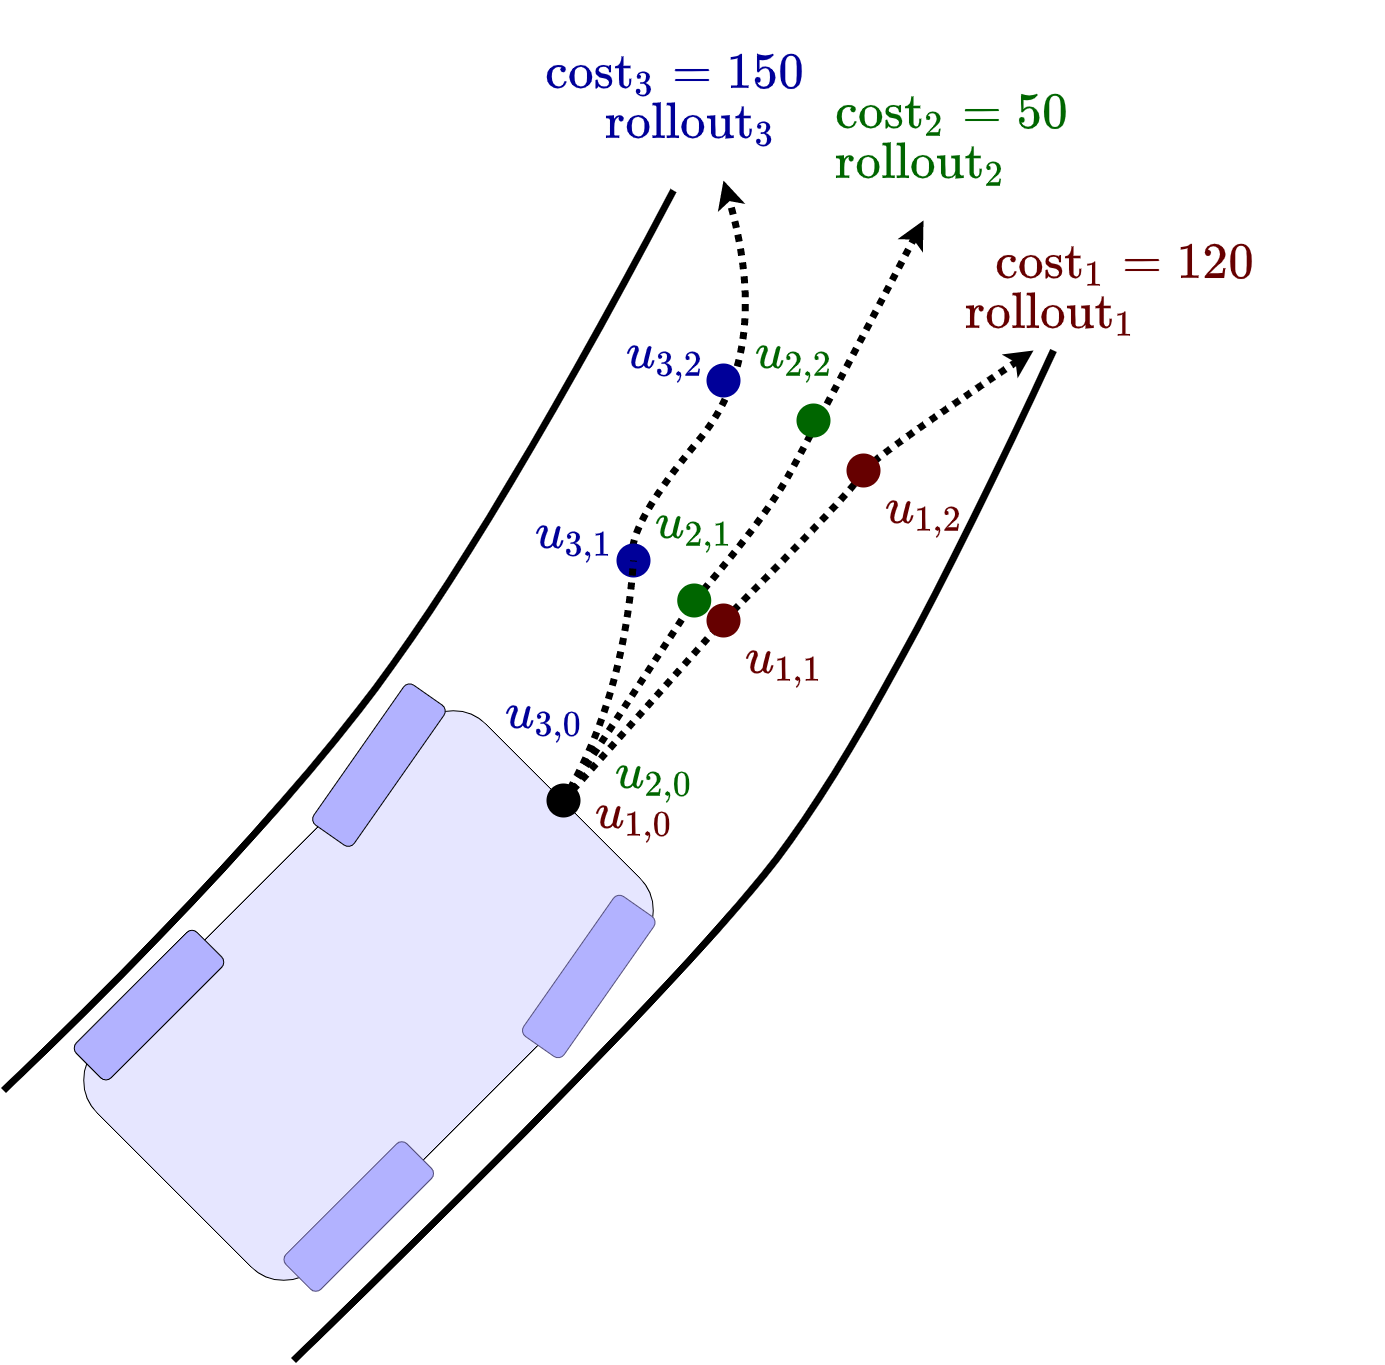
\includegraphics[width=0.5\textwidth]{figures/MPPI_car_with_rollouts.png}
    \caption{\acs{MPPI} controlled race car using a control horizon of 3 time steps, with 3 rollouts all having their respected inputs as $u_{i,j}$ where $i$ is the rollout index and $j$ indicates the time step \cite{neuromorphic_tutorial_ltc21_2021}.}
    \label{figure: mppi_car_with_rollouts}
\end{figure}

Here 3 rollouts are displayed, The objective function is designed to keep the car driving on the center of the road by penalising rollouts which are further away from the center of the road relatively more. resulting in a high cost for $\text{rollout}_1$ and $\text{rollout}_3$ compared to $\text{rollout}_2$. As a result, the input send to the system as a weighted sum of the rollouts is mostly determined by $\text{rollout}_2$. The weighted sum determining the input is displayed in \cref{equation: mppi_weighted_sum}, from \cite{neuromorphic_tutorial_ltc21_2021}.

\begin{equation}
u(k+1)=u(k)+\frac{\sum_{i} w_{i} \delta u_{i}}{\sum_{i} w_{i}}
\label{equation: mppi_weighted_sum}
\end{equation}

Where $\delta u_i$ is the difference between $u(k)$ and the input for rollout $i$, the weight of $\text{rollout}_i$ is detemined as: $w_{i}=e^{-\frac{1}{\lambda} \text{cost}_{i}}$, $\lambda$ is a constant parameter. The reader is now somewhat familiar with the \ac{MPPI} concept, Now some applications with \ac{MPPI} and multi-object control are discussed.\\

From a test pushes train set, \cite{arruda_uncertainty_2017} creates a forward model. The forward model is based on a Gaussian process and can sample multiple trajectories or rollouts in the future, these rollouts are then sent to the \ac{MPPI} controller. While \cite{arruda_uncertainty_2017} was able to create a forward model from scratch, it was unable to improve the forward model after the training phase. This strategy is ideal when the true push dynamics are fully unknown, but makes it less ideal when dynamics change over time.\\

\cite{abraham_model-based_2020} proposed an \ac{EMPPI} controller which requires a partially unknown parameterisable system model of the robot and objects in the environment. Thus this method is as opposed to \cite{arruda_uncertainty_2017} not data-driven. If such a model is provided, \ac{EMPPI} constantly improves the parameterisation found during execution. Which is accomplished by recursively searching for a parameterisation for the partly known dynamics. It is however assumed that the true dynamics reside in the local minima of the parameterisation.\\

Both model identifying methods used in combination with a \ac{MPPI} controller mentioned above need a training set obtained by test pushes. The training phase can only be over when the model results in a stable closed-loop controller. The capability to yield a stable controller is crucial in robotics where time and resources are limited. Currently the fastest stable controller for push manipulation was proposed by \cite{bauza_data-efficient_2018} where the train set required a minimum of only $\sim 10$ train pushes. Then \cite{cong_self-adapting_2020} even claims to require less than 5 train pushes. With the use of a recurrent \ac{LSTM} based model to predict the motion of objects with unknown parameters. The \ac{LSTM}  model provides the \ac{RMPPI} controller with motion predictions. By updating the \ac{LSTM} model and executing \ac{RMPPI} control at the same time the algorithm is self-adapting.\\

\ac{MPPI} has some advantages in comparison to \ac{MPC}. \ac{MPPI} can be optimised by running multiple simulations in parallel. Parallel optimisation improves converging to a control policy \cite{williams_model_2017}. \ac{MPPI} is based on stochastic sampling, this makes the \ac{MPPI} controller naturally take into account nonlinear dynamics, and incorporate nonsmooth/non- differentiable cost functions without approximations \cite{williams_model_2015}, which makes \ac{MPPI} very applicable for multi-body control where the true dynamics mainly are nonlinear. \\ 

\subsection{Intelligent Methods}
\label{subsection: intelligent_methods}
Already seen in previous subsection paper \cite{cong_self-adapting_2020} used a predictive method for control. To identify the system, an intelligent \ac{LSTM} method was used. Intelligent system identification method are seen more often in recent literature, so has \cite{scholz_learning_2015} shown multi-body control using a physics-based reinforcement learning approach. A key advantage intelligent methods provide is the learning speed intelligent methods offer, online adaption is for both \cite{cong_self-adapting_2020} and \cite{scholz_learning_2015} a major advantage over other methods, which makes them very suitable for learning dynamic properties of objects with unknown dynamics. However intelligent methods are out of the scope of this literature because they have trouble generalising. To elaborate, intelligent methods perform very well on the train set, but on unseen data intelligent methods lack performance. The entire point of learning is to be able to generalise to the unseen, even out-of-distribution, and it is currently very difficult to assess learning performance on novel tasks \cite{roy_machine_2021}.\\

Control and identification methods investigated in this literature are conveniently summarised in the following table:

%% TABLE %%%
\begin{table}[H]
\centering
\ra{1.3}
\begin{tabular}{@{}lllllcl@{}}
\rotatebox{30}{\parbox{1.3cm}{System Iden. Type}} & \rotatebox{30}{\parbox{1cm}{Controller Type}} & \rotatebox{30}{\parbox{1.2cm}{Sources}} & \rotatebox{30}{\parbox{1.2cm}{\parbox{1.3cm}{Single-/Multi-body model}}} &  \rotatebox{30}{Requires} &   \rotatebox{30}{ \parbox{1.5cm}{Online Adaptation Model}} &  \rotatebox{30}{\parbox{1.3cm}{Type of model Stored}} \\
\midrule
\multicolumn{4}{l}{\textit{Single-Body Control}} &&&\\
\rowcolor{myEvenLighterColor}  &&&&&&\\[-11pt]
\rowcolor{myEvenLighterColor} &  \shortstack[l]{Fuzzy\\Control\\ \& \ac{PID}}& \cite{ahn_online_2009} & Single  & \shortstack[l]{initial PID\\gains} 
& \cmark & \ac{PID} gains \\
&&&&&&\\[-11pt]
\shortstack[l]{\ac{PEM},\\\ac{IPEM}} & \ac{MPC} & \cite{seegmiller_vehicle_2013}, \cite{farina_convergence_2008} & Single & \shortstack[l]{Nonlinear \\ differential \\ equation}  & \cmark & \shortstack[l]{Calibrated \\nonlinear \\ differential \\ equation} \\
\rowcolor{myEvenLighterColor}  &&&&&&\\[-11pt]
\rowcolor{myEvenLighterColor} - & \shortstack[]{Active\\Inference} & \cite{pezzato_novel_2020}  & Single &   \shortstack[l]{initial\\AI controller\\parameters} & \cmark  & 
\shortstack[l]{belief\\dynamics}\\
\midrule
\multicolumn{2}{l}{\textit{Multi-Body Control}} & & & & &\\
\rowcolor{myEvenLighterColor}  &&&&&&\\[-11pt]
\rowcolor{myEvenLighterColor} - & \shortstack[l]{Reactive\\\ac{MPC}} &\cite{toussaint_sequence--constraints_2022} & \shortstack[l]{Single,\\ Multi} & \shortstack[l]{Dynamical\\model} & \xmark & - \\
 &&&&&&\\[-11pt]
\shortstack[]{Model\\Fitting} & \ac{MPC} &\cite{mericli_push-manipulation_2015}, \cite{bauza_data-efficient_2018} & Multi & \shortstack[l]{sample \\ pushes} & \xmark & \shortstack[]{3D Gaussian\\distribution} \\
\rowcolor{myEvenLighterColor} &&&&&&\\[-11pt]
\rowcolor{myEvenLighterColor}- & unknown &\cite{stuber_feature-based_2018} & Multi & \shortstack[l]{3D object \\point cloud,\\ test pushes}  & \xmark & \shortstack[]{Contact\\model} \\
&&&&&&\\[-11pt]
- & \ac{EMPPI} &\cite{abraham_model-based_2020} & Multi & \shortstack[l]{Partially\\ Unknown\\Dynamics}& \cmark & \shortstack[l]{tuning\\parameters\\Stochastic\\Dynamics}\\
\rowcolor{myEvenLighterColor}  &&&&&&\\[-11pt]
\rowcolor{myEvenLighterColor} \ac{LSTM} & \ac{RMPPI} &\cite{cong_self-adapting_2020} & Multi &   \shortstack[l]{warm up stage,\\contact point} & \cmark & \ac{LSTM}\\
&&&&&&\\[-11pt]
\shortstack[]{Physic-\\based\\Regrssion} & - &\cite{scholz_learning_2015} & Multi & \shortstack[l]{Gripper\\Torques\\for all $t$}& \cmark & \shortstack[l]{Policy}\\
\bottomrule
\end{tabular}
\caption{Summary of interaction approaches and identification methods. The first column displays the model used by the controller, if no model identification method is used this is indicated with a "-". Prior knowledge is indicated in the "Requires" column, poses for single- and multi-bodies are assumed to be known for all time steps. The parameters used to fully store the model are indicated in the last column. }
\label{table: summary_controllers}
\end{table}

\section{Discussion}
\label{section: controllers_discussion}
In \cref{section: system_model_representation} a categorisation of system models is made which are the analytical, data-driven models and hybrid models. Analytical models could be used in situations where a system is fully analysed. Even the robot itself cannot be fully analysed because of slowly changing true dynamics let alone any of the unknown objects. Analytic approaches are for this reason excluded from further investigation. Better suited is the data-driven approach where, with enough data nonlinear parts of the true dynamics are captured, given that enough data is collected and the nonlinear behaviour resides in the data collected. Whilst hybrid models quickly offer a stable model, data-driven models eventually outperform hybrid models. Assuming some structure of the true dynamics allows for obtaining a model fast, while losing from data-driven methods in accuracy during convergence. The hybrid approach is best suited for single-body models, while data-driven methods are best suited for multi-body models. \\

Multiple interaction approaches have been categorised, where predictive methods are the dominant methods. The predictive methods are able to incorporate constraints en uncertainty comparably well. Predictive methods performance heavily depends on the models they use, the system identification method is thus an important factor for stability and overall performance. \\

Many approaches have been discussed to learn dynamical models and their limitations have been emphasised, Because limitations are method-specific the challenge lies in when to choose which interaction approach and which system identification approach. For example, in push manipulation without any prior knowledge the only methods applicable are ones which start with data-driven system identification. Some objects might jump discontinuously between single- and multi-body dynamics (e.g. a ball) such a situation ask for a timing-optimal \ac{MPC}. Objects could be in a corner surrounded by walls, limiting the training phase to only perform test pushes from one side, the best candidate for such a situation would be \ac{LSTM} based controller which requires a minimum amount of training pushes. \\

There is no best interaction approach, different task required different approaches. Mainly the identification approach should be chosen specialised for the task at hand. For robot driving the \ac{MPC} control methods is best suited, using \ac{PEM} for mostly constant system dynamics and \ac{IPEM} for changing system dynamics. Multi-body systems are best controller using \ac{MPPI} control because they naturally incorporate the nonlinear mechanics, the modelling method should take nonlinearities into account, which are data-driven methods such as contact models, or a more complex methods such as \ac{LSTM}. 


\subsection{Motion Planning}%
\label{subsec:motion_planning}

Controllers discussed in \cref{subsec:sys_iden_and_control_methods} can track a path from start to target. Providing a path is a the motion planners responsibility, motion planners seek inside the configuration space for a path from start to target configuration. A practical example of such an path is a list of successive robot poses, from starting pose (coinciding with the starting configuration) toward the target pose, where the successive poses lie close together (reachable for the robot in $\sim20$ time samples). Seeking a path from start to target inside a configuration space whilst avoiding obstacles for the robot to track is referred to as \textit{motion planning}. Finding a path between start and target configuration for pushing application avoiding collision is referred to as \textit{manipulation planning}. First this subsection presents motion planning, next subsection, \cref{subsec:manipulation_planning} dedicates itself to manipulation planning. For both motion and manipulation planning sampling based methods are used, that can be discribed as.\bs

\textit{\quotes{The main idea is to avoid the explicit construction of the object space, and instead conduct a search that probes the configuration space with a sampling scheme. This probing is enabled by a collision detection module, which the motion planning algorithm considers as a “black box.”~\cite{lavalle_planning_2006}}}\bs

Generally the configuration space motion planners plan in consists of 2 subspaces, free and obstacle space. The configuration space in this thesis consists of 4 subspaces, namely free, obstacle, unknown and movable space. To solve motion planning problems for such a configuration space a dedicated motion planning algorithm has been developed that extends the existing algorithm extends the existing double tree \ac{RRT*} algorithm~\cite{chen_fast_2018}. The motion planner consists of.
\begin{center}
\begin{tabular}[t]{l p{10cm}}
$V$:& A set of nodes\\
$E$:& A set of edges\\
$P$:& A set of paths\\
\end{tabular}
\end{center}

The start connectivity tree consists of the nodes connected by edges containing the starting node, and vise versa for the target connectivity tree containing the target node. The algorithm grows the two \textit{connectivity trees} by randomly sampling configurations and adding them to the start or target connectivity tree. The algorithm explores configuration space by growing these connectivity trees. When the start connectivity tree meets the target connectivity tree a path from start to target is found.\bs

Newly sampled configurations are added is a structural manner that guarantee an optimal path is found with infinite sampling. Where optimality is defined as the path with the lowest cost. The cost is defined as a sum of a distance metric and a fixed penalty for paths that cross unknown or movable subspaces. Incentivising the algorithm to find a path around unknown or movable obstacles over path crossing through unknown or movable obstacles.\bs

The algorithm takes in 2 arguements, first the \textit{step size}, an maximal normalised distance between connected samples in the connectivity trees. Second, the \textit{search size} an subspace around newly sampled samples, inside this subspace a parent node is saught that results in the lowest cost, rewiring of closeby nodes happens and the other connectivity tree is searched to detects a full path form start to target.\bs

Now pseudocode of the proposed algorithm is provided in \cref{pseudocode:proposed_rrt_star}, functions used are elaborated on in \cref{table:functions_for_proposed_rrt_star}. The colored sections inside \cref{pseudocode:proposed_rrt_star} correspond the the surrounding colored box around subfigures in \cref{fig:motion_planner_adding_one_sample}. The following definitions are used by the proposed algorithm.\bs

\begin{table}[H]
\centering
\begin{tabular}[t]{l p{10cm}}
$x$:& A node containing a point in configuration space\\
$x_{init}$:& Creates a start and target node\\ 
$NotReachStop$:& True if the stopping criteria is not reached\\ 
$Sample_{random}$:& Creates a random sample in free-, movable- or unknown space\\
$Nearest(x, V)$:& Returns the nearest nodes from $x$ in $V$\\
$NearestSet(x, V)$:& Returns set of nearest nodes from $x$ in $V$\\
$Project(x, x')$:& Project $x$ toward $x'$\\
$CollisionCheck(x)$:& Returns true if $x$ is in free-, movable- or unknown space\\
$ObjectCost(x', x)$:& Returns a fixed additional cost if $x$ enters movable- or unknown space from $x'$, otherwis returns 0\\
$Distance(x, x')$:& Returns the distance between sample $x$ and $x'$\\
$CostToInit(x)$:& Find the total cost from $x$ to the initial node\\
$LocalPlannerCheck(x, x')$:& Return true if a local planner is able to connect $x$ and $x'$, otherwise return false. A system model (see \cref{subsec:sys_iden_and_control_methods}) acts a local planner\\
$InSameTree(x, x')$:& Returns true if both $x$ and $x'$ are in the same tree, otherwise return false\\
\end{tabular}
\caption{Functions used by the \cref{pseudocode:proposed_rrt_star}}
\label{table:functions_for_proposed_rrt_star}
\end{table}

\newpage
\begin{algorithm}[H]
\caption{Pseudocode for modified $\text{RRT}^*$ algorithm taking movable objects and constraints into account}
\label{pseudocode:proposed_rrt_star}
\begin{algorithmic}[1]

\hspace{-0.9cm}\colorbox{my_grey}{\parbox{\linewidth}{%
\State $V \leftarrow x_{init}$
\While{$NotReachStop$} 

\hspace{-0.1cm}\colorbox{my_light_blue}{\parbox{\linewidth}{%
    \State $Cost_{min} \leftarrow +\infty$ \algorithmiccomment{Create, check and project a new random sample}
    \State $x_{rand} \leftarrow Sample_{random}$
    \State $x_{nearest} \leftarrow Nearest(x_{rand}, V)$
    \State $x_{temp} \leftarrow Project(x_{rand}, x_{nearest})$

    \If{$CollisionCheck(x_{temp})$}
        \State $x_{new} = x_{temp}$
        \Else
        \State $Continue$
    \EndIf
}}

\hspace{-0.1cm}\colorbox{my_yellow}{\parbox{\linewidth}{%
    \State $X_{near} \leftarrow NearestSet(x_{new}, V)$ \algorithmiccomment{Find and connect new node to parent node}
    \For{$x_{near} \in X_{near}$}
    \State $Cost_{temp} \leftarrow CostFromInit(x_{near}) + Distance(x_{near}, x_{new}) + ObjectCost(x_{near}, x_{new})$
    \If{$Cost_{temp}  < Cost_{min}$}
            \If{$LocalPlannerCheck(x_{new}, x_{near})$}
            \State $Cost_{min} \leftarrow x_{temp}$
            \State $x_{minCost} \leftarrow x_{near}$
            \EndIf
        \EndIf
    \EndFor
    \If{$Cost_{min} == \infty$}
        \State $Continue$
    \Else
        \State $V.add(x_{new})$
        \State $E.add(x_{minCost}, x_{new})$
    \EndIf
}}

\hspace{-0.1cm}\colorbox{my_green}{\parbox{\linewidth}{%
    \State $Cost_{path} \leftarrow +\infty$ \algorithmiccomment{Check if newly added node can lower cost for nearby nodes}
    \For{$x_{near} \in X_{near}$} 
      \If{$InSameTree(x_{near}, x_{new})$} 
        \State $Cost_{temp} \leftarrow CostFromInit(x_{new}) + distance(x_{new}, x_{near}) + ObjectCost(x_{new}, x_{near})$
        \If{$Cost_{temp} < CostFromInit(x_{near})$}
           \If{$LocalPlannerCheck(x_{new}, x_{near})$}
              \State $E.rewire(x_{near}, x_{new})$
           \EndIf
        \EndIf
      \Else \algorithmiccomment{Add lowest cost path to list of paths}
          \State $Cost_{temp} \leftarrow CostFromInit(x_{new}) + distance(x_{new}, x_{near}) $ \newline\hspace*{10em} $+ CostFromInit(x_{near}) + ObjectCost(x_{new}, x_{near})$
          \If{$Cost_{temp}  < Cost_{path}$}
              \If{$LocalPlannerCheck(x_{new}, x_{near})$}
                  \State $Cost_{pathMin} \leftarrow x_{temp}$
                  \State $x_{pathMin} \leftarrow x_{near}$
              \EndIf
          \EndIf
      \EndIf
      \If{$Cost_{pathMin} == \infty$}
          \State $Continue$
      \Else
          \State $P.addPath(x_{new}, x_{pathMin}, Cost_{pathMin})$
      \EndIf
    \EndFor
}}

\EndWhile
}}
\end{algorithmic}
\end{algorithm}

\newpage
Now an example is provided of the proposed algorithm that creates and adds one sample in \cref{fig:motion_planner_adding_one_sample}. After adding the newly sampled sample is added tot the start connectivity tree, a sample is rewired then the target connectivity tree is connected to the start connectivity tree. The resulting path found can be visualised in \cref{fig:motion_planner_comparison}.\bs

\begin{figure}[H]
    \centering
    \begin{subfigure}{.49\textwidth}
    \centering
    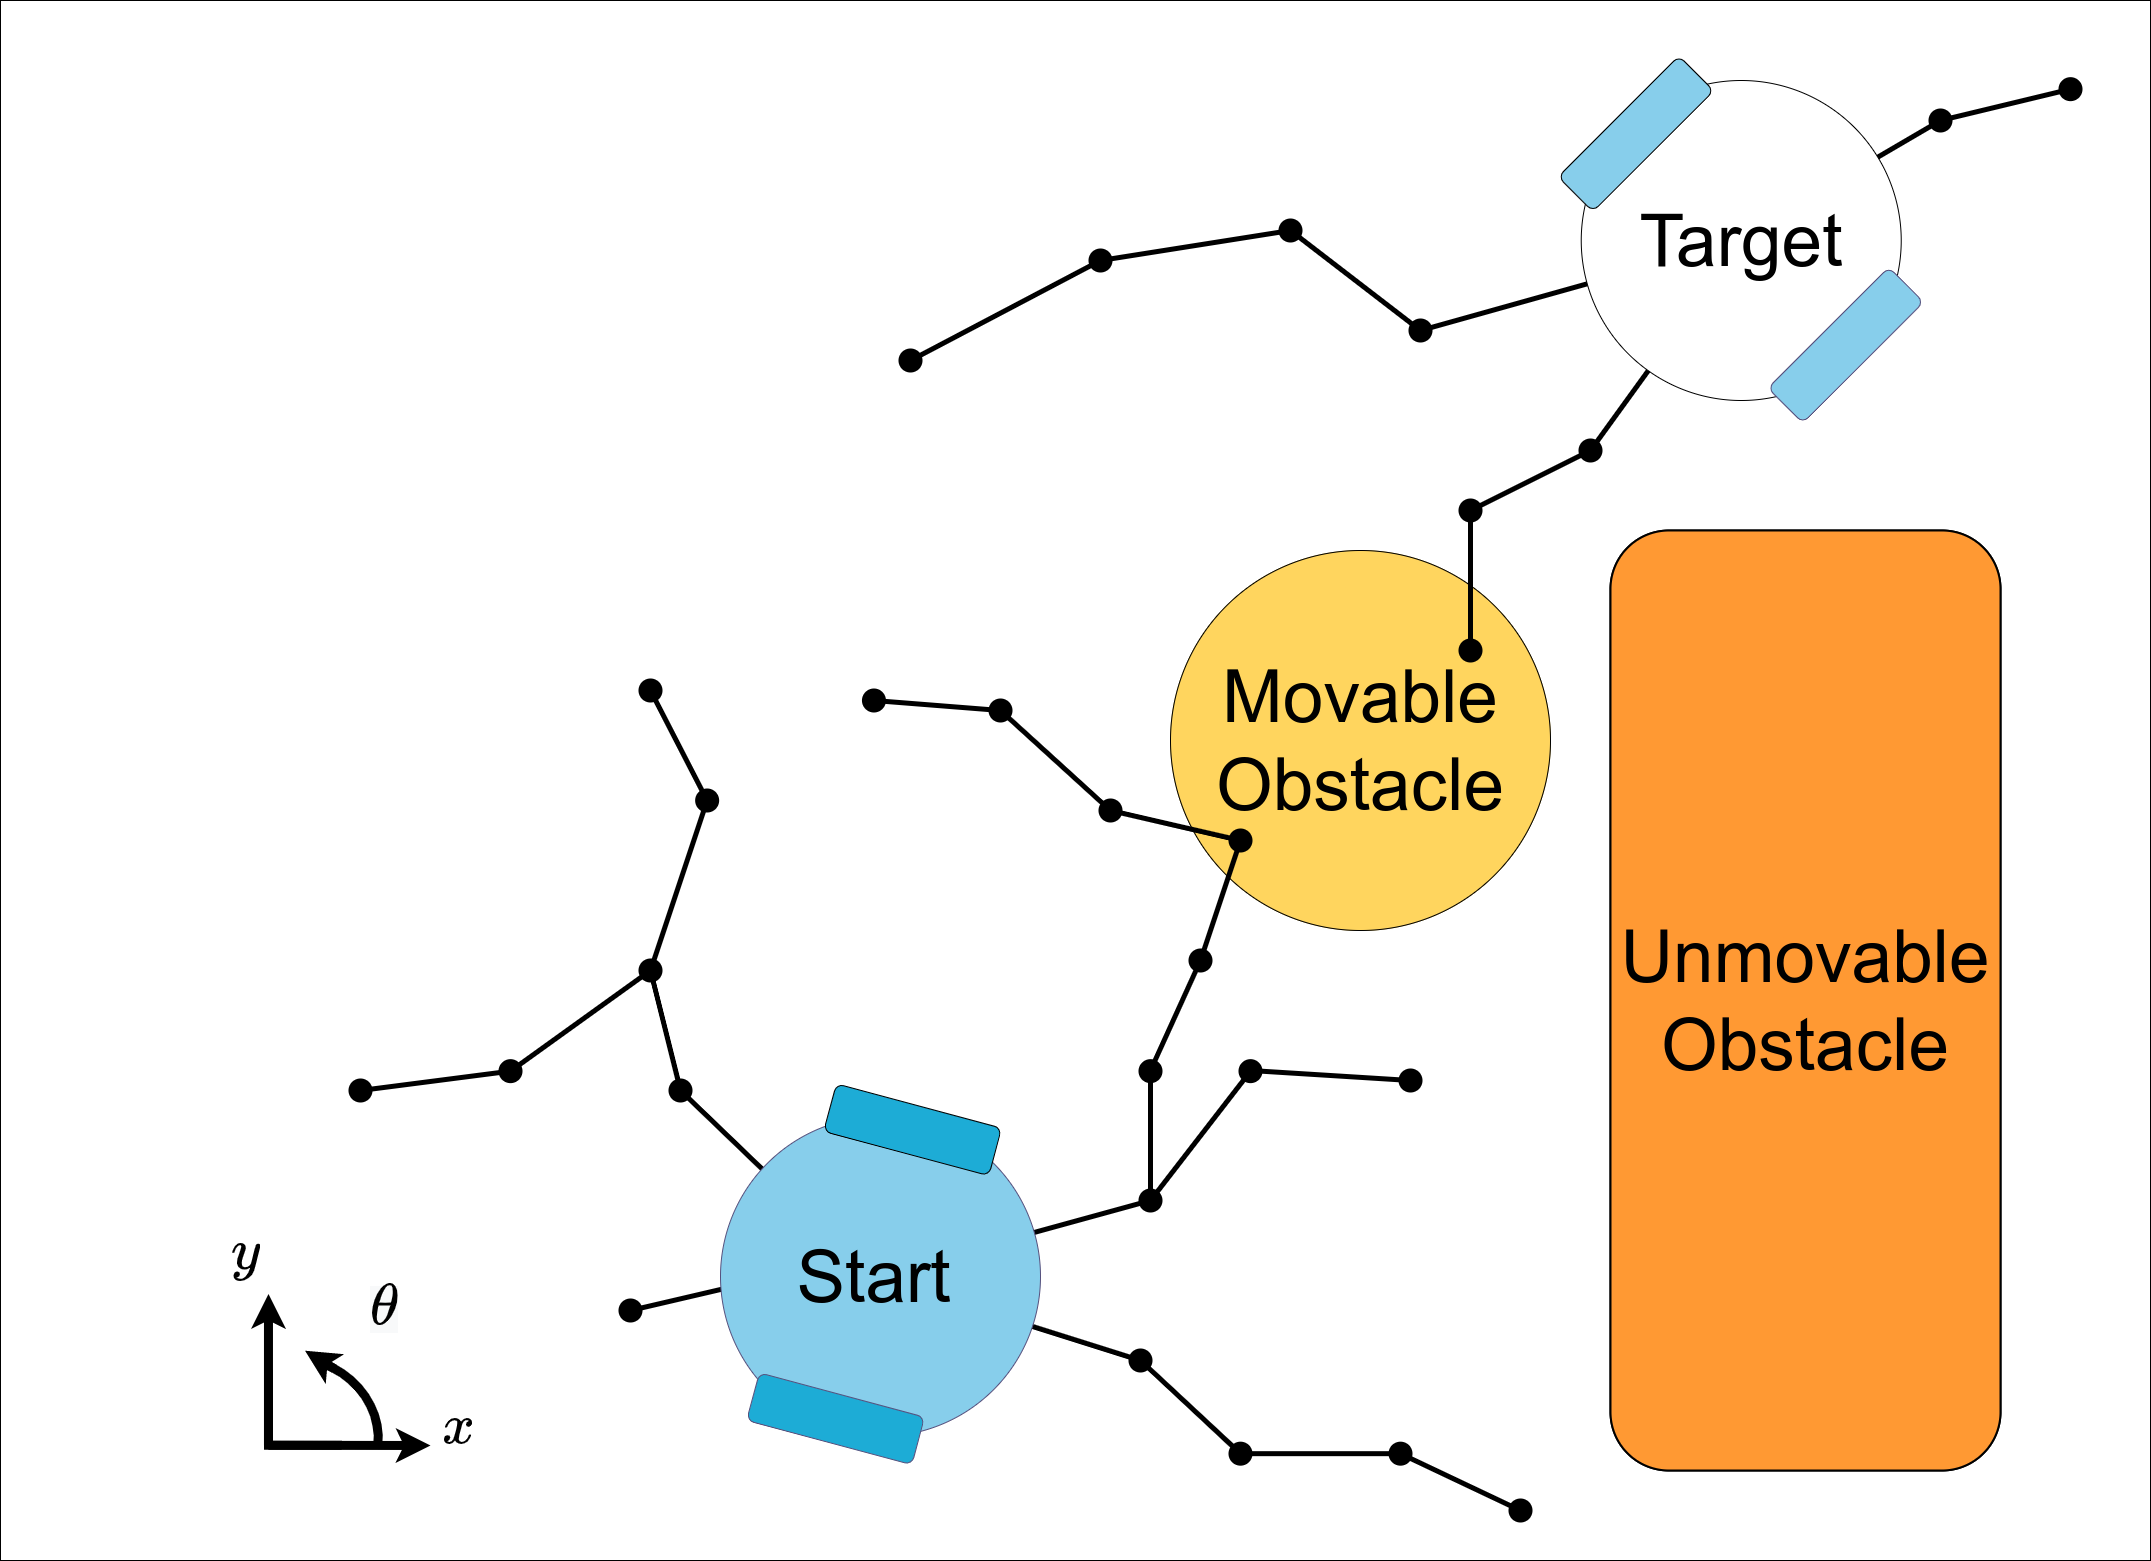
\includegraphics[width=0.93\textwidth, cfbox=my_grey 5pt 0pt]{figures/mp/1mp_init.drawio.png}
    \caption{Snapshot of the configuration space during a search\\from start to target configuration.}
    \end{subfigure}
    \begin{subfigure}{.49\textwidth}
    \centering
    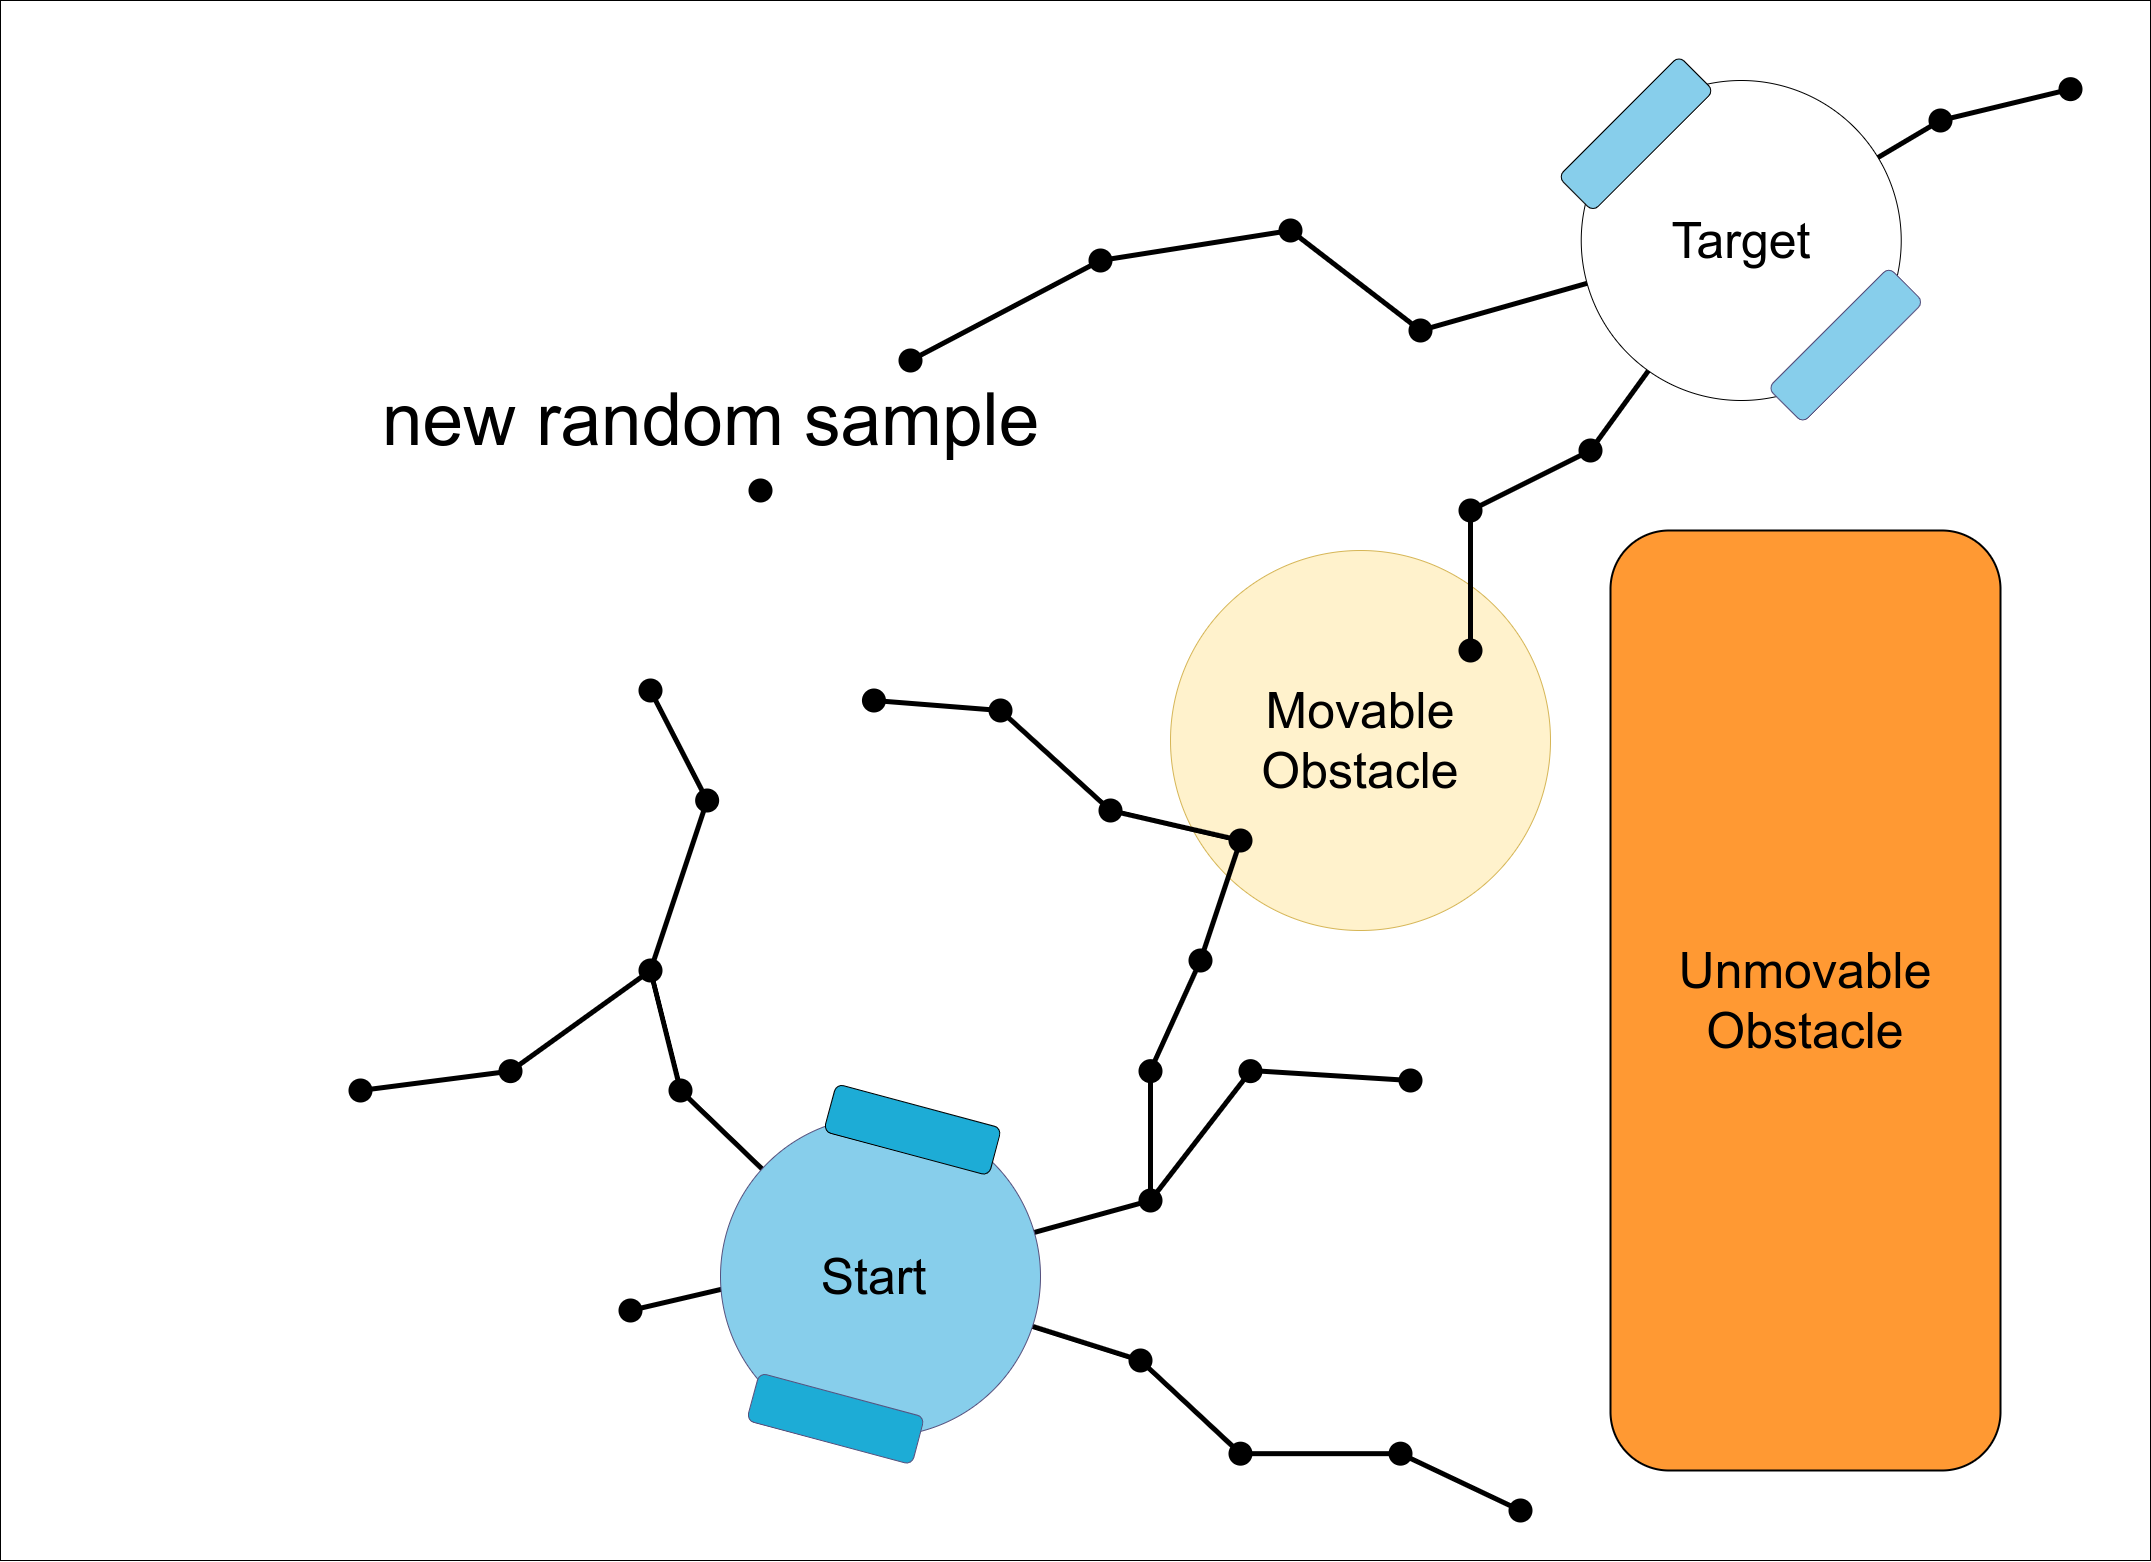
\includegraphics[width=0.93\textwidth, cfbox=my_light_blue 5pt 0pt]{figures/mp/2mp_new_rand_sample.drawio.png}
    \caption{A new random sample is generated.\bs}
    \end{subfigure}

    \begin{subfigure}{.49\textwidth}
    \centering
    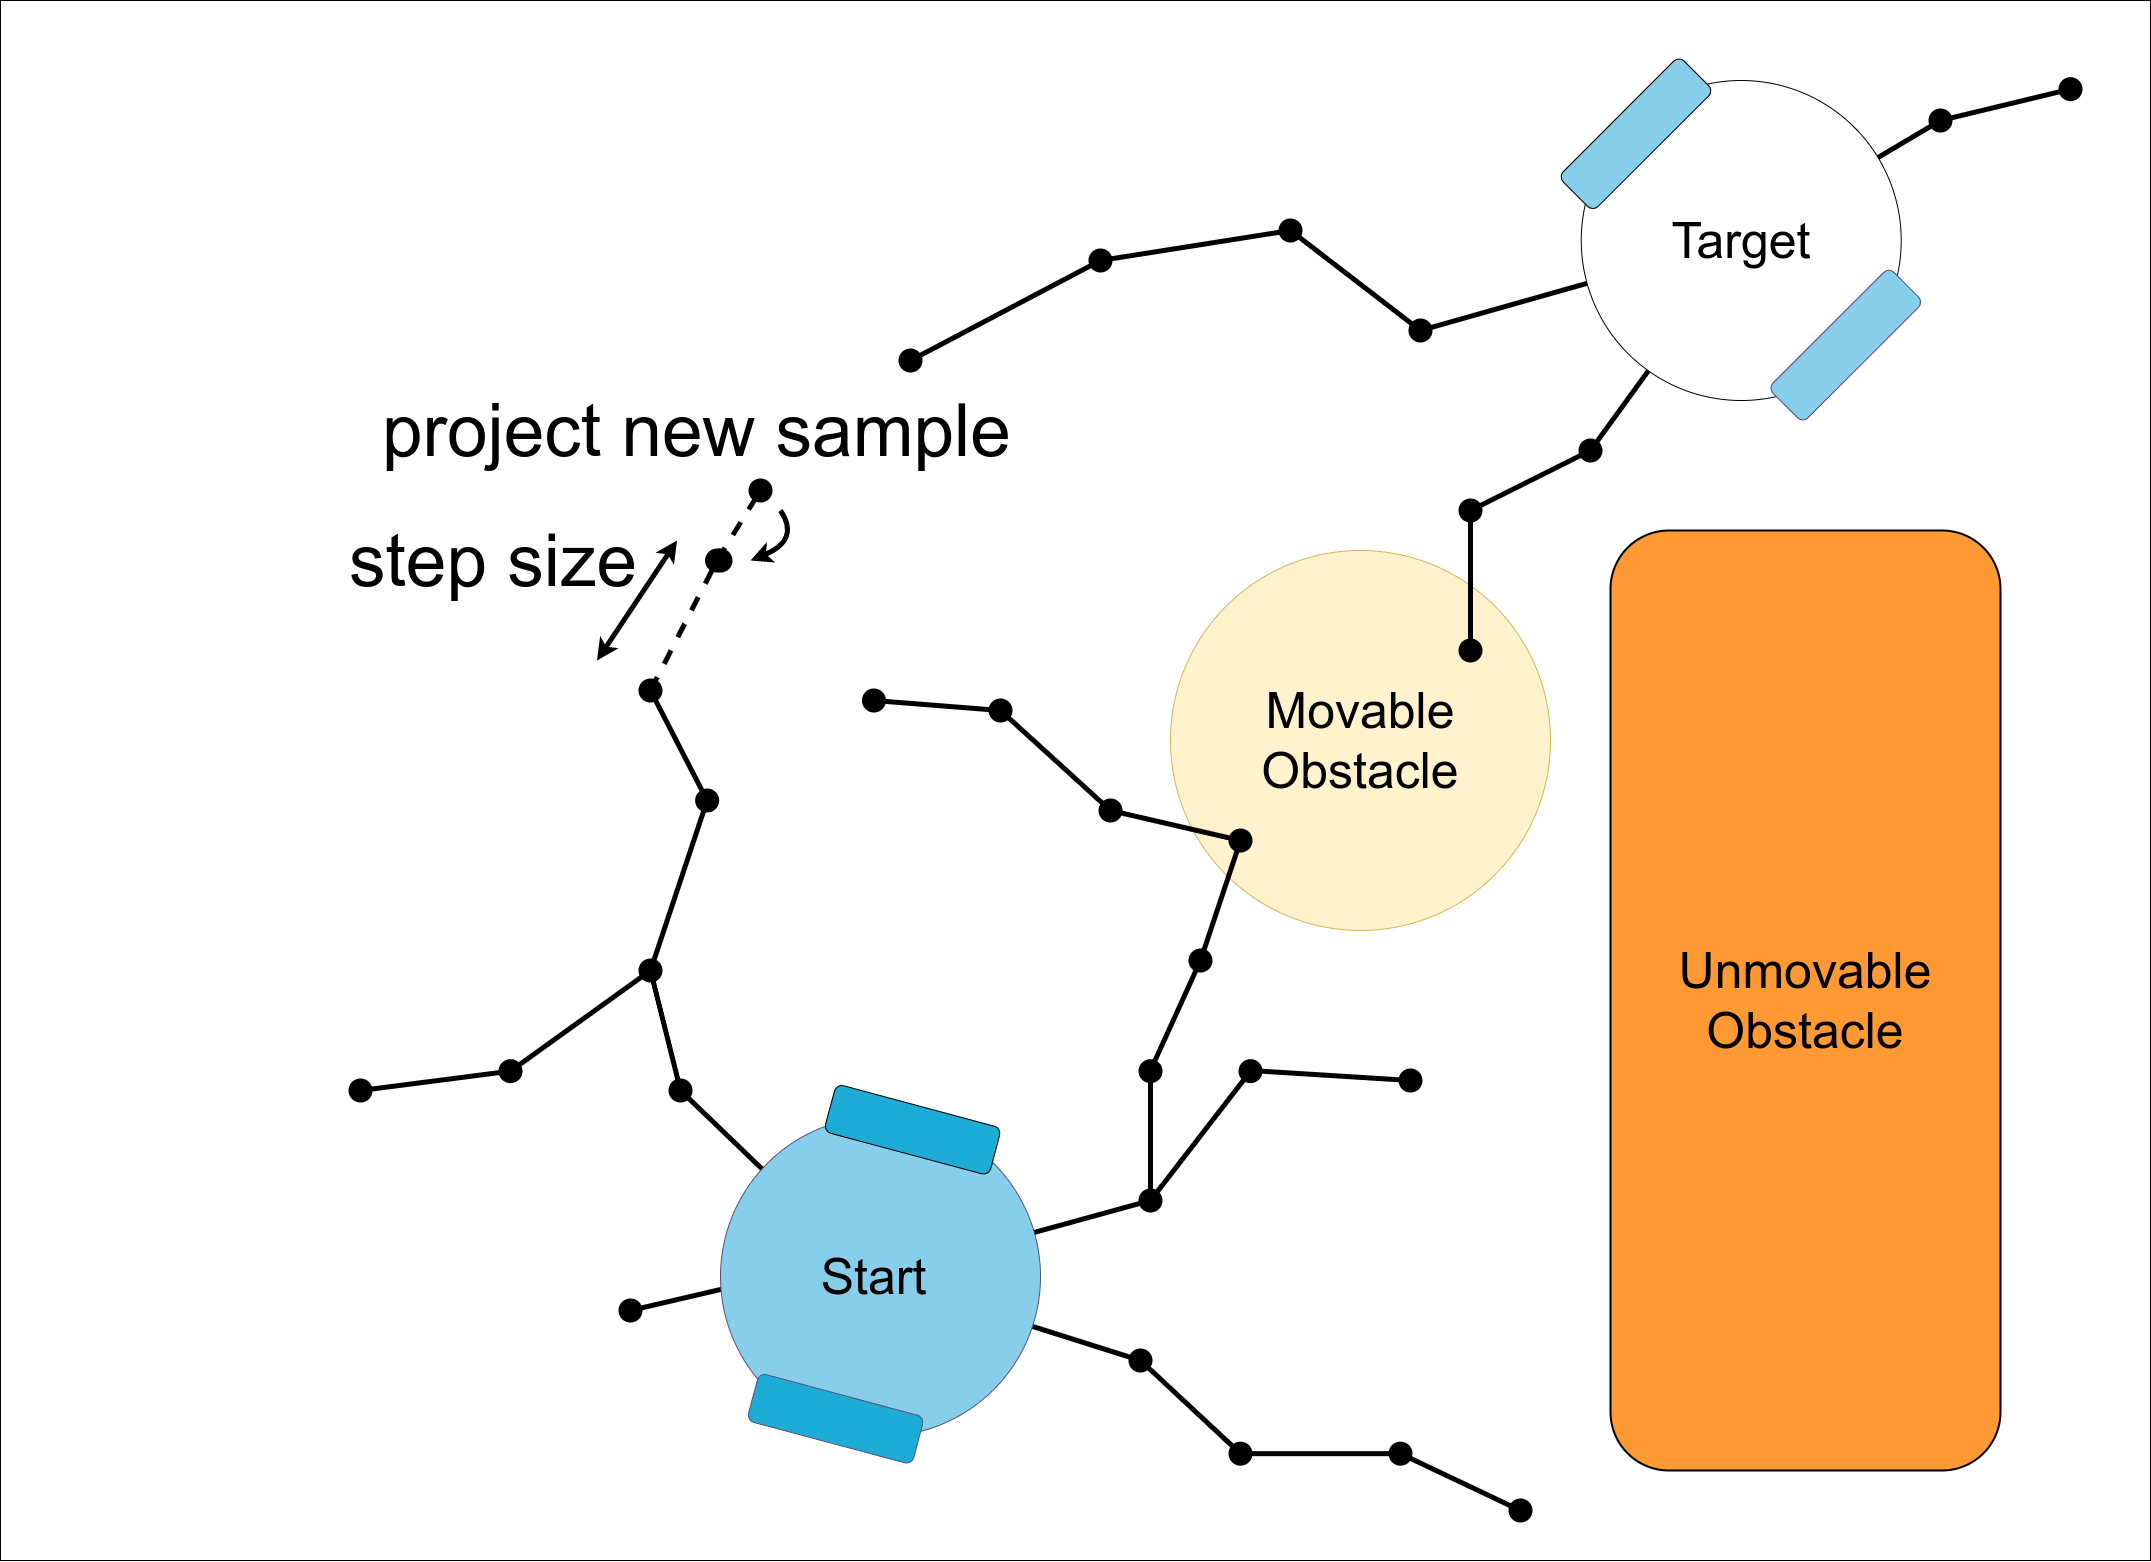
\includegraphics[width=0.93\textwidth, cfbox=my_light_blue 5pt 0pt]{figures/mp/3mp_project_sample.drawio.png}
    \caption{The new sample is projected toward the closest sample.\bs}
    \end{subfigure}
    \begin{subfigure}{.49\textwidth}
    \centering
    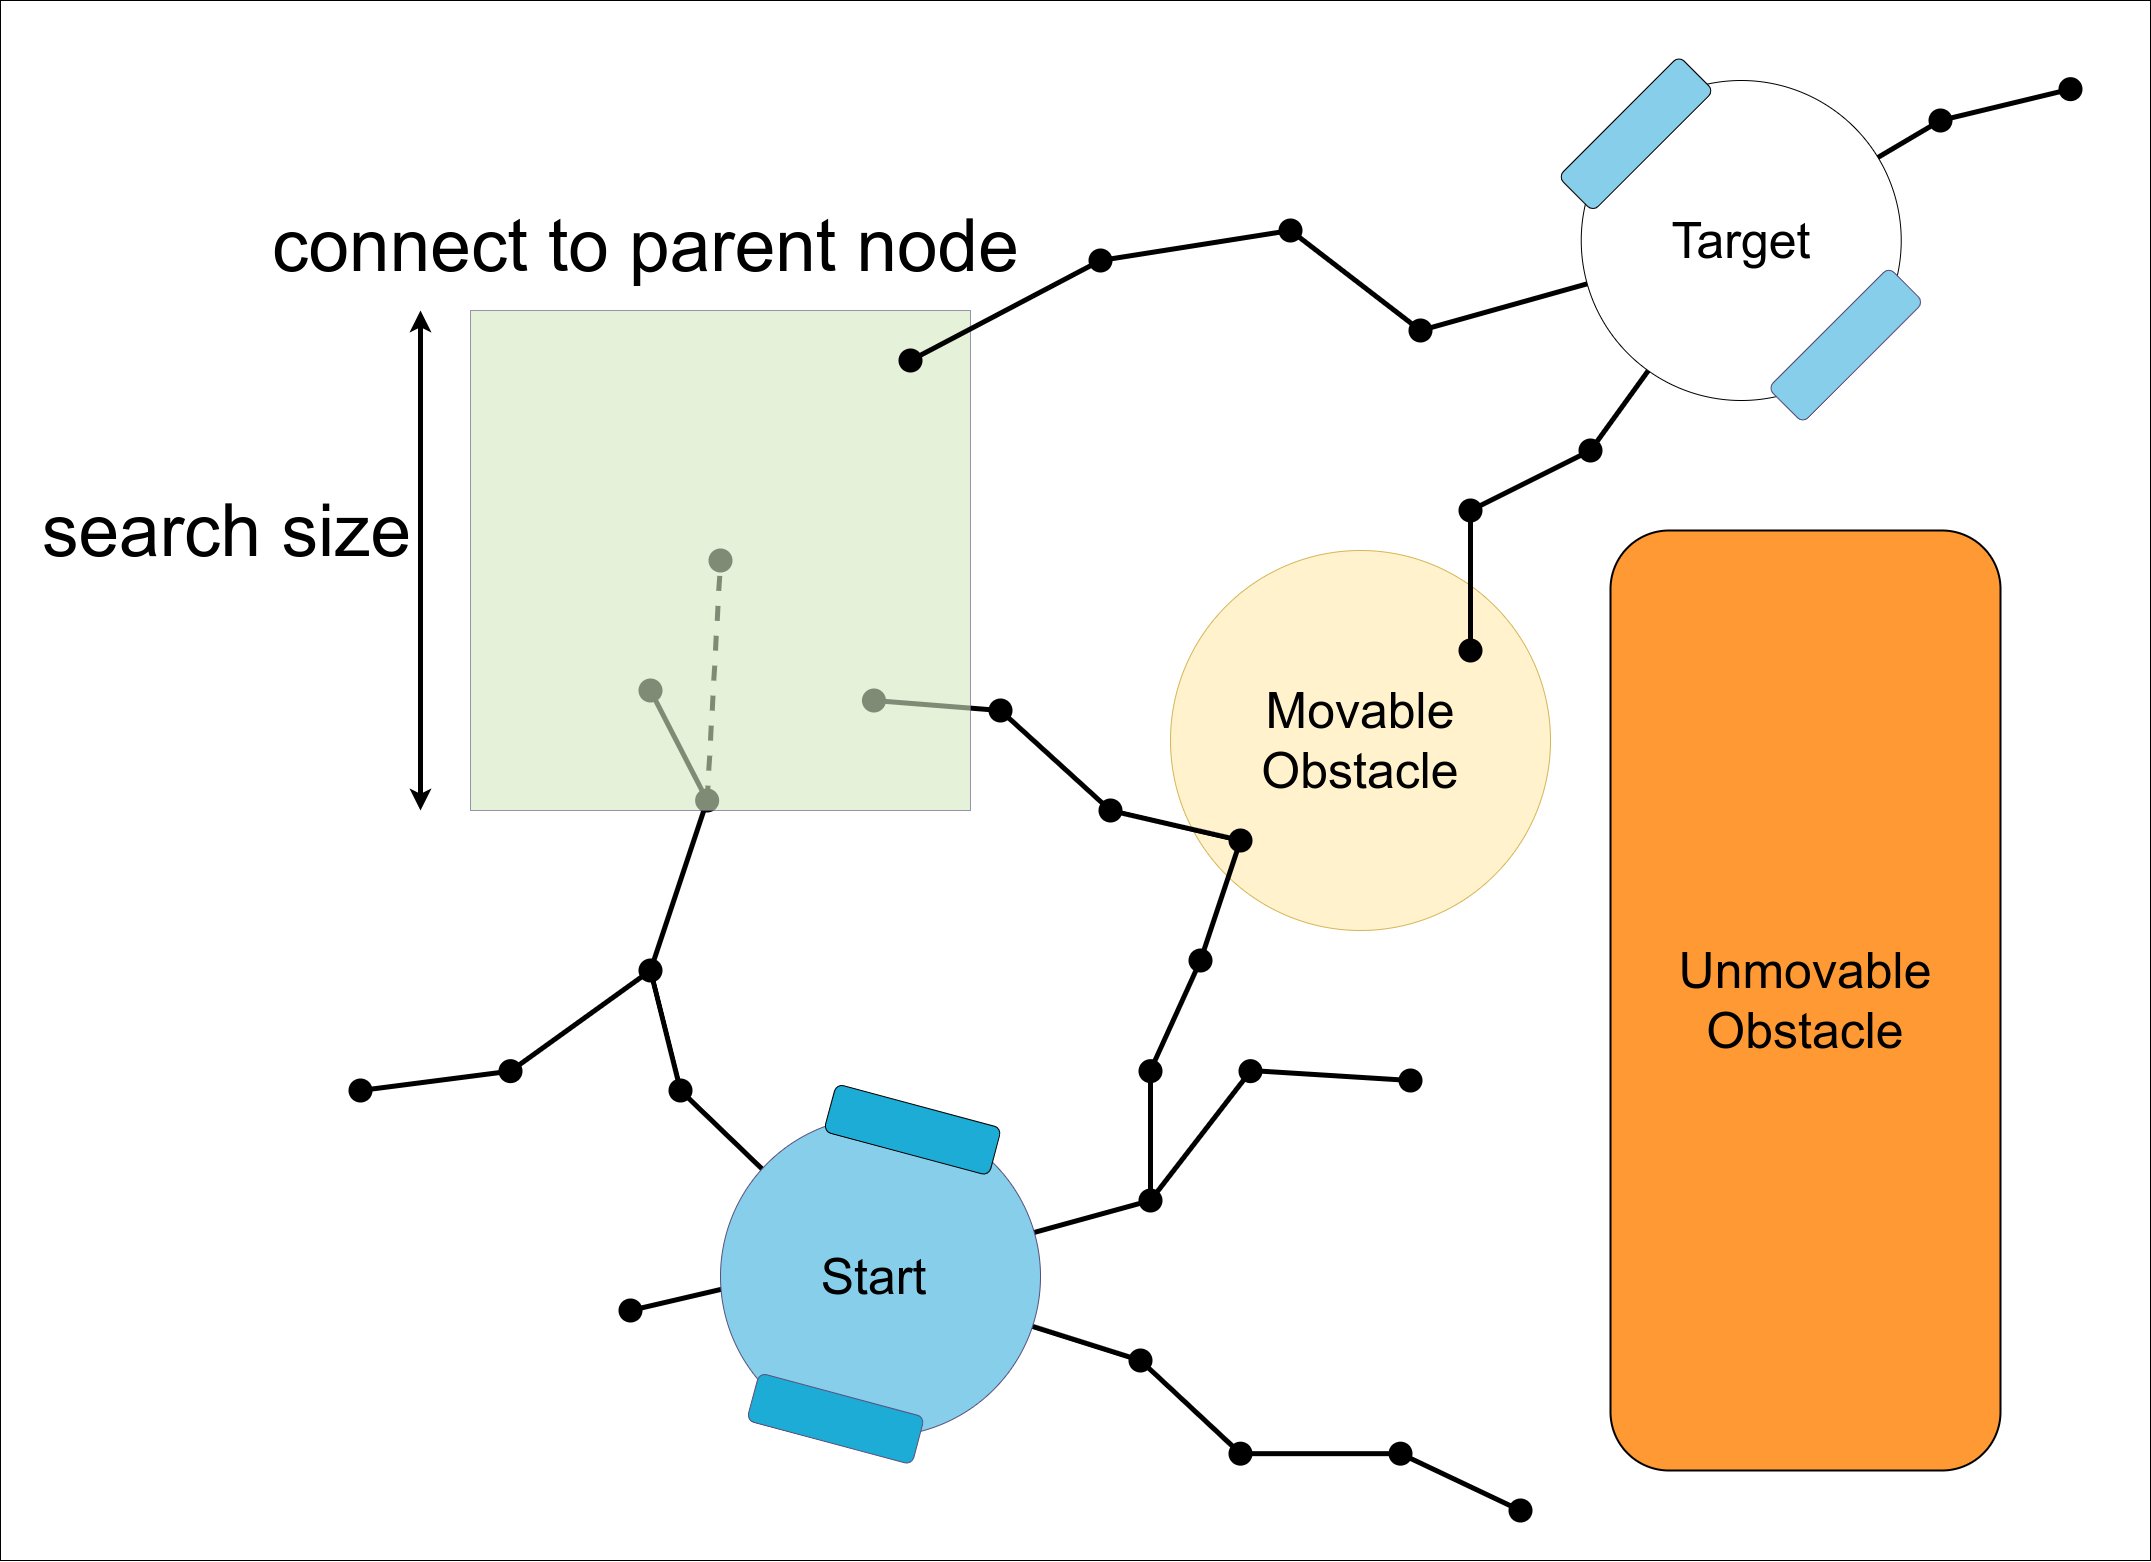
\includegraphics[width=0.93\textwidth, cfbox=my_yellow 5pt 0pt]{figures/mp/4mp_connect_to_tree.drawio.png}
    \caption{The new sample is connected to the node in search space\\that results in the lowest cost.}
    \end{subfigure}

    \begin{subfigure}{.49\textwidth}
    \centering
    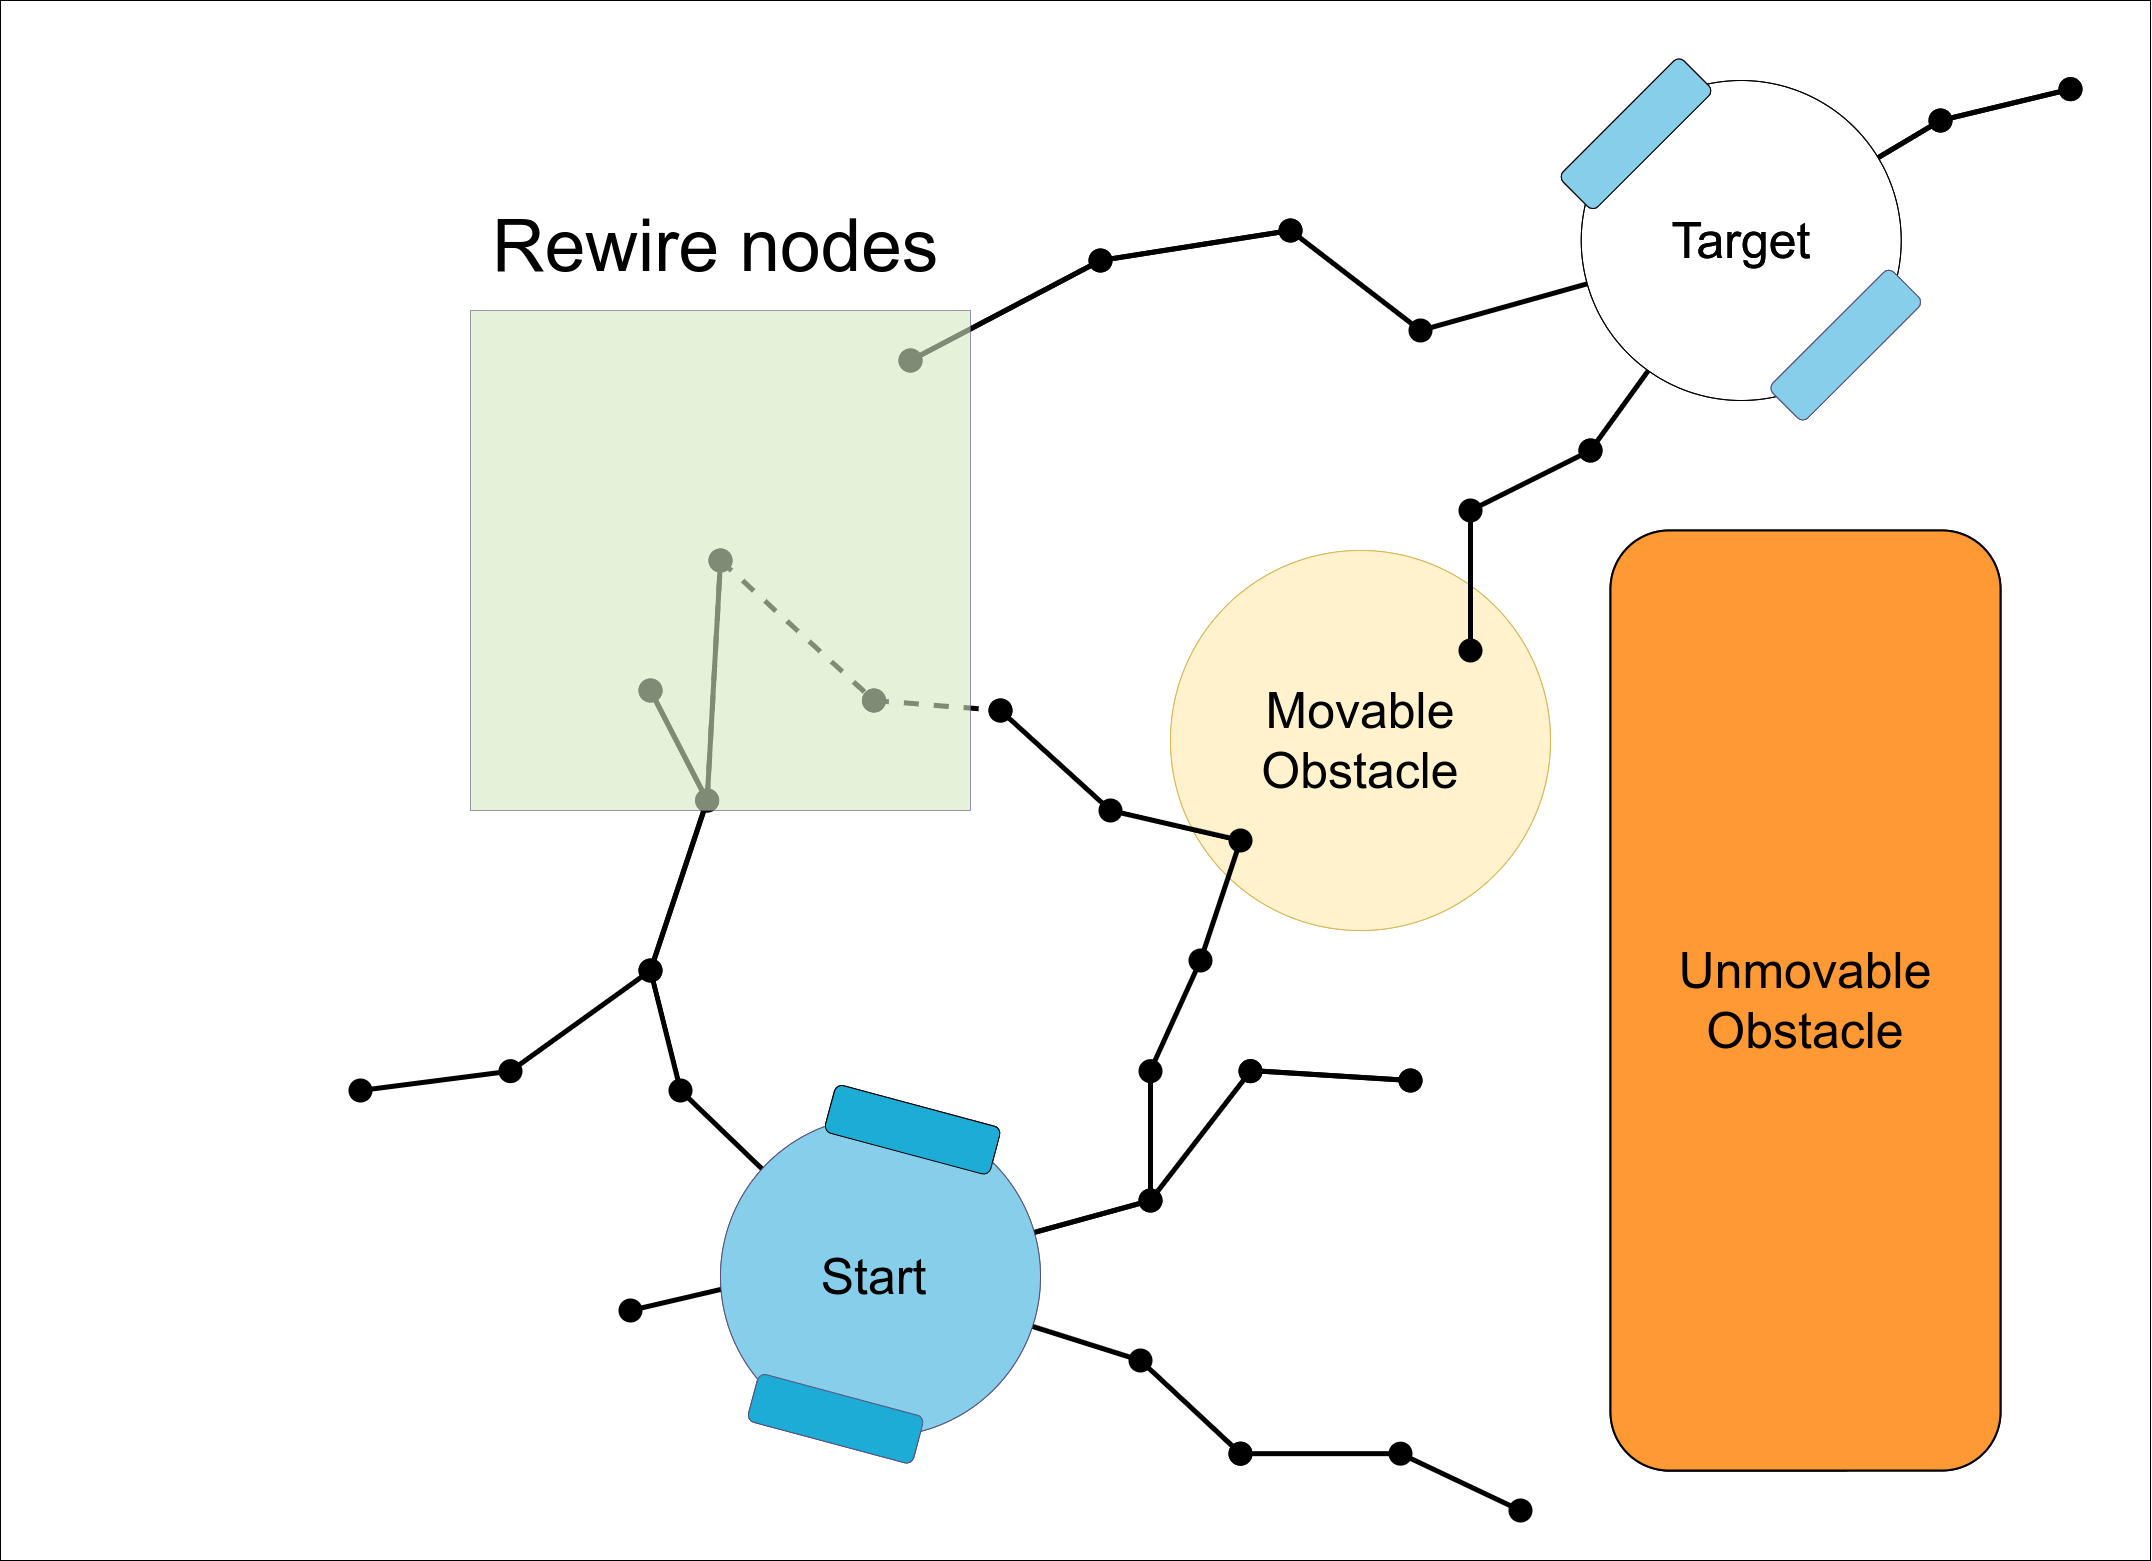
\includegraphics[width=0.93\textwidth, cfbox=my_green 5pt 0pt]{figures/mp/5mp_rewire.drawio.png}
    \caption{Nodes for which the cost can be lowered\\from the new sample are rewired.}
    \end{subfigure}
    \begin{subfigure}{.49\textwidth}
    \centering
    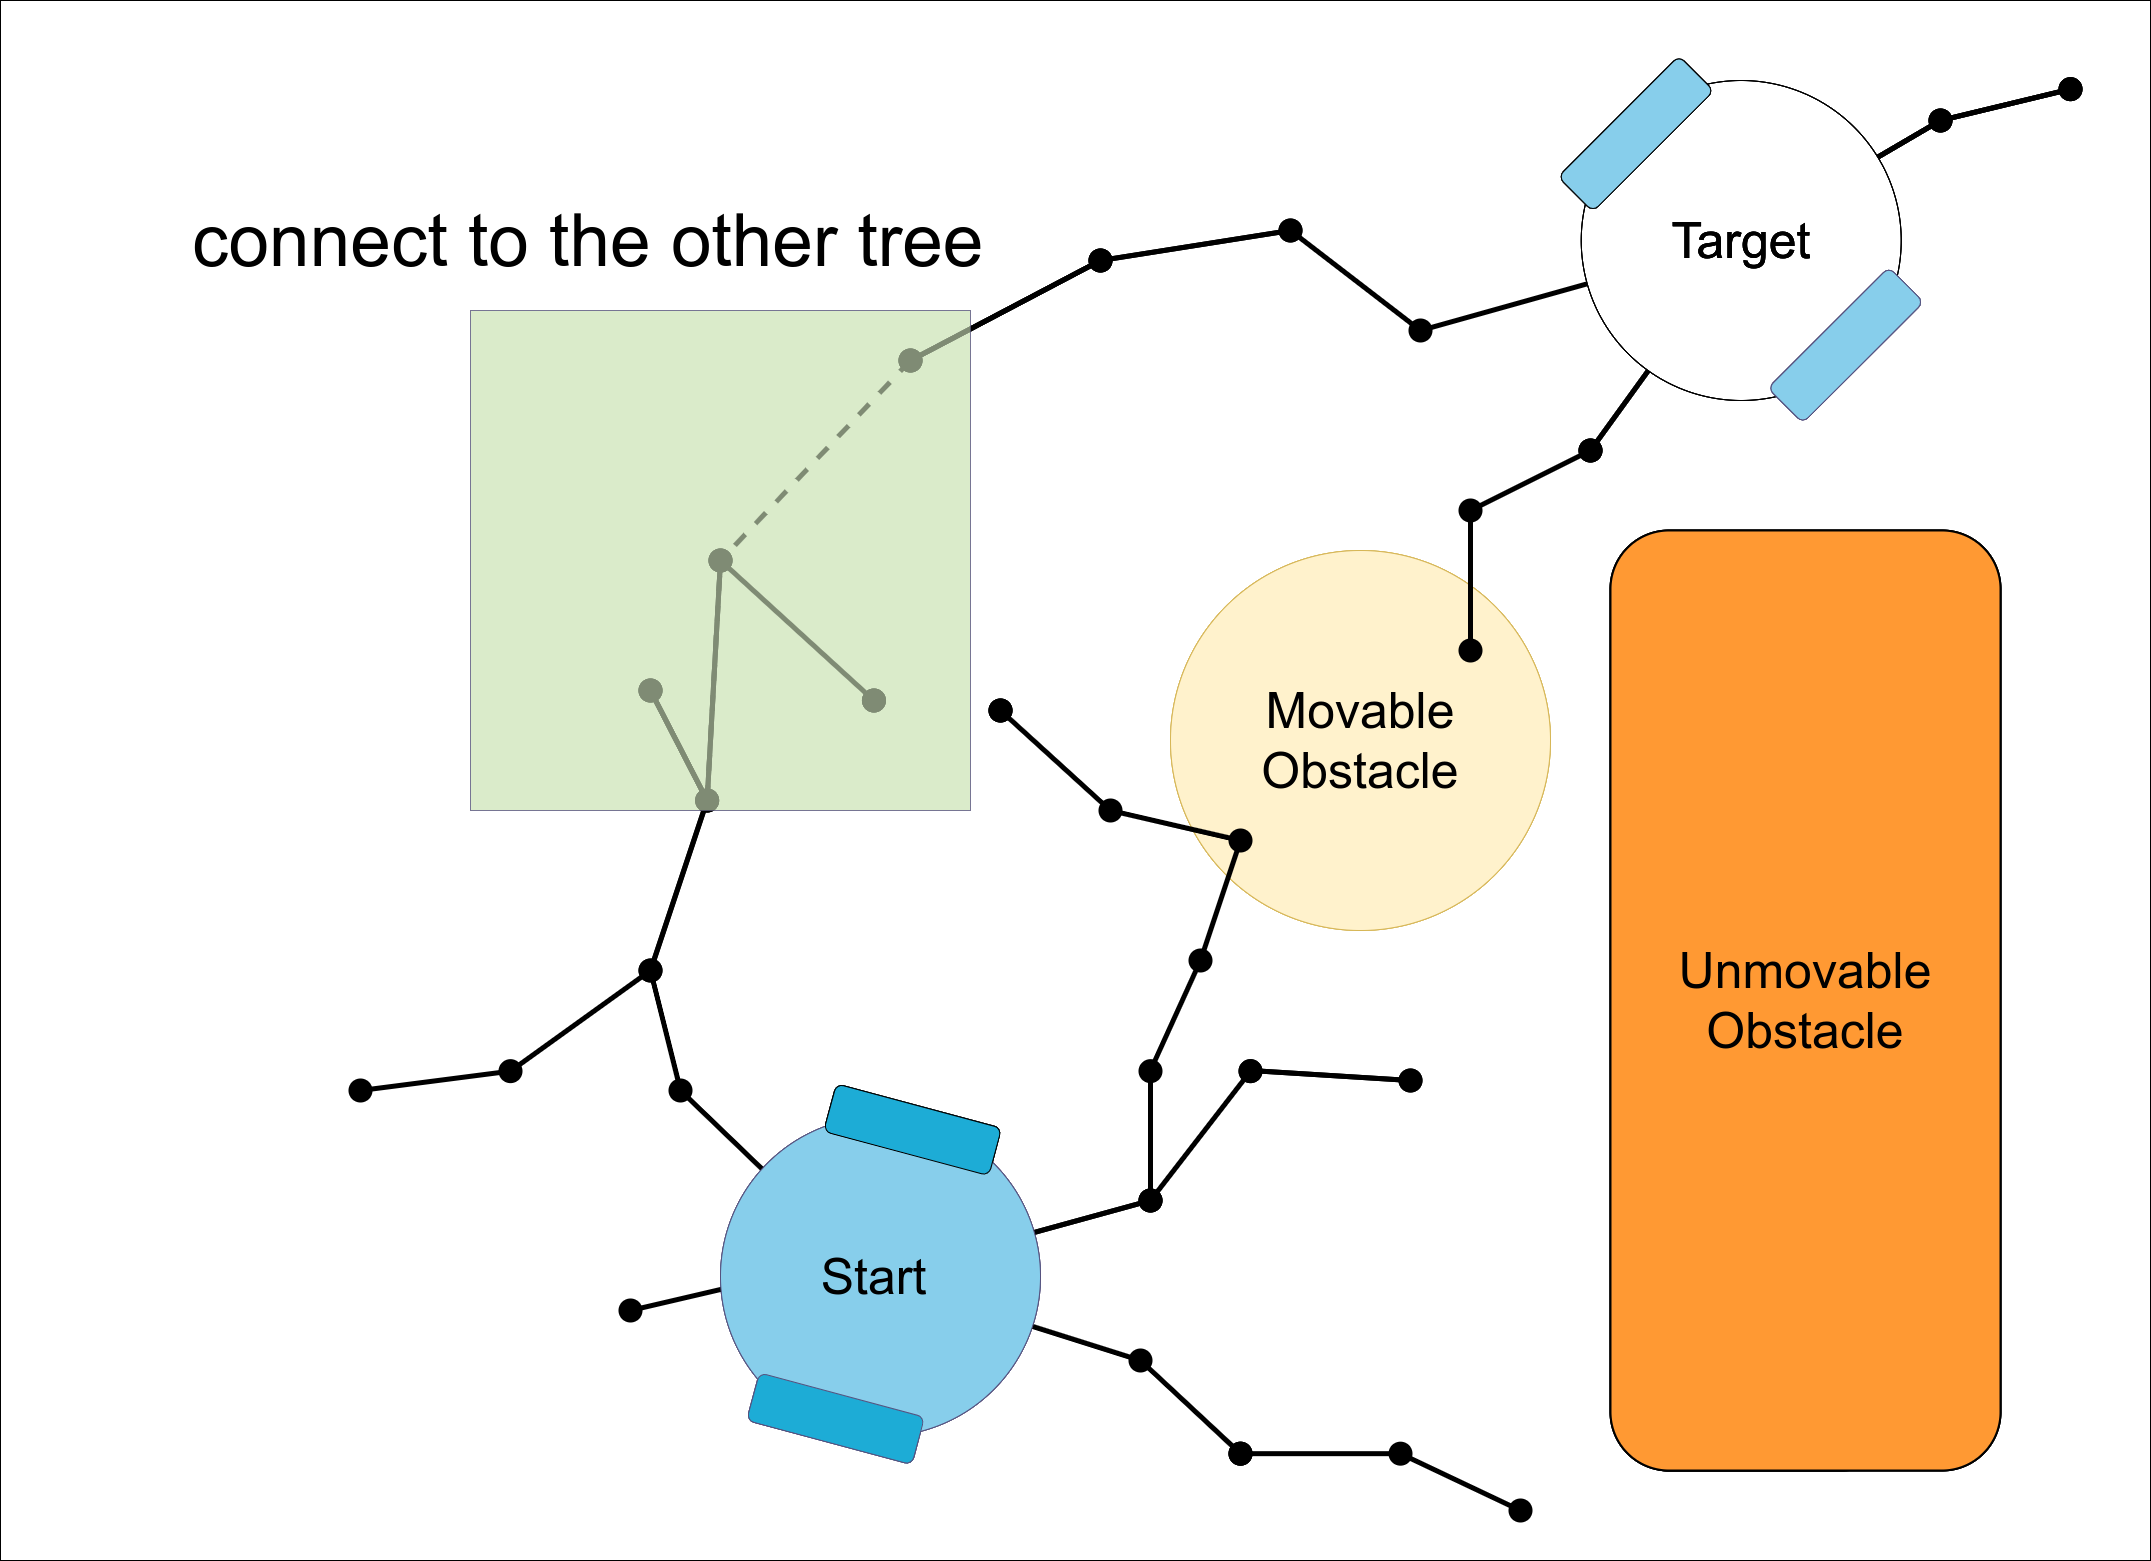
\includegraphics[width=0.93\textwidth, cfbox=my_green 5pt 0pt]{figures/mp/6mp_search_other_tree.drawio.png}
    \caption{A path from start to target configuration is found. \bs}
    \end{subfigure}

    \caption{Visualisation of the Double tree \acs{RRT*} motion planner that add a single sample to the connectivity graph. The color of the box surrounding subfigures corresponds to the colored sections in \cref{pseudocode:proposed_rrt_star}. 3 dimensional configuration space displayed as 2 dimensional configuration space ($x$ and $y$ are visable, $\theta$ is not visable).}
    \label{fig:motion_planner_adding_one_sample}
\end{figure}


\begin{figure}[H]
    \centering
    \begin{subfigure}{.5\textwidth}
    \centering
    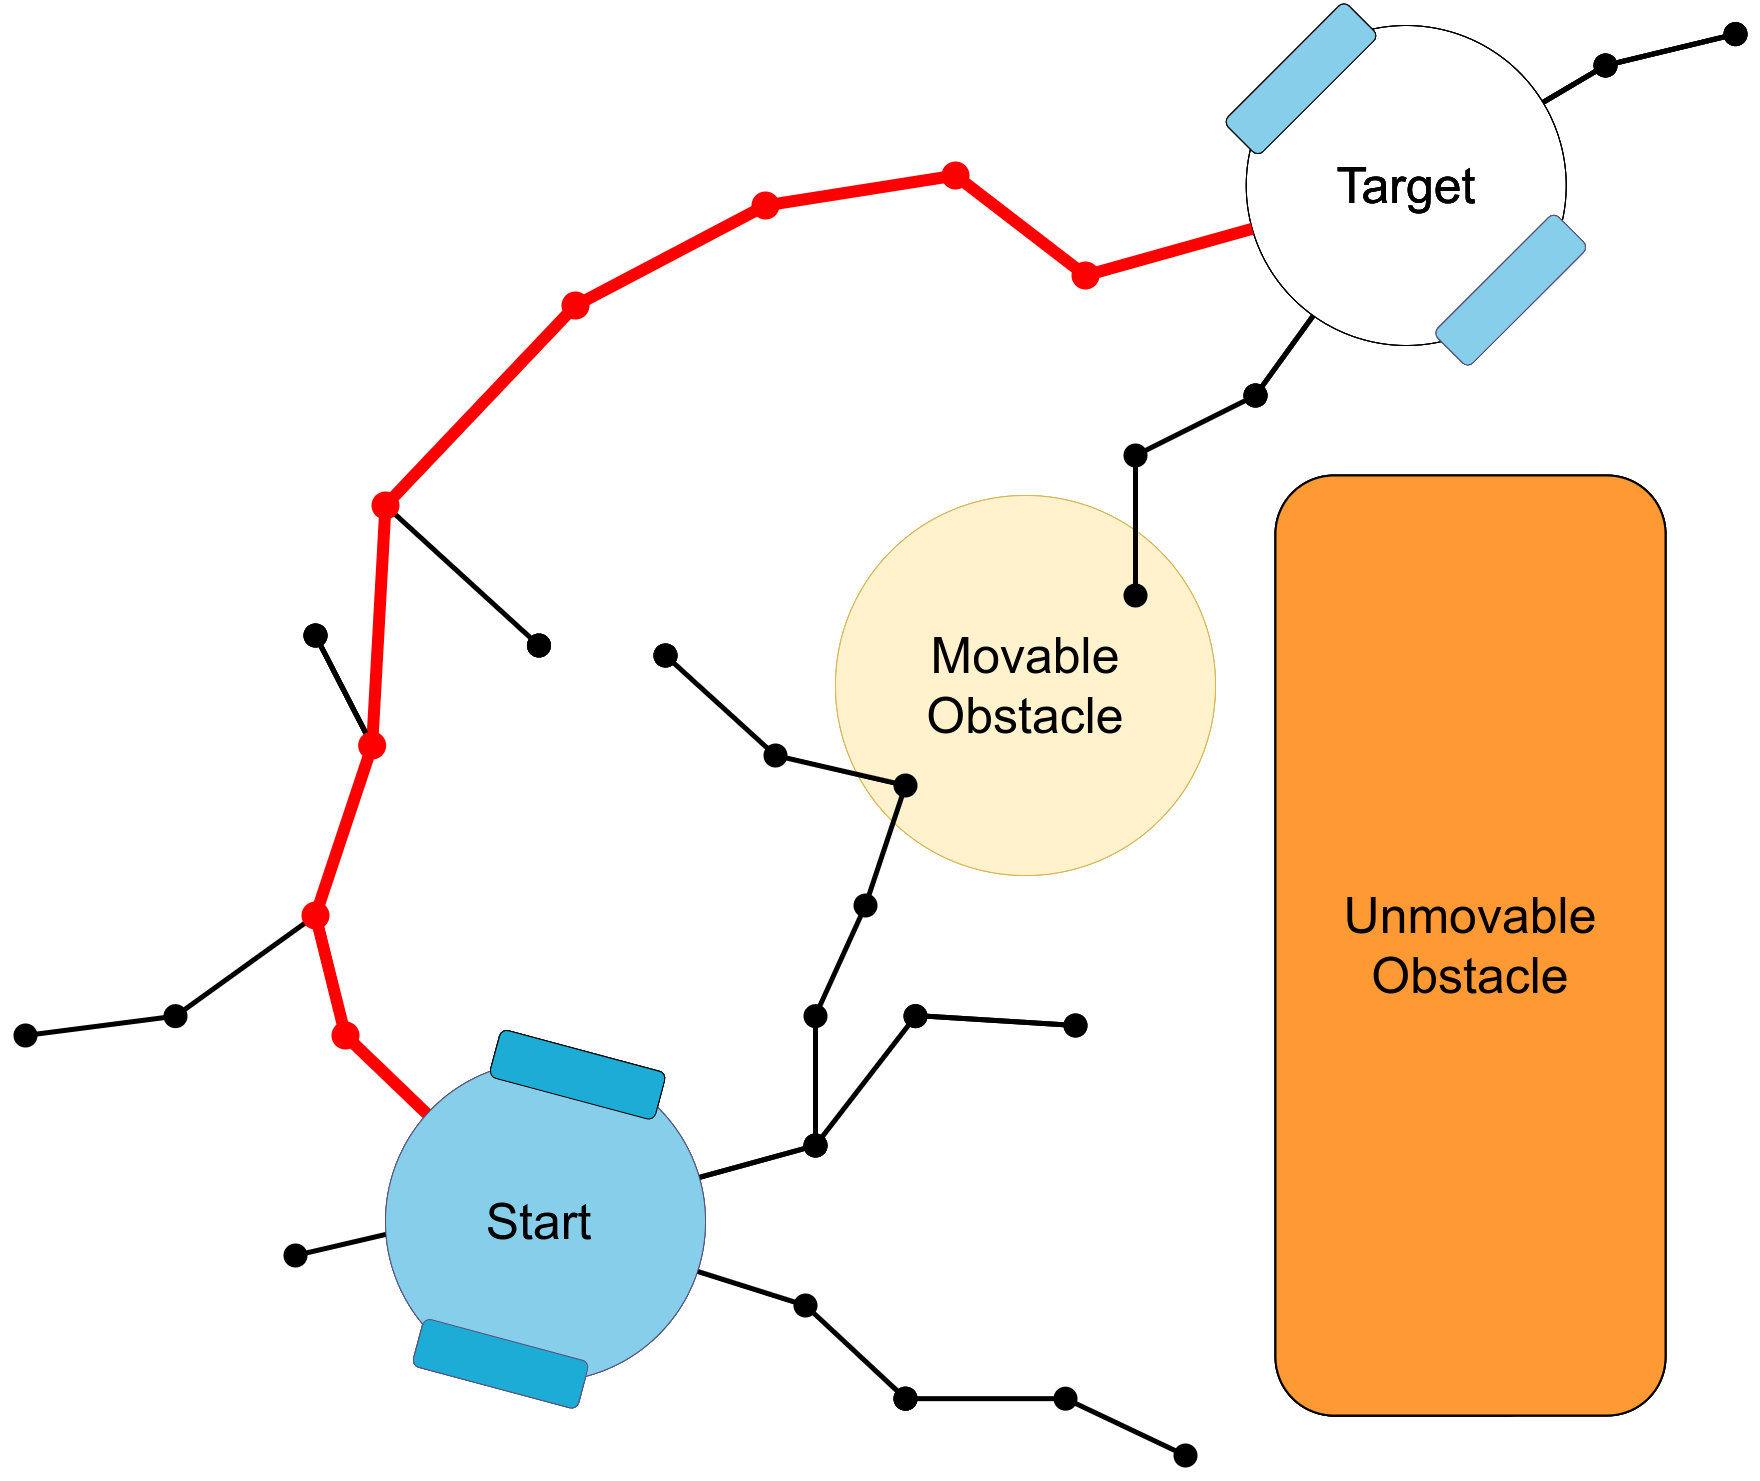
\includegraphics[width=0.8\textwidth]{figures/mp/7mp_path_found.drawio.png}
    \caption{The resulting configuration space after sample in \cref{fig:motion_planner_adding_one_sample}\\ was added. The path found is marked in red}
    \end{subfigure}%
    \begin{subfigure}{.5\textwidth}
    \hspace{-1cm}
    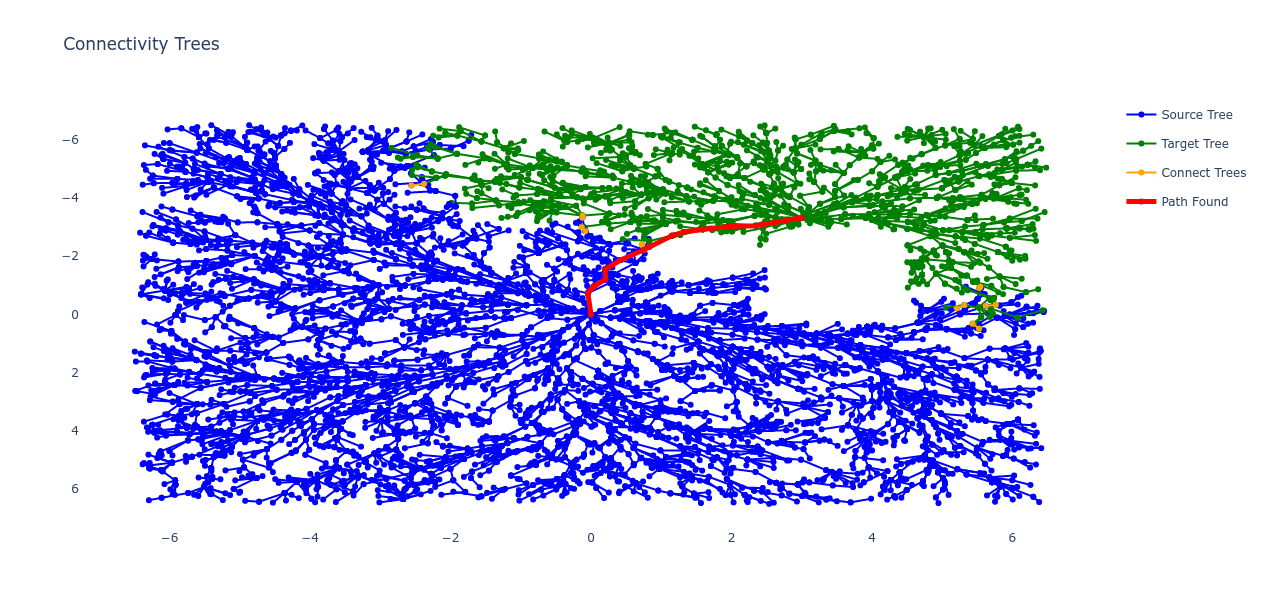
\includegraphics[width=1.1\textwidth]{figures/mp/mp_the_real_deal.png}
    \caption{A visualisation of the implemented \acs{RRT*} algorithm\\after a search from start to target}
    \end{subfigure}
    \label{fig:motion_planner_comparison}%
    \caption{Comparing schematic example to a visualisation of the real algorithm.}
\end{figure}

The result of adding an extra penalty for crossing unknown or movable subspace is that such subspaces are avoided if possible. If it is not possible to find a valid path, then movable or unknown subspaces are crossed, displayed in~\cref{fig:double_rrt_alg}. A path cannot be tracked by a controller if it crosses movable or unknown spaces, first the object must be moved, then the original path can be tracked. In~\cref{fig:double_rrt_alg} it can be seen that the motion planner cannot find a path around the movable object and is forced to add the cost to move the object. The added fixed cost for a path crossing through a movable or unknown objects motivates the motion planner to find the shortest path around objects but prefers moving an object over making a large detour.\bs

\begin{figure}[H]
    \centering
    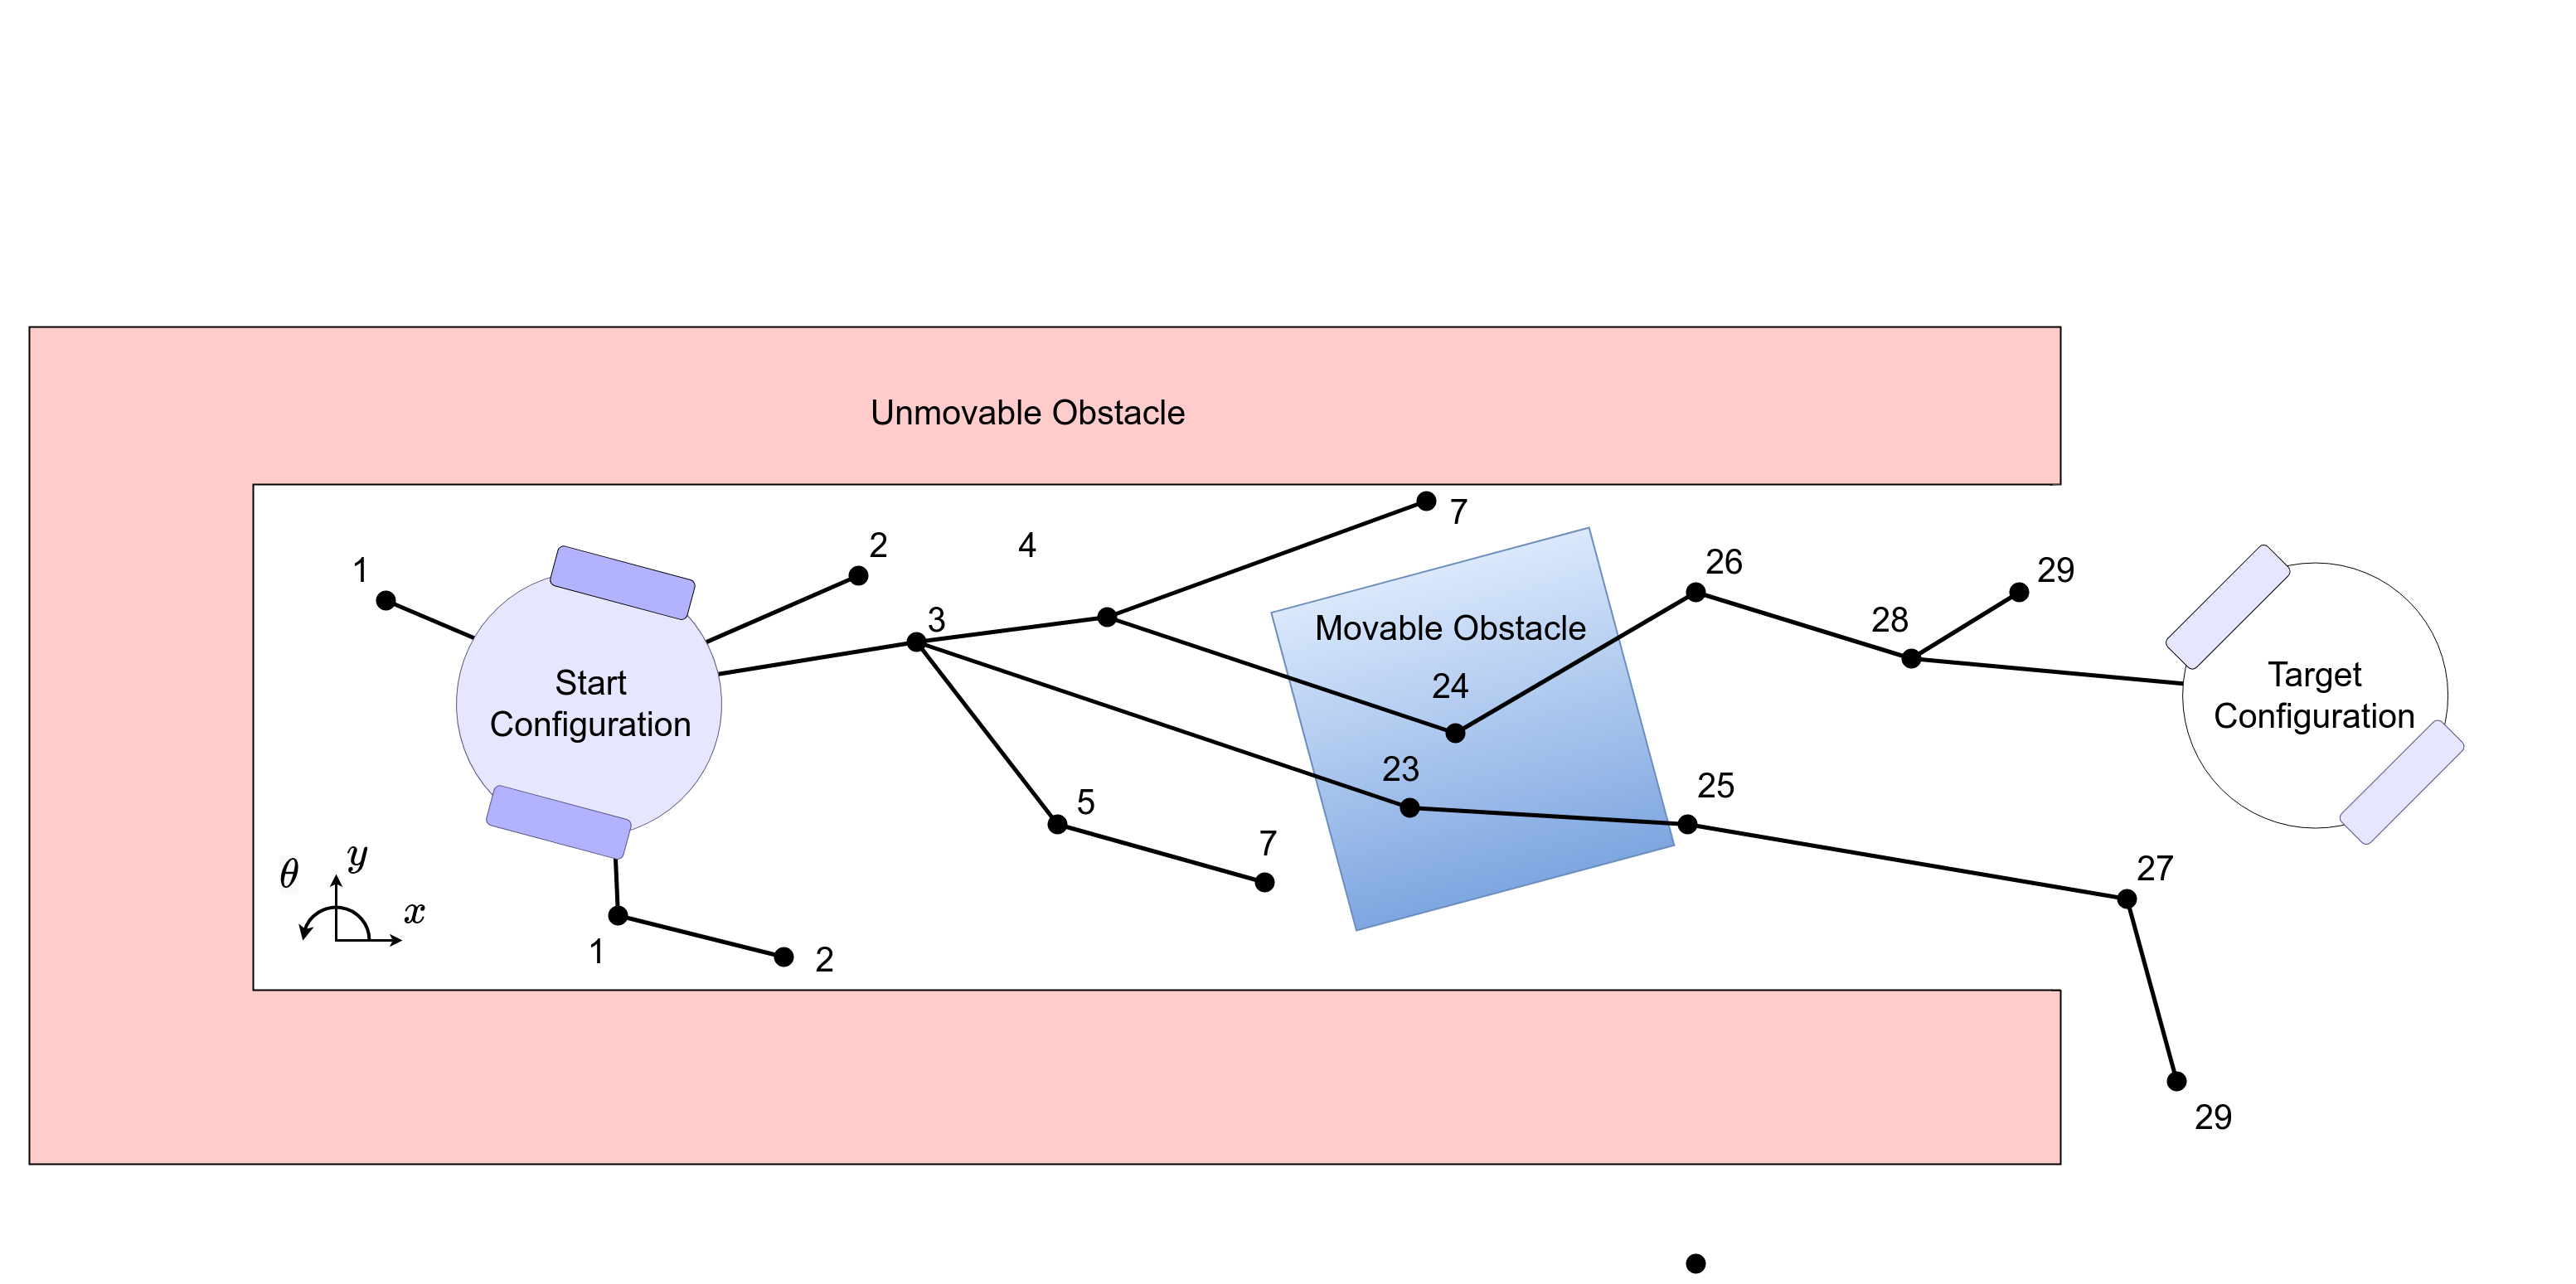
\includegraphics[width=0.9\textwidth]{figures/rrt_with_costs.png}
    \caption{Schematic view of the proposed double $\text{RRT}^*$ tree taking movable and\\unknown objects into account with cost to reach a sampled configuration displayed.}
    \label{fig:double_rrt_alg}
\end{figure}

The proposed motion planning algorithm searches the configuration space from from the start connectivity tree and the target connectivity tree. Exploring faster compared to the single tree \ac{RRT*} algorithm. The proposed algorithm rewires nodes, resulting in lowering the cost for existing paths. The proposed algorithm finds the optimal lowest cost path with infinite sampling because of it's ability to rewire nodes. The $LocalPlannerCheck$ provides paths which are feasible, such that the proposed algorithm yields paths that respect the system constraints. After all later on the system will be controlled to track the path. Now motion planning is discussed, manipulation will be discussed.


\section{Toward an Sequence of Target Poses}
\label{section: toward_sequence_target_poses}
In previous section motion and manipulation planning, planning for a single action was discussed, feasibility of a path depends on local planners in the form of predictors provided by system models discussed in \cref{chapter: interaction_with_env_and_model_identification}. In this section planning for a longer horizon is discussed, \textit{task planning}. As a reminder, a task was defined as a set of objects with associated target configurations. Task planning is defined as the following arisen problem. When given a task, which actions should successfully be performed and in which order to fulfil the given task. Finding such an action sequence in an environment with movable obstacles bears the name \ac{NAMO}. An example is given in \cref{figure: example_task_planning} and serves to clarify the planning problem. In this example the robot is tasked with placing the cube on the location where the sphere currently is.\\

A possible action sequence manually derived would be:\\

\begin{enumerate}
\item drive toward the ball
    \item if no system model is available, perform system identification on the ball
    \item push the ball away such that the box's target position is free 
    \item drive toward the cube
    \item perform system identification on the cube 
    \item push the cube to the target location
    \end{enumerate}
    
\begin{figure}[H]
    \centering
    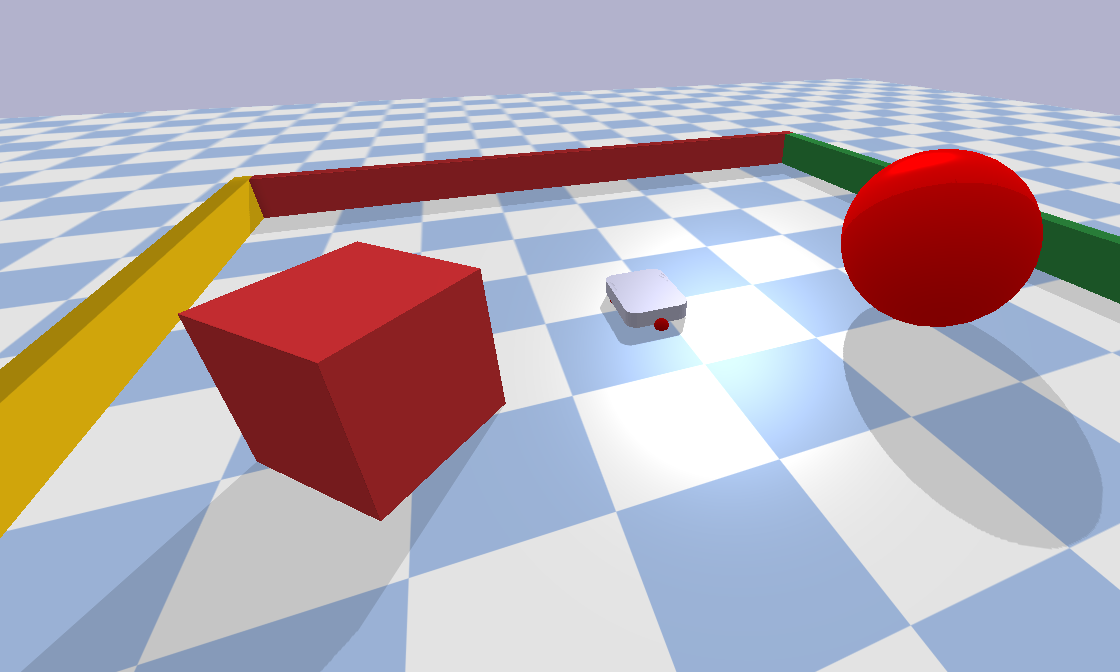
\includegraphics[width=0.6\textwidth]{figures/task_swap_location_balls.png}
    \caption{Example environment with robot, a sphere- and cube object and unmovable walls. The robot is tasked with pushing the cube to the location where the sphere currently is }
  \label{figure: example_task_planning}
\end{figure}

Essentially the task planners job is to create an action sequence, containing subtasks in a logical order which fulfils a larger given task. The task planners reviewed in this literature study fall in to one of the 3 categories: a high-level planners, planning in a joint configuration space and hierarchical planners. Task planners can validate a single motion by querying a motion planning algorithm, discussed in \cref{subsection: motion_planning}. Motion planning algorithms can be queried resulting in a path or the message a path cannot be found, from the perspective of the task planner it appears thus that motion planning is decidable even though it may sometimes given an incorrect answer. 

\subsection{Arisen Problems with Task Planning with Movable Obstacles}
\label{subsection: problems_with_task_planning}
Before diving into arisen problems, the joint configuration space and the piecewise-analytic configuration space are defined. A \textit{joint configuration space} of the robot and the obstacles is created by augmenting the robot configuration space with every configuration space for all objects. For example, if the configuration space for both robot and objects consist of position $X$, $Y$ and orientation $\theta$, then the joint configuration space is $3n$-dimensional, where $n$ is the number of objects including the robot. When the robot manipulates an object, certain multi-body constraints are applicable and are different from single-body constraints, a configuration space containing multiple modes where different constraints apply is called an \textit{piecewise-analytic} configuration space \cite{goldberg_asymptotically_2020}. The joint configuration space with multiple modes of dynamics is an example of a piecewise-analytic configuration space.\\

In this literature, the task planner must solve a \ac{NAMO} problem with unknown but learnable true dynamics. Directly planning in joint configuration space of the robot and objects is tedious for \ac{NAMO} because of different modes of dynamics. For example, the robot can be driving, then pushing and then driving. The push action influences the free space where the robot has to drive in if the push manipulation has ceased. With multiple objects, directly planning in a joint configuration space causes a exponential number of possibilities. \\

With a given task, the target poses of certain objects are given, but that does not specify the location of other objects which may be present in the environment, such as the location of the sphere in the example displayed in \cref{figure: example_task_planning}. If the final positions of some objects are unspecified, this leads to problem dimensionality that is exponential in the number of objects with unspecified target positions in the environment \cite{scholz_navigation_2016}, and is known to be NP-hard \cite{reif_motion_1985}.\\

The two reasons above are indicating the challenges an task planner is facing when solving the \ac{NAMO} problems, both planning in a piecewise-analytic configuration space and trying to solve an NP-hard problem also occur with known dynamics. This literature assumes unknown objects, single-body systems dynamics are a priori not or party known, a priori the dynamics of multi-body systems are unknown. Thus planning has to be performed with learned dynamics which is important to keep in mind, because of estimations of the true dynamics motion and manipulation planning might return unfeasible paths, and feasible paths might not be found. Compared to known dynamics, learned dynamics adds a large layer of uncertainty to the \ac{NAMO} problem.\\

\subsection{Planning in Joint Configuration Space}
\label{subsection: planning_in_joint_config}
As already indicated in \cref{subsection: problems_with_task_planning}, the joint configuration space's dimensionality grows linearly, meaning the joint configuration space grows exponentially in the number of objects, which is an explosion in the number of possible combinations the environment can be in. Even sampling cannot computationally find a path in reasonable time, only by leveraging simplifications a search be performed. The upcoming solutions to search in the joint configuration space all implement some simplification to prevent sampling the entire joint configuration space. \\

Note that while other task planning methods might use motion/manipulation planning to validate motions/manipulations, planning in joint configuration space does not. Planning in joint configuration space essentially is motion/manipulation planning for a longer horizon than a single action.\\

Novin \cite{sabbagh_novin_optimal_2016} develops a task planner for the \ac{NAMO} problem combined with placing objects on target positions which is capable of finding a local minimum in the joint configuration space. Tackling the combinational explosion using 2 different tactics, first, a disjunctive programming concept is applied to convert the continuous problem to discrete form, where a continuous path is equivalent to some points with equal time distance in between, second, a heuristic function is implemented, which allows for planning toward the goal for a fixed number of time steps. Such a receding horizon allows only to search a path close to the current joint configurations. Planning toward configurations lowering a metric function indicating the direction toward the final target configuration. Convex optimisation then finds an optimal path regarding the considered horizon \cite{sabbagh_novin_optimal_2016}. Novin then finds the \ac{NAMO} problem while learning dynamical properties in a hospital setting. Where patients are assisted by the patients' assistant mobile robot which can move obstacles out of the way or hand patients their walker. In addition to the task planner, a Bayesian regression algorithm was used to estimate the object dynamical model and an \ac{MPC}-based controller was used to follow a specified path \cite{novin_dynamic_2018}. In a follow-up paper, trajectory errors have been lowered and the selection of objects to encounter has been enlarged \cite{sabbagh_novin_model_2021}. Novin has shown that by sampling close to the current configuration, a path can be found in high dimensional configuration spaces in reasonable time. The patient assistant mobile robot is able to find and track a path in real-time.\\

\cite{goldberg_asymptotically_2020} solves the \ac{NAMO} problem by first extending existing algorithms developed by \cite{hauser_randomized_2011} to an optimal but prohibitively computationally expensive algorithm. Then the configuration space is factored while preserving optimality, this reduces the complexity considerably, by considering only a finite collection of subsets of the configuration space, each of which is subject only to analytic constraints. By building a graph on each of these subsets and connecting the resulting collection of graphs, we can construct a random graph that spans the configuration space. As the collection grows sufficiently large, it will contain a near-optimal plan with probability one and an optimal plan in the limit of infinite samples. \\

The 2 papers discussed have shown that the computational nightmare of the joint configuration space can be tamed by techniques such as discretization, factorization or a heuristic function combined with a time horizon. Such techniques prevent searching in configurations relatively far from the current configuration, while optimality guarantees can be given and real-time implementations have been shown. A relief bonus for solving the \ac{NAMO} problem in the joint configuration space which requires much computation power is that it removes the need for individual motion or manipulation planning. It can be concluded that if clever techniques keep the dimensionality to an reasonable small subspace, such that the robot can start tracking a path in under a minute of searching, path searching in the joint configurations space is a successful methods for task planning.\\

\subsection{High-level Planners}
\label{subsection: high_level_planners}
\textit{High-level planners}, in this literature refers to an ontology defining the structure of knowledge in a certain domain and a planner which when queried with a task or question uses the ontology to derive an answer or action sequence. Advanced high-level planners automatically try to satisfy 'logical' constraints that for humans feel obvious such as holding a cup upright if it is filled with liquid. A summary of high-level languages, planners and frameworks specialised for robotic applications will now be discussed, for this discussion, the literature study of M. Mâachou has been used containing a recent summary of the high-level planners \cite{maachou_mohommed_knowledge-based_2021}. \\

Note not all high-level planners \textit{must} use an \textit{ontology}, many however do, to categorise objects and actions as concepts, roles and instances. An example concept is the set of mobile robots with grippers, Tiago (a mobile robot with grippers) is an instance of the concept mobile robots with grippers, $\text{apple}_1$ is an instance of the concept fruit and can be gripped by Tiago, then the role Tiago.canGrab($\text{apple}_1$) indicates that Tiago can grab $\text{apple}_1$. Ontologies create hierarchical categorisations for example, a categorisation of products in a supermarket where chocolate croissant is a subconcept croissant, a subconcept of bread. Most popular languages to store an ontologies are the \ac{PDDL} and the \ac{OWL}. Ontologies cannot categorise and relate every action, concept or physical object existing in the real world, that is way too much data. That is why ontologies are specific to a certain domain such as a supermarket environment, an hospital environment or a family home. Large domain-specific ontologies are available open-source, for robotics applications the most popular ontologies are \ac{SUMO}, \ac{CORA} and \ac{DOLCE}. \\

Ontologies are deterministic, the closed-world assumption (note, not the same assumption as assumption \ref{assumption: closed_world}) is used to make unknown statements decidable, the closed-world assumption states, anything not known to be true is assumed to be false. While learning dynamical properties many statements are unknown, with the closed-world assumption high-level planners mainly would assume manipulation to be impossible, for example, if the high-level planner is queried with "can the unknown object be moved", the answer would simply lead to false because it is unknown. Here \textit{affordances} can help to make an estimation, affordance is defined as the ability to perform a certain action with an object in a given environment \cite{ardon_affordances_2020}. Concluding that a certain manipulation action would lead to success with an unknown object requires some experience before any conclusion can be drawn. Actions which collect experience for a given object should be triggered in high-level planners to update the knowledge base which then bypasses the closed-world assumption. \\

Frameworks (which include a ontology, planner and more) such as KnowRob \cite{beetz_know_2018} or the perception and manipulation knowledge  \cite{diab_pmkknowledge_2019} show the effectiveness of high-level planners in robotic applications. \\

High-level planners in practice are successful in generating an action sequences, however, in the scope of this literature study, where tasks are defined as a set of objects with target configurations high-level planners are not needed. There is not classification of objects required, no distinction between physical places such as kitchen and living room. An high-level planner in the scope of this literature is thus overkill. Simple heuristic and flowchart like decisions trees, see \cref{figure: navigation_algorithm} achieve the same performance as expensive planners, thus the former is preferred. 

\begin{figure} \centering
\begin{tikzpicture}[node distance = 2cm, auto]
    % Place nodes
    \node [block] (global) {Global Path};
    \node [decision, below of=global] (obstacle) {Obstacle Detected};
    \node [block, below of=obstacle, node distance=3cm] (generate) {Generate Obstacle};
    \node [decision, below of=generate] (movable) {Movable};
    \node [block,  left of=movable, node distance=3cm] (remove) {Remove Obstacle};
    \node [block,  right of=movable, node distance=3cm] (replan) {Replan Path};
    % Draw edges
    \path [line] (global) -- (obstacle);
    \path [line] (obstacle) --  node [near start] {yes} (generate);
    \path [line] (obstacle.west) -| ($(obstacle.west) - (1,0mm)$) |-  node [near start] {no} (global.west);
    \path [line] (generate) -- (movable);
    \path [line] (movable) --  node [near start, above] {yes} (remove);
    \path [line] (movable) --  node [near start] {no} (replan);
    \path [line] (remove) |- (global);
    \path [line] (replan) |- (global);
\end{tikzpicture}
\caption{Flowchart representation of navigation algorithm \cite{wang_affordance-based_2020}}
\label{figure: navigation_algorithm}
\end{figure}


\subsection{Hierarchical Planning}
\label{subsection: hierarchical_planning}
Hierarchical planners separate the robot's configurations space into subspaces. In such graphs where the subspace is a section where a single dynamical mode holds true, such as driving, pulling or pushing. During seperations into subspaces, actions are generated and a graph (such as a \ac{MDP} or search tree \cite{bronson_practical_2010}) combines actions with subspaces, where the nodes correspond to robot and object poses, and transitions to actions. Solving a task planning problem is then defined as finding a list of transitions which start in the current configuration (contained inside a subspace) and end in the target configuration (inside a subspace), an example is displayed in \cref{figure: example_hierarchical_planning}.\\

\begin{figure}[!h]
    \centering
    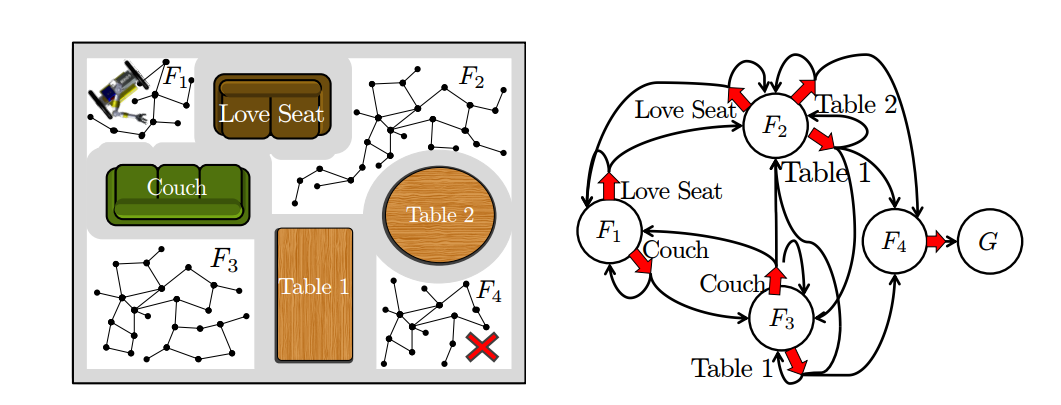
\includegraphics[width=0.9\textwidth]{figures/construct_hierarchical_planner.png}
    \caption{Schematic overview of the robots' free space separated is subgraps in \acs{PRM} and the corresponding \acs{MDP}, from \cite{scholz_navigation_2016}
    }
    \label{figure: example_hierarchical_planning}
\end{figure}

\Cref{figure: example_hierarchical_planning} displays a schematic overview of a separated configuration space of the robot, free space is made into 4 subspaces, $F_1$, $F_2$, $F_3$ and $F_4$. Detecting subspaces is found by finding disconnected connectivity graphs after a limited number of samples, and objects inbetween disconnected graphs can be extracted based on position relative to the sampled configurations. An \ac{MDP} can then be constructed and is viewed as a reward shaping mechanism to focus the low-level search on actions that are likely to clear paths to useful locations \cite{scholz_navigation_2016}. Solving the \ac{MDP} generates multiple ordered action sequences which would lead to the robot's target configuration. \\

Task planning with learned dynamics was first done by Scholz \cite{scholz_navigation_2016}, the work has inspired \cref{figure: example_hierarchical_planning} and it was the first attempt to solve the \ac{NAMO} using learned dynamics \cite{scholz_learning_2015}.  By using a hierarchical \ac{MDP} formulation of the \ac{NAMO} problem designed to handle dynamics uncertainty, Scholz successfully demonstrated the ability of a robot to adapt to unexpected object behaviour such as a table which upon inspection turned out to be unmovable. A key difference between Scholz task description and this literture review's task description is that in \cite{scholz_navigation_2016} the target position for only the robot is given, where as this literature includes possibly some target positions for objects. Including target positions for the obstacles makes such a problem quite a bit harder since additional planning is required, it is then unclear if such a problem can be solved using sampling algorithms combined with an \acp{MDP}.\\

Instead of defining actions and subgraphs as previously shown, \textit{backward induction} determines the actions, and applies them to the target configuration to search for the starting configuration. An arisen problem is the unspecified target positions of the objects in the environment. A workaround is to simplify the \ac{NAMO} problem to object rearrangement for which all start and target configurations are specified. Krontiris and Bekris created such conditions in object rearrangement problem in which object move over a straight line, and can only be moved once (monotone problem) \cite{krontiris_dealing_2015}. A graph is created where nodes corresponding to the objects pose in the world. From target node to the current node is searched in a backwards fashion. With the monotone rearrangement search algorithm constructed by \cite{krontiris_dealing_2015} finding a solution is sublinear in the number of objects to rearrange and the algorithm is run-time applicable. \\

Generally target positions other than the robot itself are not specified in \ac{NAMO} problems. Unspecified target positions can be randomly chosen, as \cite{siciliano_path_2009} has shown. By augmenting a search tree with manipulated objects to random locations, a special feature is that \cite{siciliano_path_2009} keeps track of the robot and object configurations within the search tree. Randomly selected actions applied to randomly chosen actions guarantees probabilistic completeness for infinite sampling, but the computational power required increases drastically with the size of the number of objects and size of the workspace (and thus directly configurations space). Heuristic functions could potentially prevent unnessecary sampling into unrelevant subspaces of the configuration space, such as \cite{sabbagh_novin_model_2021} has shown.\\

Heuristic task planners find solutions which are \textit{hierarchical}, they will return the best feasible plan that can be expressed within the task hierarchy they search \cite{goldberg_asymptotically_2020}. System models contain some model mismatch with the true dynamics. Both the hierarchical solutions and effects of model mismatch are acceptable mainly because the \ac{NAMO} problem is NP-hard. Hierarchical planners are relatively computationally efficient, compared to planning in joint configuration space and find a action sequence (even though that might be hierarchical). It can be concluded that hierarchical planners are thus a right fit to determine action sequences in the scope of this literature. \\

\section{Discussion}
\label{section: tamp_discussion}
sample- and graph based motion and manipulation planning algorithms have been discussed, the most applicable motion planning algorithms are the sample-based algorithms because they can search high dimensional spaces efficiently compared to graph-based planners. a connectivity graph build on sampled configurations indicates if samples are reachable from other sampled configurations while satisfying constraints imposed by the local planner. Feasibility has been shown to depend on local planners, who's accuracy directly depends on system models discussed in previous chapter. both path existence and convergence properties have been discussed, which allows to conclude that sample-based planners can efficiently search for motion and manipulation problems, additional checks such as path existence can speed up arriving to conclusions, such as "no path exists". \\

The joint configuration space is a piecewise-analytic configuration space containing multiple modes of dynamics. Because this joint configuration space dimensionality grows linearly (and the configurations space thus exponentially) with the number of objects, it is computationally infeasible to search for a path. Especially considering that with robotic application  solutions found in real-time are highly appreciated. The exponentially fast growing joint configuration space is an answer to the second research subquestion. \\

Three main methods have been discussed to determine an action sequence to reach a given task, firstly planning in a joint configuration space where the dimensionality grows so enormously fast that measures have to be taken in order to make the problem computable. Using techniques such as discretisation, a finite planning horizon or factorisation decrease the search space such that real-time planning is possible, allowing to conclude that planning in joint configuration space is effective, and applicable for task planning with learned dynamics. Secondly, high-level planners, which with an ontology and planner determine an action sequence. The task is defined as a set of object and corresponding target configurations, this form of task and the lack of categorisation of objects yields high-level planners shy of providing effective solution. To conclude high-level planners are not fit for determining a action sequence in this literature. The last methods is hierarchical planning, by seperating the joint configuration space in local subspace where one mode of dynamics holds, motion planning algorithms can find a paths in these subspaces, a global plan is found by generating a search tree or \ac{MDP} from planning to target. The solutions found are hierarchical, which limits converging to a global minimum, even so the methods is efficient compared to a search into joint configuration space. With learned, possibly inaccurate dynamical models, converging toward the optimal path is not the goal of the task planner, and hierarchical solutions with computational efficiency are preferred, allowing to conclude that hierarchical solutions are effective and applicable approach to find an action sequence for tasks to execute in an environment with movable obstacles.\\ 

\chapter{Proposed Method}
\label{chapter: proposed_method}
\textit{The goal of this chapter is to provide a description of the proposed algorithm and to list tests with expected outcomes which, if implemented provide evidence for the effectiveness of the algorithm. The previous chapter has answered the first 2 research subquestions by showing existing methods and their limitations which have been highlighted. This chapter answers the last research subquestion by providing a draft method to be investigated in the thesis, the method can complete tasks while learning system dynamics during task execution in an environment with movable obstacles. The proposed algorithm relies on many existing methods which have been discussed in \cref{chapter: interaction_with_env_and_model_identification,chapter: task_and_motion_planning} and will be rediscussed briefly in \cref{subsection: required_components}. \Cref{section: hgraph} defines the hypothesis graph, as \cref{section: knowledge_graph} defines the knowledge graph. Benchmark tests are listed in \cref{section: btests}. The Discussion is presented in \cref{section: proposed_method_discussion}.\\}

In this literature study the focus lies on the knowledge graph (KGraph), the hypothesis graph (HGraph) and the robot simulation environment. If the literature study focus would be complemented with a high-level planner and an ontology, the robot framework would be theoretically capable of handling high-level tasks, such as grouping objects based on shape, or cleaning.\\

\textbf{\large general outline\\}
\noindent \Cref{figure: block_framework} displays the general outline control structure for the robot. Upon receiving a task, the \textit{hypothesis graph} is responsible for generating a hypothesis, an action sequence which might lead to successful completion of the given task. Replanning may occur after learning objects are immovable or when control fails to complete a subtask, if all possible hypothesis have been tried, then HGraph concludes that the task cannot be done. \Cref{section: hgraph} is fully dedicated to explaining the hypothesis graph.\\

After execution of an action, the action is evaluated and newly learned knowledge is stored or updated in the \textit{knowledge graph}. Aside from storing knowledge, the knowledge graph provides action suggestions to the hypothesis graph. \cref{section: knowledge_graph} is fully dedicated to explaining the knowledge graph.\\

\begin{figure}[H] \centering
\begin{tikzpicture}[node distance = 2cm, auto]
    % Place nodes
    \node[draw=gray, rounded corners, inner sep=3ex, line width=7pt, fill=gray, fill opacity=0.4, minimum height=12.1cm, minimum width=6.8cm, yshift=3.7cm] (focusbox) {}; 
    \node[yshift=5.5cm, xshift=-0.6cm, align=left] at (focusbox) {\textbf{Literature study focus}};
   
   \node [outer sep=0cm] (environment) at (0,0)  {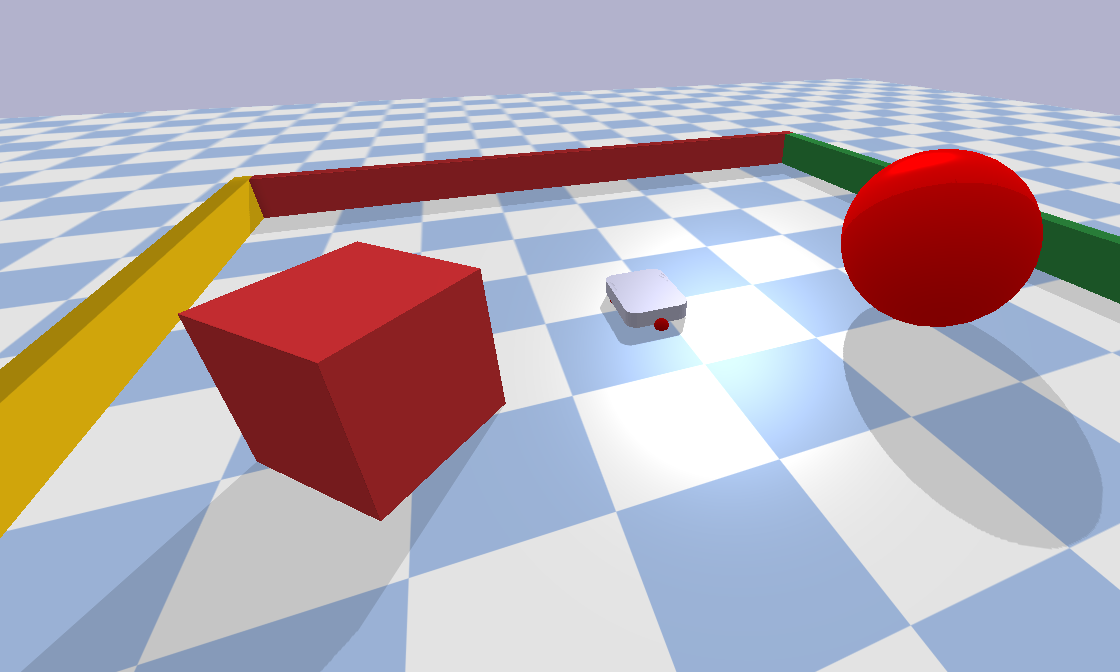
\includegraphics[width=5.0cm]{figures/task_swap_location_balls.png}}; 

   \node [below, xshift=0.2cm, yshift=-.1cm, text width=5cm, align=left, outer sep=0cm] at (environment.north) {\textbf{Robot Environement}};
   
    \draw [myEvenLighterColor,
    rounded corners=0.3cm, 
    line width=0.3cm]  
    (environment.north west) -- 
    (environment.north east) --
    (environment.south east) --
    (environment.south west) -- cycle  ;
    
    \node [block,
    above of=environment,
    minimum height=2cm,
    minimum width=5cm,
    node distance=4.3cm,
    outer sep=0cm] (hgraph) {Hypothesis Algorithm};
   
    \node [block, 
    above of=hgraph, 
    node distance=3.5cm, 
    minimum width=5cm,
    minimum height=2.0cm] (kgraph) {Knowledge Graph};
      
    \node [rectangle, draw, 
    fill=myEvenLighterColor, 
    text width=5em, text centered, rounded corners, 
    right of=kgraph, 
    minimum width=4cm,
    minimum height=2cm,
    node distance=8cm] (ontology) {Ontology};
     
    \node [rectangle, draw, 
    fill=myEvenLighterColor, 
    text width=5em, text centered, rounded corners, 
    right of=hgraph, 
    minimum width=4cm,
    minimum height=2cm,
    node distance=8cm] (planner) {High-level planner};
    
    
    % Draw edges
    \draw[-stealth] ([yshift=0.155cm, xshift=0.4 cm]environment.north) -- node [right] {\shortstack[]{sensor\\measurements}}([xshift=0.4 cm]hgraph.south) ;
    \draw[-stealth] ([xshift=-0.4 cm]hgraph.south) -- node [left] {robot input}([yshift=0.155cm, xshift=-0.4 cm]environment.north) ;
    \draw[-stealth] (planner.west) -- node [pos=0.37, above] {task}(hgraph.east);
    \draw[-stealth] ([xshift=-0.4cm]kgraph.south) -- node [left] {\shortstack[]{action\\suggestions}}([xshift= -0.4cm]hgraph.north) ;
    \draw[stealth-] ([xshift=0.4cm]kgraph.south) -- node [right] {action feedback}([xshift= 0.4cm]hgraph.north) ;
    \draw[-stealth] (kgraph.east) -- node [above, pos=0.63] {\shortstack[]{environment\\knowledge}}(ontology.west);
    \draw[stealth-] ([xshift=0.4cm]ontology.south) -- node [right] {\shortstack[]{query}}([xshift=0.4cm]planner.north);
    \draw[-stealth] ([xshift=-0.4cm]ontology.south) -- node [left] {\shortstack[]{output}}([xshift=-0.4cm]planner.north);
    \draw[stealth-] (planner.south) |- ++ (2,-1) node[near end, above] {\shortstack[]{High-level\\task}};
    \end{tikzpicture}%
    
\caption{Complete control scheme in Flowchart representation.}
\label{figure: block_framework}
\end{figure}

\section{Required Components}
\label{subsection: required_components}
% yes the label says subsection, it actually is a section
This section lists required components used by the proposed method, such as: path-finding algorithms, controllers or system identification methods. The required components are neatly grouped in this section, every component has a specific citation and it is indicated if any modifications must first be applied before it can be used by the proposed method. The required components are minimally explained, and their function and responsibilities are highlighted. \\

\paragraph{Path Non-Existence}
Before motion planning, the HGraph checks path non-existence, more information on path existence can be found in \cref{subsection: path_existence}. As opposed to motion or manipulation planning two simplifications are made: an obstacle (such as the robot or an environment object) is assumed to be holonomic, and only the unmovable objects are actively present in the configuration space, unknown and movable obstacles are ignored. In configuration space, the free space is discretised with a cell size based on the geometry of the robot or object, a graph-based planner then searches to find a path from starting cell toward the target cell, \cref{figure: path_existence_cite} displays a visual explanation of the path non-existence checker. Paper \cite{akella_simple_2008} describes the method applicable to prove path non-existence, if a path is found toward the target position, the cells containing a path will be converted to sample points in configuration space, serving as a warm start for the motion or manipulation planning algorithms. \\

\begin{figure}[H]
    \centering
    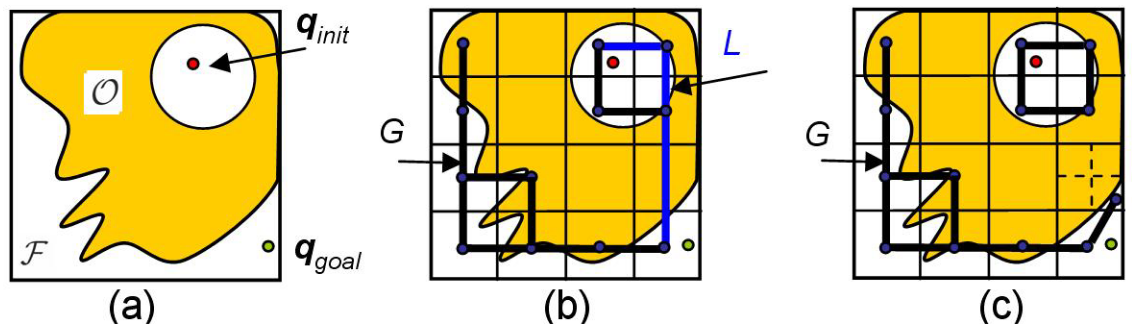
\includegraphics[width=0.8\textwidth]{figures/path_existance_cite.png}
    \caption{Path non-existence between $\text{q}_\text{init}$ and $\text{q}_\text{goal}$. (b): A connectivity graph $G$ is built. The path $L$, which connects the cells including $\text{q}_\text{init}$ and $\text{q}_\text{goal}$, is computed from G. Any mixed cell along $L$ is further subdivided. (c): In the new connectivity graph, the cell containing  $\text{q}_\text{init}$ and the cell containing  $\text{q}_\text{goal}$ are not connected. This concludes that there is no collision-free path between $\text{q}_\text{init}$ and $\text{q}_\text{init}$, From \cite{akella_simple_2008}.}
    \label{figure: path_existence_cite}
\end{figure}

\paragraph{System identification and Control}
In \cref{section: interaction_approaches_and_model_iden_methods} various system identification en control methods have been discussed. Some methods are appropriate candidates for a nonholonomic robot and an environment with movable obstacles. The control and system identification methods are not discussed again here, since they have already been discussed in \cref{section: interaction_approaches_and_model_iden_methods}. The system models generated by system identification methods act as forward models or local planners during motion and manipulation planning as discussed in \cref{section: toward_target_pose,section: toward_sequence_target_poses}.\\
\\

Appropriate candidates for single-body control with system identification methods:
\begin{itemize}
    \item \ac{MPC} control and \ac{PEM} \cite{verhaegen_filtering_2007} system identification
    \item \ac{MPC} control and \ac{IPEM} \cite{seegmiller_vehicle_2013} system identification 
\end{itemize}

A parameterisable system model improves its model accuracy using the \ac{PEM} (offline) or \ac{IPEM} (online) method, the \ac{MPC} controller however keeps constant parameters such as control horizon and the weight matrices. To have some variation in these constant parameters, the robot has access to multiple \ac{MPC} controllers with various control parameters. \\

Appropriate candidates for multi-body system identification and control are:
\begin{itemize}
    \item Reactive \ac{MPC} which requires a single- and multi-body model \cite{toussaint_sequence--constraints_2022}
    \item \ac{MPC} controller and model fitting a 3D-Gaussian \cite{mericli_push-manipulation_2015}
    \item \ac{MPPI} controller and uncertainty calibrated forward model \cite{arruda_uncertainty_2017}
    \item \ac{RMPPI} controller and a \ac{LSTM} \cite{cong_self-adapting_2020}
\end{itemize}

\paragraph{Motion and Manipulation planning}
Finding paths between starting and target configurations is performed by a sampling-based method, a double tree $\text{RRT}^*$ search algorithm \cite{chen_fast_2018}, which searches the configuration space for an optimal path toward the target position. A connectivity graph, (initially only the start and target configuration) keeps track of the configurations reachability from the start and target configuration. Randomly sampled samples are compared to some nearest nodes inside the connectivity graph, before adding the newly sampled node, a check is performed by a local planner to validate if constraints are satisfied, if the random sampled configuration is not valid, it is discarded. The connectivity graph grows from the target configuration and the start configuration, when the connectivity graph from start to target is connected a path is found, pseudocode can be found in \cref{pseudocode: rrt_star}.\\

Manipulation planning is similar to motion planning. With motion planning, planning for the robot is performed, with manipulation planning, planning for the objet to push is performed (and the robot is neglected, but kept track of). So manipulation planning only happens as motion planning for the pushable object.\\

The robot configuration is manipulation planning is kept to validate the reachability to newly sampled samples. To elaborate, adding a new sample is accomplished by, sampling a new configuration for the object to manipulate, the sample is placed in configuration space, with a manually tuned metric function samples nearby the new sample are gathered. A local planner validates if these gathered samples are reachable from the new sample. One configuration is reachable from another configuration if for some input and some system model, one configuration becomes the other configuration in a small amount of time (e.g. $<5$ time steps) an example of such a system model is displayed in \cref{equation: differential_equation_differential_robot}. The difference in predictor between motion (single-body predictor) and manipulation planning (multi-body predictor) thus resides in the local planner and where local motion planner requires 2 configurations, manipulation planning  additionally requires at least one robot configuration. To check if 2 configurations are reachable for manipulation planning 2 object configurations and 1 robot configuration is required, if reachable and connected, an extra robot configuration is generated as a result of the local planner, which is needed for checking reachability of future samples, an visual example is displayed in \cref{figure: local_planner_manipulation}. A manipulation path from start to target will have both the objects and the robot's configurations, where the robot configurations only serve the local planner to validate if two object configurations can be connected. Additionally the robot's path should not collide with obstacles, which needs to be checked during planning. \\

\begin{figure}[H]
    \centering
    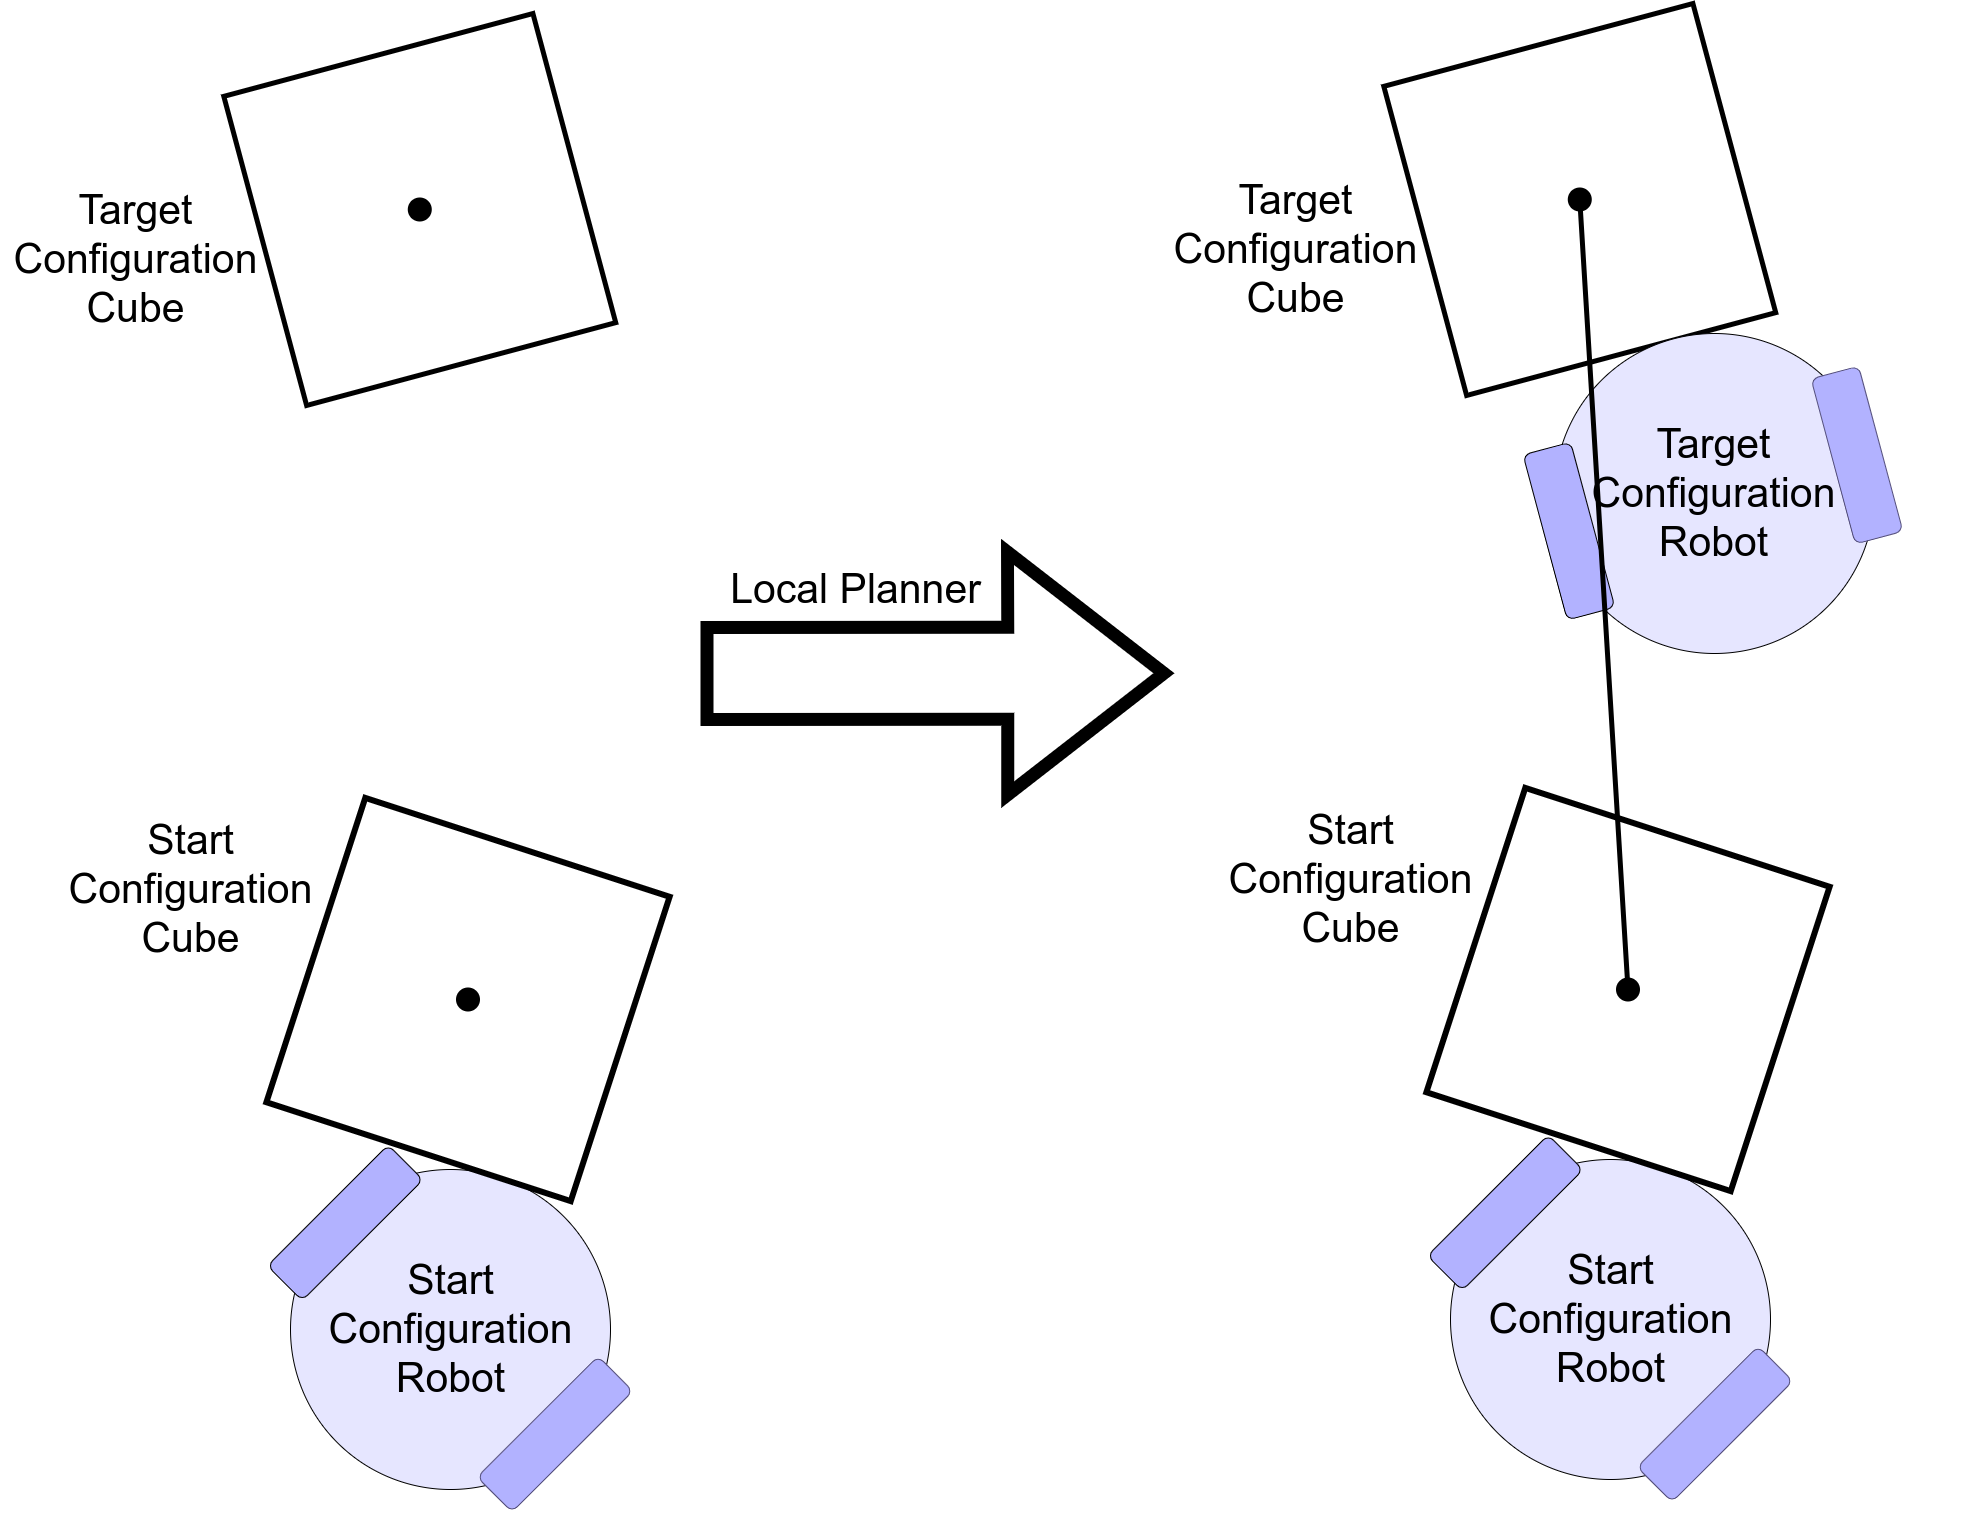
\includegraphics[width=0.7\textwidth]{figures/manipulation_local_planner.png}
    \caption{Local planner connecting 2  cube configurations and generating an new robot configuration}
    \label{figure: local_planner_manipulation}
\end{figure}

The $\text{RRT}^*$ algorithm takes a cost for path length into account, resulting in finding the shortest path with infinite samples if a path exists, an additional cost is added if the path overlaps with a movable or unknown obstacle, motivating the algorithm to find a path around unknown or movable obstacles, but to plan through the obstacles planning around is impossible or costs more. If a path overlaps with an obstacle, a subtask is created to first remove the obstacle, and then continue to track the path. \Cref{figure: double_rrt_alg} gives a visual view of the proposed $\text{RRT}^*$ algorithm.\\

\begin{figure}[H]
    \centering
    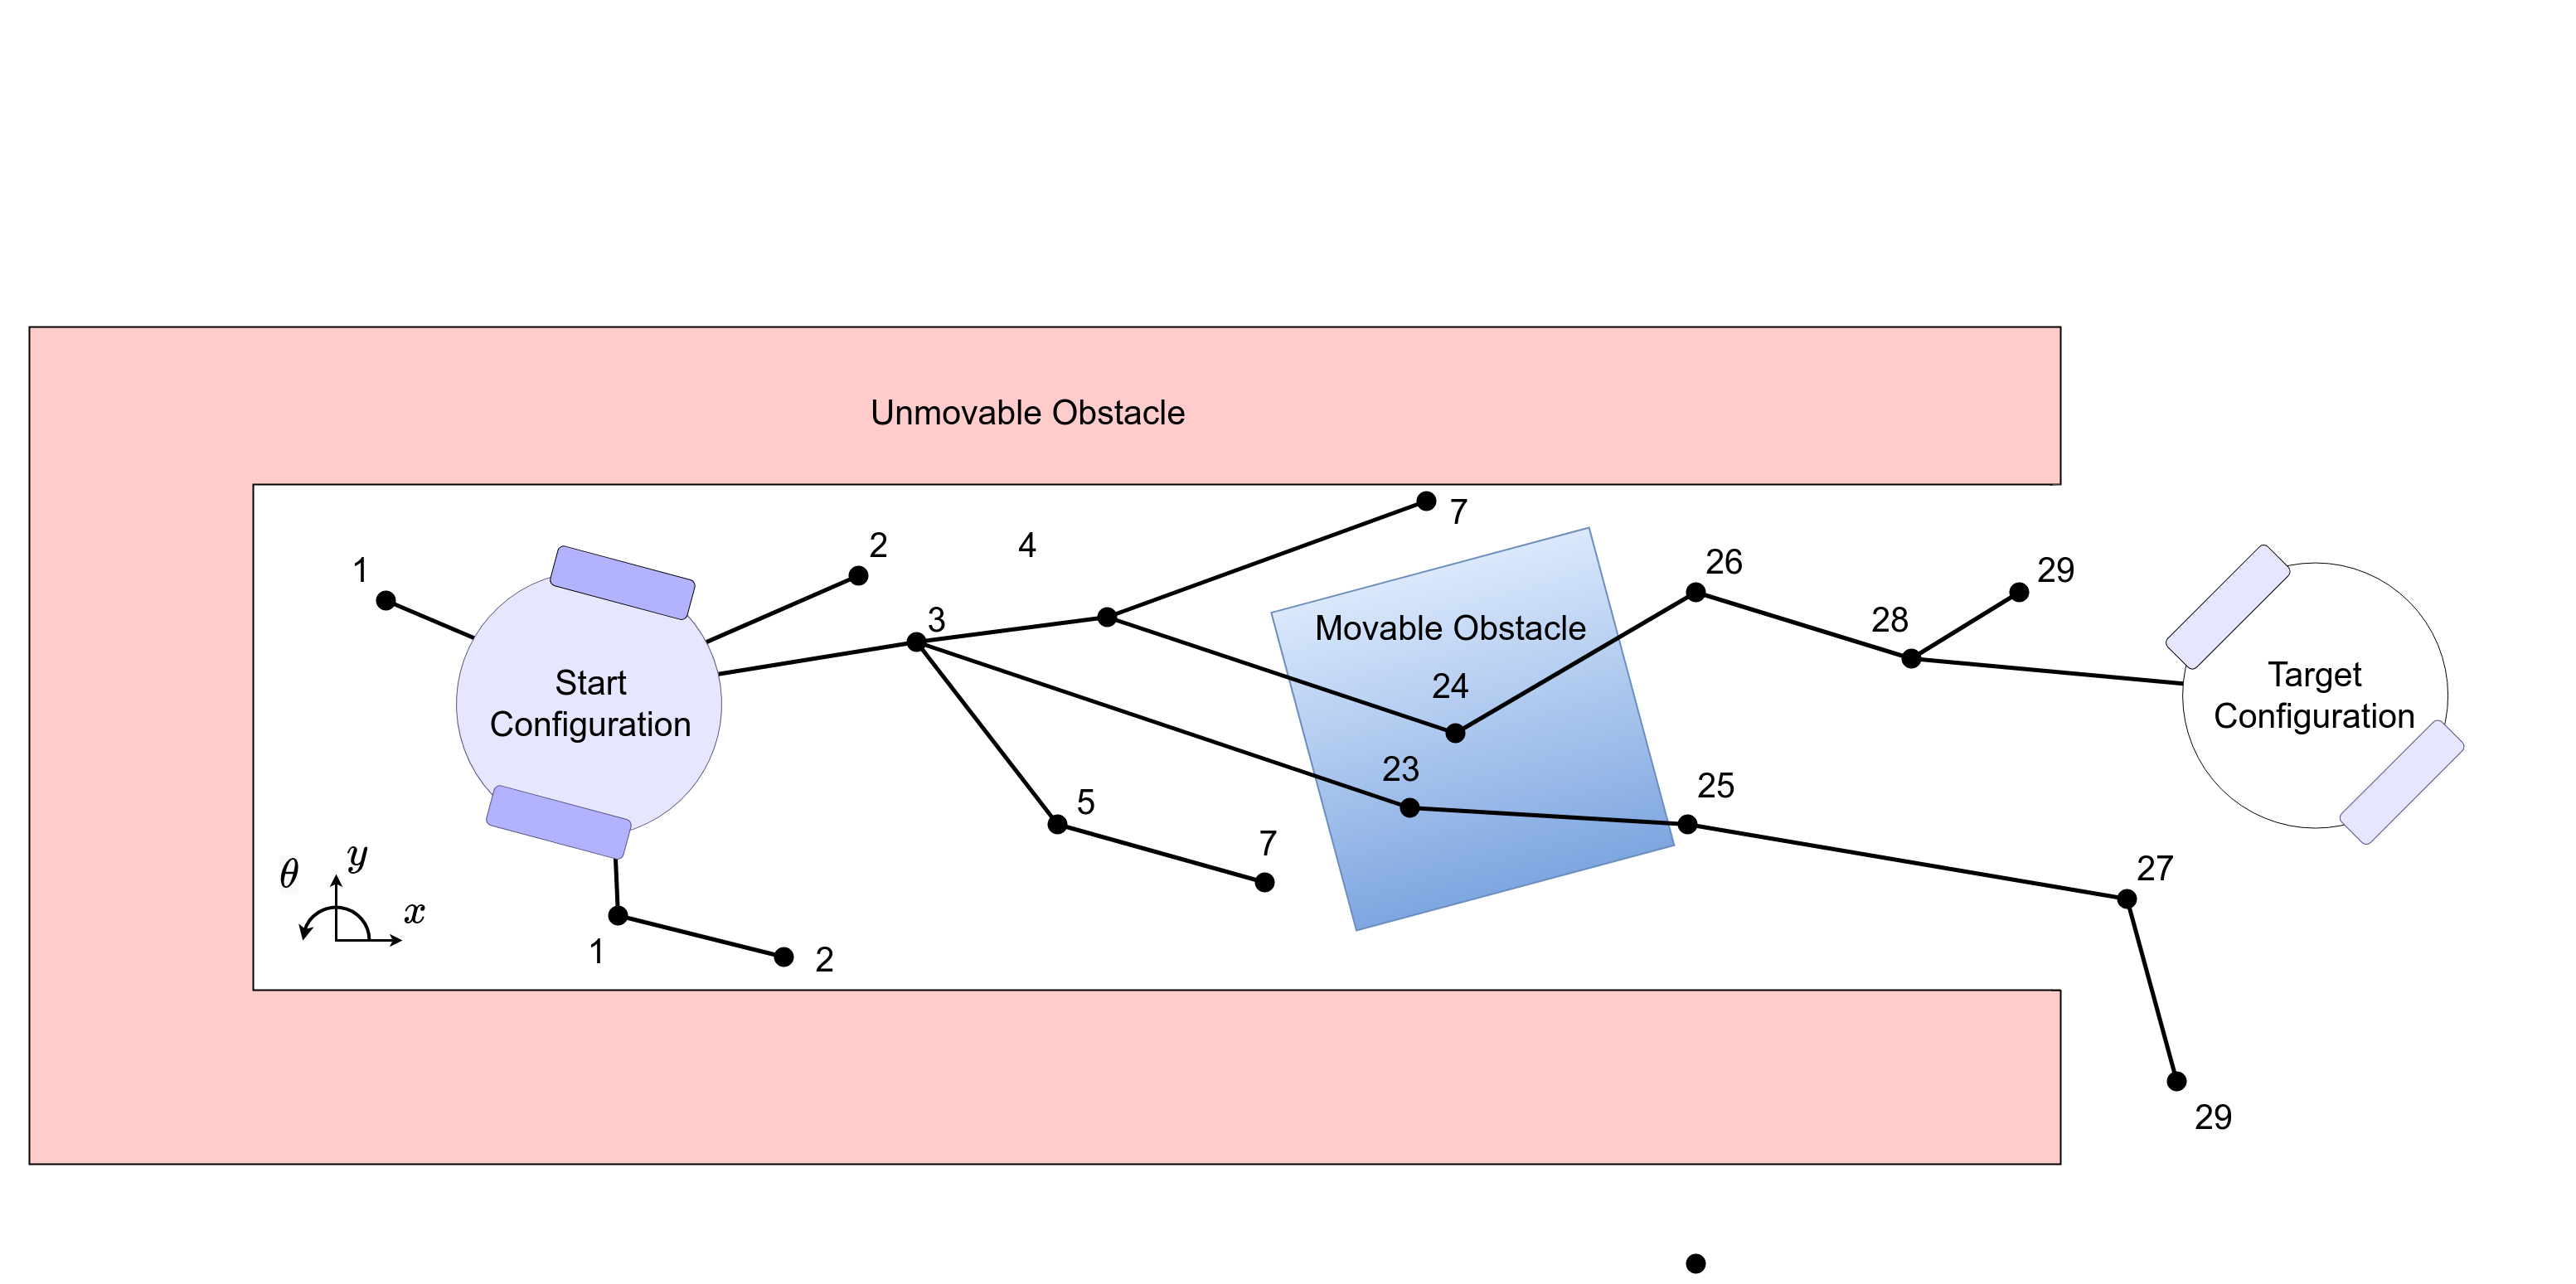
\includegraphics[width=0.9\textwidth]{figures/rrt_with_costs.png}
    \caption{Schematic view of the proposed double $\text{RRT}^*$ tree taking movable and unknown obstacles into account with cost to reach a sampled configuration displayed.}
    \label{figure: double_rrt_alg}
\end{figure}

Note that it remains hard to make predictions on the height of the cost because the object has unknown dynamics, which is why there is a fixed cost for unknown and movable obstacles, unmovable obstacles are captured by the obstacle space. \\

Algorithms \cref{pseudocode: rrt_star} displays the pseudocode for the double $\text{RRT}^*$ algorithm which takes unknown and movable obstacles into account. The following definitions are used by the $\text{RRT}^*$ algorithm. \\

$V$: A set of vertices \\
\indent $E$: A set of edges\\

The following functions are called by the \cref{pseudocode: rrt_star}.\\ 

\noindent $x_{init}$: Creates a start and target configuration. \\ $NotReachStop$: Returns true if the stopping criteria is not reached. \\ $Sample_{free}$: Creates a random sample in free space, free space includes the movable and unknown obstacles. \\ $Nearest(x, V)$: Finds the nearest vertices using euclidean distance \\ $NearestSet(x, V)$: Find a set of nearest vertices using euclidean distance \\ $Project(x, x')$: Project $x'$ toward $x$ such that it lies close enough to a vertices to be compared using a local planner \\ $CollisionCheck(x)$: returns true if $x$ is in free-space, movable obstacle or unknown obstacle \\  $CostFromInit(x, x')$: Find the total cost from $x$ to the initial vertices via $x'$, cost is determined as a sum of path length and if the path overlaps with movable of unknown objects. \\ $ConstraintsCheck(x, x')$: return true if a local planner is able to connect $x$ and $x'$ using a forward model. \\

\begin{algorithm}[H]
\caption{Proposed Double tree $\text{RRT}^*$ algorithm taking movable obstacles and constraints into account, edited $\text{RRT}^*$ pseudocode from \cite{chen_fast_2018}}
\label{pseudocode: rrt_star}
\begin{algorithmic}[1]
\State $V \leftarrow x_{init}$
\While{$NotReachStop$} 
    \State $Cost_{min} \leftarrow +\infty$
    \State $x_{rand} \leftarrow Sample_{free}$
    \State $x_{nearest} \leftarrow Nearest(x_{rand}, V)$
    \State $x_{temp} \leftarrow Project(x_{nearest}, x_{rand})$
    \If{$CollisionCheck(x_{temp}) == True$}
        \State $x_{new} = x_{temp}$
        \Else
        \State $Continue$
    \EndIf
    \State $X_{near} \leftarrow NearestSet(x_{new}, V) $
    \For{$x_{near} \in X_{near}$}
        \If{$CostFromInit(x_{new}, x_{near}) < Cost_{min}$}
            \If{$ConstraintsCheck(x_{new}, x_{near}) == True $}
            \State $Cost_{min} \leftarrow CostFromInit(x_{new}, x_{near})$
            \State $x_{minCost} \leftarrow x_{near}$
            \EndIf
        \EndIf
    \EndFor
    \If{$Cost_{min} != \infty$}
        \State $V.add(x_{new})$
        \State $E.add(x_{minCost}, x_{new})$
    \EndIf
\EndWhile
\end{algorithmic}
\end{algorithm}

\paragraph{Notation standard}
For the upcoming \cref{section: hgraph,section: knowledge_graph}, especially for the definitions of the hypothesis and knowledge graph a notation standard is used. A list of hypothesis and knowledge graph related symbols is shown in \cref{table: symbol_list_hgraph}.\\

Subscripts are used to indicate what the variable belongs to. For example, the state variable of the robot is written down as $s_{robot}$. Certain variables indicate the same object, but with different values, this is indicated by different superscripts. For example $s_{robot}^1$ and $s_{robot}^2$ are different states but both indicate the robot's state, formally $||s_{robot}^1-s_{robot}^2|| \neq 0$. $k$ indicates the time step, for example, the state of the robot at time step $k$: $s_{robot}(k)$. For convenience, the time step index is sometimes dropped. \\ 

\renewcommand{\arraystretch}{1.2}
\begin{table}[H]
    \centering
    \begin{tabular}{p{2cm} l }
        $k$ & \textrm{time step index}\\
        $s_{id}(k)$: & \textrm{State}\\
        $c_{id}(k)$: & \textrm{Configuration}\\
        $\mathcal{C}_{id}(k)$: & \textrm{configuration set}\\
        $ob_{id}(k)$: & \textrm{Object}\\
        $\mathcal{O}_{id}(k):$ & \textrm{Object set}\\
        $V^{ob}_{id}$: & \textrm{node storing set of objects}\\
        $V^{conf}_{id}$: & \textrm{node storing set of configurations}\\
        $V^{\Delta conf}_{id}$: & \textrm{node storing set of configurations and boolean lists}\\
       $d$: & \textrm{dynamical model}\\
        $\alpha$: & Success factor\\
        $\tau_{(i,j)}$: & \textrm{Transition}\\
        $G^{knowledge}$: & \textrm{knowledge graph}\\
        $G^{hypothesis}$: & \textrm{hypothesis graph}\\
        $h$: & \textrm{plan, hypothesis}\\
        $path$: & \textrm{list of configurations indicating a path, or False}
   \end{tabular}
    \caption{List of symbols used in the hypothesis- and knowledge graph, where $id$ is a unique identifier of the object}
    \label{table: symbol_list_hgraph}
\end{table}

\section{Hypothesis Graph}%
\label{sec:hgraph}
The \ac{halgorithm} is responsible for generating action sequences, called hypothesis. An hypothesis consists of a list of successive edges in the \ac{hgraph} from start to target node in the \ac{hgraph}. When all subtasks in a task are completed, the \acf{halgorithm} halts and concludes the task successfully completed. A search in the joint configuration space is avoided because an edge only operates in a single mode of dynamics, such as driving or pushing. When an object cannot directly be steered toward its target location new nodes are generated which need to be completed before the original object can be steered toward its target location. An example of when an object cannot directly be steered toward its target state is because the path is blocked by another object. A hypothesis, consisting of a list of edges that represent actions in the robot environment might succeed or fail. \Cref{tikz:flowchart_hgraph} displays a flowchart explaining how new nodes and edges are generated in the \ac{hgraph}. Successfully completed edges eventually result in completed subtasks, failed edges trigger replanning that will restart the search to a hypothesis.\bs

The \ac{halgorithm} with the \ac{hgraph} have a familiar structure compared to some recent literature~\cite{ellis_navigation_2022,wang_affordancebased_2020}. An important distinction is that the proposed method in this thesis aims to combine the 3 topics: learning object dynamics, solving \ac{NAMO} problems and nonprehensile pushing. Recent literature is able to only combine one or two topics of the three.\bs

In the upcoming section the \ac{hgraph} is defined and discussed in \cref{subsec:hgraph_definition}. The \ac{halgorithm} is then discussed and in \cref{subsec:halgorithm}, where an explanation is provided on how the \ac{halgorithm} searches for a solution in the joint configuration space. The section is concluded with an extensive example.\bs

\subsection{Definition}%
\label{subsec:hgraph_definition}%
Before defining the \ac{hgraph}, some definitions are defined on which the \ac{hgraph} depends. First, recall the \textbf{state} defined in the \cref{sec:problem_description}.\bs

An object holds the information about an object.\\Formally, a \textbf{object},  $obst_{id}(k) = \left\langle s(k), shape \right\rangle $\bs

where $shape$ is linked to a 3D representation of the object which is used to construct the configuration space.\bs

An object node represents an object in a state.\\Formally, a \textbf{objectNode}, $V^{obst}_{id} =\left\langle \textrm{status}, obst(k)\right\rangle $\\where status indicates if the node has been visited in the \ac{hgraph}. $\textrm{status} = (Initialised, Completed, Failed)$\bs

An edge describes the details of how a node transitions to another node in the \ac{hgraph}. In the robot environment, an edge represents a change of state for an object. System identification and performing an action such as pushing or driving both change the state of objects in the robot environment, but because are very different, the edges are split into 2 categories. IdentificationEdges that collect system \ac{IO} data and convert that into a system model. And actionEdges that plan and track a motion from a start to a target state. Formally:\bs

A \textbf{identificationEdge},
\todo[inline]{define identificationEdge, currently hard coded models are used in the implementation}

A \textbf{actionEdge}, $\tau_{(from, to)} = \left\langle \textrm{status}, id_{from}, id_{to}, \textrm{verb}, \textrm{controller},\textrm{dynamic model}, \textrm{path}\right\rangle$\bs

with $id_{from}$ and $id_{to}$ indicating the node id of the node in the \ac{hgraph} where the edge start from and point to respectively, $verb$ an English verb describing the action the edge represents, the controller contains the controller used for driving the robot, the dynamic model is the dynamic model used by the controller, path a list of configurations indicating the path connecting a start- to target node.\bs
\todo[inline]{Martijn: what does this mean: "the controller contains the controller..."?}

A $verb = \{\textrm{driving, pushing}\}$.\bs

Now the nodes and edges have been defined, the \ac{hgraph} can be defined.\bs

Formally, a \textbf{hypothesis graph}, $G^{hypothesis} = \left\langle V, E \right\rangle $ 
\\comprising $V = \{V^{ob}_{i}\}$, \quad $E \in \{\tau_{(i,j)}| V_i, V_j \in \{V^{ob} \}, i \neq j\}$.\bs

Most \ac{hgraph} components have now been defined. The status of an identification edge or action edge still remains undefined and requires some further explanation.\bs

\paragraph{Status, Types and Lifetime of edges}
Because system identification and tracking a path are so very different, the edges are split into two categories, identification edges and action edges. An identification edge, which is responsible for sending an input sequence to the system and recording the system output. That input/output sequence and assumptions on the system are the basis for system identification, techniques on various system identification methods are discussed in \cref{sec:sys_iden}. The goal is to create a dynamical model which is augmented with a corresponding controller is closed-loop stable.\bs

An identificationEdge, the status can be visualised in \cref{tikz:status_identification_edge}.\bs

\begin{figure}[H]
\centering
\begin{tikzpicture}[node distance = 2cm, auto, initial]
    \node [state, fill=my_dark_blue] (init_test_num) {IT\#t};
    \node [state, fill=my_light_blue, below of=init_test_num] (completed_test_num) {CT\#t};
    \node [state, accepting, fill=my_green, below of=completed_test_num] (completed) {CO};
    \node [state, accepting, fill=my_red, right of=completed_test_num, node distance=6cm] (failed) {FAIL};

 % arrows
    \draw [-stealth] ([xshift=-2cm]init_test_num.west) to node[near start,above]{\shortstack[]{select compatible\\sys. iden. method}} (init_test_num.west);
    \draw[-stealth] (init_test_num) edge[bend right] node[left]{Collect \ac{IO} data} (completed_test_num)
(completed_test_num) edge node[left]{create system model} (completed);
    \draw [-stealth] (completed_test_num) edge[bend right] node[right]{goto next start state} (init_test_num);
    \draw [-stealth] (completed_test_num) to node[]{Unable to reach next start state}  (failed.west);
    \draw [-stealth] (init_test_num) [out=0, in=90] to node[above]{Unable to reach next pos}  (failed.north);

\end{tikzpicture}
\caption{\acs{FSM} displaying the status of an identification edge}%
\label{tikz:status_identification_edge}
\end{figure}

\todo[inline]{some explainer on this status of iden edge}

The second type of edge is an actionEdge, containing a drive or push action. An actionEdge ready for execution contains all the necessary information to send input to the robot resulting in an object being steered toward it's target state. Before an edge is ready for execution it should be initialised properly, more specifically: initialised, path estimated should be performed, a system model must be initiated and path planning must be performed. Then finally the edge is ready to be executed and send input toward the robot, an \ac{FSM} of the actionEdge's status can be visualised in \cref{tikz:status_action_edge}.\bs

\begin{figure}[H]
\centering
\begin{tikzpicture}[node distance = 2cm, auto, initial]
    % \node [state, fill=lavenderIndigo] (init) {IN};
    \node [state, fill=my_purple] (init) {IN};
    \node [state, fill=my_dark_blue, below of=init] (path_exist) {PE};
    \node [state, fill=my_light_blue, below of=path_exist] (system_model) {SM};
    \node [state, fill=my_green, below of=system_model] (path_planned) {PP};
    \node [state, fill=my_yellow, below of=path_planned] (executing) {EX};
    \node [state, accepting, fill=my_orange, below of=executing] (completed) {CO};
    \node [state, accepting, fill=my_red] (failed) at ([xshift=4cm]$(system_model)!0.5!(path_planned)$) {FAIL};
    
 % arrows
    \draw [-stealth] ([xshift=-2cm]init.west) to node[near start,above]{select controller} (init.west);
    \draw[-stealth] (init) edge node[left]{graph-based path estimation} (path_exist)
      (path_exist) edge[bend right] node[left]{load in system model} (system_model)
(system_model) edge[bend right] node[left]{motion planning} (path_planned)
(path_planned) edge[bend right] node[left]{goto execution loop} (executing)
(executing) edge[bend right] node[left]{completed} (completed);

    \draw [-stealth] (init.east) [out=0, in=90] to node[xshift=0.1cm, right]{path non-existence proven}  ([yshift=-0.03cm,xshift=0.2cm]failed.north);
    \draw [-stealth] (path_exist.east) [out=0, in=90] to node[xshift=-0.6cm,yshift=0.55cm, above]{\shortstack[l]{system\\identification\\error}}  ([yshift=-0.03cm,xshift=-0.2cm]failed.north);
    \draw [-stealth] (system_model.east) [out=0, in=180] to node[xshift=0.1cm, yshift=0.3cm, above]{\shortstack[l]{motion\\planning\\error}} (failed.west);
    node[right]{motion planning error}  
    ([yshift=-0.3cm]failed.west);
    \draw [-stealth] (executing.east) [out=0, in=-90] to node[xshift=0.1cm,right]{fault detected}(failed.south);

\end{tikzpicture}
\caption{\acs{FSM} displaying the state of an action edge}%
\label{tikz:status_action_edge}
\end{figure}

% \par\smallskip\noindent
\centerline{\begin{minipage}{0.8\textwidth}
\begin{enumerate}
  \item[INITIALISED (IN)] The edge is created with a source and target node which are present in the \ac{hgraph}. A choice of controller is made.
    \item[PATH EXISTS (PE)] A graph-based search is performed to validate if the target state is reachable assuming that the system is holonomic.
    \item[SYSTEM MODEL (SM)] A dynamics system model is provided to the controller residing in the edge.
    \item[PATH PLANNED (PP)] Resulting from a sample-based planner, a path from start to target state is provided. 
    \item[EXECUTING (EX)] The edge is currently receiving observations from the robot environment and sends back robot input. 
    \item[COMPLETED (COMPL)] The edge has driven the system toward its target state and its performance has been calculated.
    \item[FAILED (FAIL)] An error occurred, yielding the edge unusable. 
\end{enumerate}
\end{minipage}}
\par\smallskip

\Cref{tikz:status_action_edge} shows that many steps must successfully be completed before the robot can start executing. The performance of an edge during execution, measured in various metrics (\cref{sec:proposed_method_metrics} is dedicated to metrics) is dependent on many aspects. Such as the choice of controller, the path estimation, the system model yielded by the identification edge and the path yielded by motion planning. Now that he \ac{hgraph} is defined, let's see how it is generated in the upcoming section.\bs

\subsection{\acl{halgorithm}}%
\label{subsec:halgorithm}
This section will provide a mathematical description of the proposed \ac{halgorithm}, the search and execution loop are discussed. The section will finalise with 4 examples. First, let's look into the math of the \ac{halgorithm}.\bs

\todo[inline]{a mathematically solid describtion of your backward search algorithm}

During a backward search, edges are added pointing toward the target node (or to nodes that point toward the target node). Trying to connect the robot node through a list of succesive directed edges to a target node. If such a path has been found in the \ac{hgraph}, a hypothesis has been found and the robot can start executing edges.

A flowchart of the \ac{halgorithm} is presented in \cref{tikz:flowchart_hgraph}. Compared to the mathematical description of the \ac{halgorithm} the flowchart provides more detail, including an eleborate description for every block in the flowchart (see \cref{table:explainer_hgraph_figures_nodes}). The flowchart includes path estimation, planning and the behavior when failure occures. A connection point to the \ac{kgraph} and robot environment are included. The blocks in the flowchart indicate which action they take and where, such as the configuration space, the \ac{kgraph} or the \ac{hgraph}. With the flowchart is straigtforward to see how the \ac{halgorithm} connects to the status of edges, with the mathematical description of the \ac{halgorithm} that is harder so see. Compared to the flowchart the mathematical description is a abstacted version, leaving many details out that are related to the robot in this thesis. An abstracted mathematical description is simpler and encompasses a broader field of robots. So could the mathematical description also be applied to another robot such as a movable robot with robot arm and gripper. The flowchart encompasses to many details to be applied after such an change in robot hardware. 

\input{mainmatter/hypothesis_graph/hgraph_tikz_figure}

\begin{table}[H]
\centering
\rowcolors{2}{white}{myLightColor}
\begin{tabular}[t]{>{\raggedright}p{3.5cm}>{\raggedright\arraybackslash}p{10.5cm}}
  \textbf{Node name} & \textbf{Description of actions taken}\\\toprule
  Task Finished & log all metrics for the \ac{hgraph}, then deconstruct \ac{hgraph}.\\
  Create Start and\newline Target Nodes & Generate a robot node and the start and target nodes for every subtask in the task.\\
Update Current Subtask & Select an unfinished subtask or update current subtask. Use the backward search technique. The \textit{current\_start\_node} and \textit{current\_target\_node} are updated. When all subtask have been addressed, conclude task is finished. \\
Estimate Path\newline Existence & Check if a path exists between \textit{current\_start\_node} and \textit{current\_target\_node} whilst assuming that the object is holonomic.\\
Add Node to\newline Drive to Object & Add a node before the \textit{current\_target\_node}.\\
Unfeasible Node & Update node's status to unfeasible because is can not be completed, log failed Edge.\\
Knowledge Available& Query the \ac{kgraph} for action suggestion to connect \textit{current\_target\_node} to \textit{current\_target\_node}\\
Knowledge Usable& Check if a suggested action is not on the blacklist.\\
Object Movable & Check if object is classified as movable\\
Robot Close to Object& Check if the object is inside directly reachable free space of the robot \\
Generate Random\newline Action& Randomly sample a controller with a compatible system identification method that is not on the blacklist. \\
All Possible Actions Failed & Every possible action is on the blacklist for the \textit{current\_target\_node}, update \textit{current\_target\_node} status to failed.\\
Add Drive System Identification Edge & Adds identification edge between a newly generated node and the drive action edge source node. \\
Model Available& Checks if the drive action edge contains a system model. \\
Action Type& Checks the action type. \\
Model Available& Checkif the push action edge containts a system model. \\
Add Push System\newline Identification Edge& Adds identification edge compatible with push action edge. \\
Motion Planning& Search a path for the \textit{current\_edge}, detect blocking objects. \\
Add Node to Free Path & Search closeby pose for object to free path. Create node to push object toward that pose. \\
Manipulation Planning & Search a path for the \textit{current\_edge}, detect blocking objects.\\
Add Node to Drive\newline to Push Pose& Create node to drive toward push pose, add before action edge. \\
Robot Close to\newline Push Pose & Check if the robot is overlapping with the best push position. \\
Path to Target& Is there a path from robot to target node in the \ac{hgraph}, then set first edge to \textit{current\_edge} otherwise update subtask.\\
First Action Planned&  Check if motion/manipulation planning was performed. \\
Execute& Execute the \textit{current\_edge}, update \ac{hgraph} after completion, log failed hypothesis if a fault is detected. \\
Subtask Succesfully\newline Completed& Log hypothesis metrics. \\
Target Node Reached& Check if the target node is reached.\\
\end{tabular}
\caption{Eleborate information on actions taken by blocks in \cref{tikz:flowchart_hgraph}.}%
\label{table:explainer_hgraph_figures_nodes}
\end{table}

When all tuning parameters are set, the \ac{hgraph} is initialized and a task is provided, there is only a single access point toward the \ac{hgraph}. A function \textit{respond(observation)} that provides the \ac{halgorithm} with sensor measurements of the environment with the argument \textit{observation}. The function \textit{respond($\cdot$)} returns control in put for the robot. In this theses, the sensor measurements are the configuration of objects in the environment. Recall that the perfect-sensor assumption, assumption~\ref{assumption:perfect_object_sensor} that makes access to the exact configuration of every object possible.\bs


\paragraph{The Blacklist}%
Undesirable behavior is to generate an edge that fails, only to regenerate and fail again. This infinite behavior is prevented by the blacklist. When the \ac{halgorithm} connects two nodes with an action edge, the possible parameterizations (controller and system model) are filtered. Thus any parameterisation that is on the blacklist for this specific node (to which the action edge would point toward) cannot be created again for the lifetime of the \ac{hgraph}. An example where the blacklist can be seen in action is \cref{fig:failure_in_hgraph}.\bs

\todo[inline]{math def for blacklist on the nodes}


\subsection{The Search and the Execution loop}%
\label{subsec:two_loops}
In \cref{tikz:flowchart_hgraph} two main loops can be identified, see \Cref{fig:two_loops_identified}. These loops are the search loop, and the execution loop.\bs

\begin{figure}[H]
    \centering
    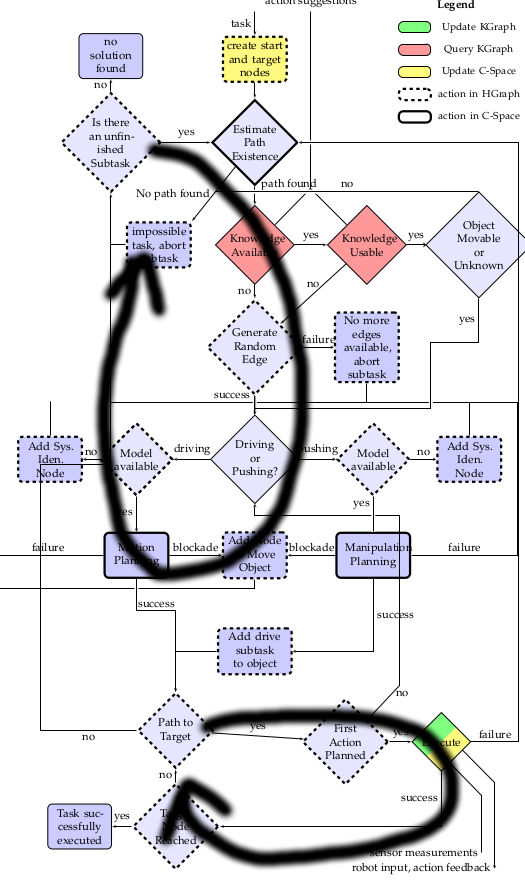
\includegraphics[width=7cm]{figures/two_loops_identified}
    \caption{The search (above) and execution (below) loop.}%
    \label{fig:two_loops_identified}
\end{figure}

Whilst the \ac{halgorithm} resides in the search loop, hypotheses are formed. Forming a hypothesis generates nodes, edges, and progressing their status as described in \cref{tikz:status_identification_edge,tikz:status_action_edge}. In the execution loop \textit{an edge is being executed}, a phrase to describe that the controller residing in an edge is sending control input toward the robot. The \ac{halgorithm} operates synchronously, thus at any point in time, the \ac{halgorithm} resides in a single block within \cref{tikz:flowchart_hgraph}. The result is that the robots cannot operate whilst the \ac{halgorithm} resides in the search loop, and during execution, no hypothesis can be formed or updated. Assumption~\ref{assumption:closed_world} guarantees that the robot environment does not change causing existing hypotheses to be outdated.\bs

\subsection{Examples}%
\label{subsec:hgraph_example}

Before displaying example \ac{hgraph}'s a legend is now presented.\bs

\begin{figure}[H]
    \centering
    \begin{subfigure}{0.2\textwidth}
    \centering
    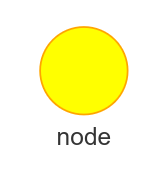
\includegraphics[width=0.7\textwidth]{figures/connecting_nodes/legend/node}
    \caption{Regular node created by the \ac{halgorithm}.\newline}%
    \end{subfigure}
    \begin{subfigure}{0.2\textwidth}
    \centering
    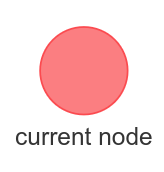
\includegraphics[width=0.7\textwidth]{figures/connecting_nodes/legend/current_node}
    \caption{Current node indicates that it's outgoing edge is now or is next to be executed.}%
    \end{subfigure}
    \begin{subfigure}{0.2\textwidth}
    \centering
    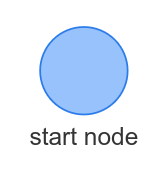
\includegraphics[width=0.7\textwidth]{figures/connecting_nodes/legend/starting_node}
    \caption{Starting node, one is generated at for every subtask.}%
    \end{subfigure}
    \begin{subfigure}{0.2\textwidth}
    \centering
    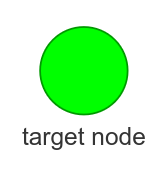
\includegraphics[width=0.7\textwidth]{figures/connecting_nodes/legend/target_node}
    \caption{Target node, one is generated for every subtask.\newline}%
    \end{subfigure}

    \begin{subfigure}{0.33\textwidth}
    \centering
    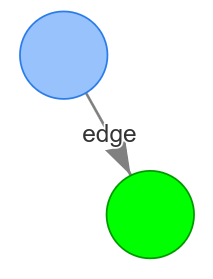
\includegraphics[width=0.7\textwidth]{figures/connecting_nodes/legend/edge}
    \caption{Edge with status IN, PE, SM, PP or EX.}%
    \end{subfigure}
    \begin{subfigure}{0.33\textwidth}
    \centering
    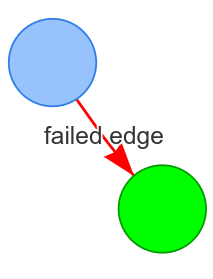
\includegraphics[width=0.7\textwidth]{figures/connecting_nodes/legend/failed_edge}
    \caption{Edge with status FAILED (FAIL)}%
    \end{subfigure}
    \begin{subfigure}{0.33\textwidth}
    \centering
    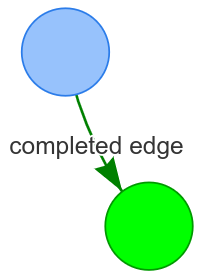
\includegraphics[width=0.7\textwidth]{figures/connecting_nodes/legend/completed_edge}
    \caption{Edge with status COMPLETED (CO)}%
    \end{subfigure}
    \caption{Legend for \ac{hgraph}'s nodes an edges}%
    \label{fig:hgraph_legend}
\end{figure}

\paragraph{Driving and Pushing} Four examples are presented, starting with a driving task in \cref{fig:robot_drive_hgraph}, then a pushing task in \cref{fig:robot_push_hgraph}.\bs

\begin{figure}[H]
    \centering
    \begin{subfigure}{.3\textwidth}
    \centering
    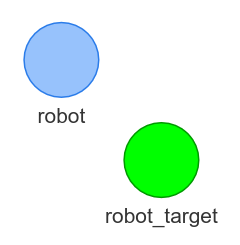
\includegraphics[width=0.7\textwidth]{figures/connecting_nodes/robot_to_target/robot_to_target}
    \end{subfigure}
    \begin{subfigure}{.3\textwidth}
    \centering
    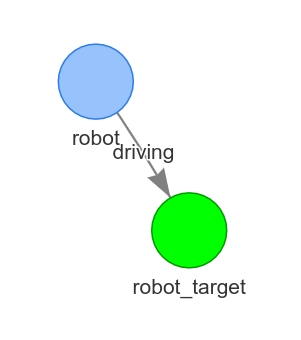
\includegraphics[width=0.9\textwidth]{figures/connecting_nodes/robot_to_target/robot_drive_target}
    \end{subfigure}
    \begin{subfigure}{.3\textwidth}
    \centering
    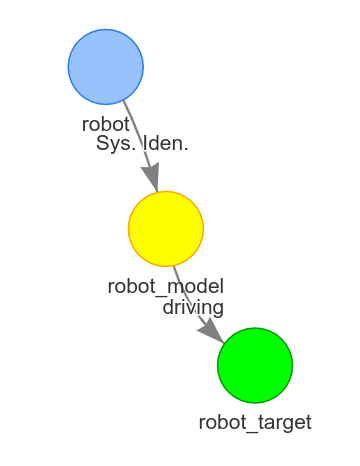
\includegraphics[width=\textwidth]{figures/connecting_nodes/robot_to_target/robot_iden_drive_target}
    \end{subfigure}
    \caption{\ac{hgraph} generated by the \ac{halgorithm} to drive the robot to a target configuration}%
    \label{fig:robot_drive_hgraph}
\end{figure}

The robot does not have a system model of itself, thus first system identification must be performed before it can drive to the specified target configuration. The \ac{kgraph} that will be discussed in \cref{subsec:kgraph_definition} can suggest an action that includes a system model. In that case, system identification is not needed. The following figure displays succesfully executing the hypothesis found in \cref{fig:robot_drive_hgraph}.\bs

\begin{figure}[H]
    \centering
    \begin{subfigure}{.3\textwidth}
    \centering
    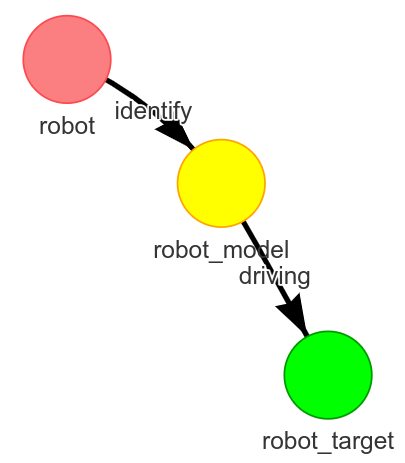
\includegraphics[width=0.8\textwidth]{figures/connecting_nodes/robot_to_target/execute_robot_to_target_1}
    \end{subfigure}
    \begin{subfigure}{.3\textwidth}
    \centering
    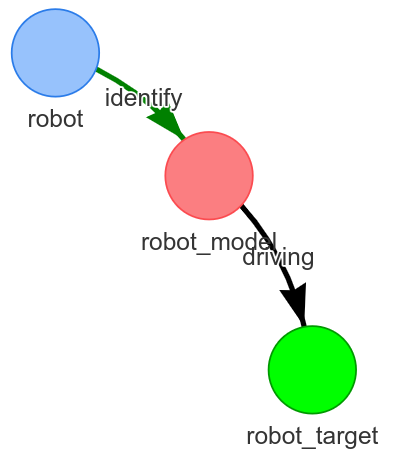
\includegraphics[width=0.8\textwidth]{figures/connecting_nodes/robot_to_target/execute_robot_to_target_2}
    \end{subfigure}
    \begin{subfigure}{.3\textwidth}
    \centering
    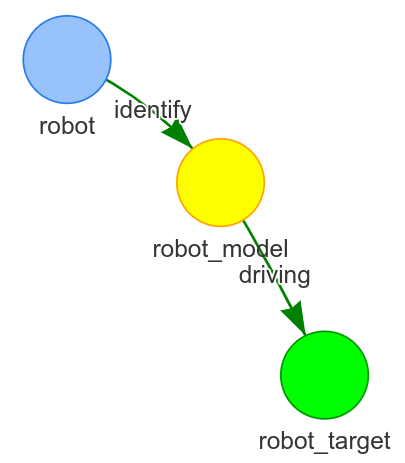
\includegraphics[width=0.8\textwidth]{figures/connecting_nodes/robot_to_target/execute_robot_to_target_3}
    \end{subfigure}
    \caption{Executing the hypothesis found in \cref{fig:robot_drive_hgraph}.}
    \label{fig:execute_robot_to_target}
\end{figure}

Upcoming figure will display the hypothesis generated to push an object to a target position. Both generating a hypothesis and executing the hypothesis are intertwined, this is because certain information should first be collected from the environment before the full hypothesis can be generated. An example is the \textit{best\_push\_position} that can be found in \cref{subfig:robot_push_7,subfig:robot_push_8,subfig:robot_push_9}. The \textit{best\_push\_position} can be found after manipulation planning for the pushing edge is completed. For motion planning a system model is required, thus the corresponding system identification edge should be completed before manipulation planning can start, and than the \textit{best\_push\_position} can be determined.\bs

\begin{figure}[H]
    \centering
    \begin{subfigure}{.3\textwidth}
    \centering
    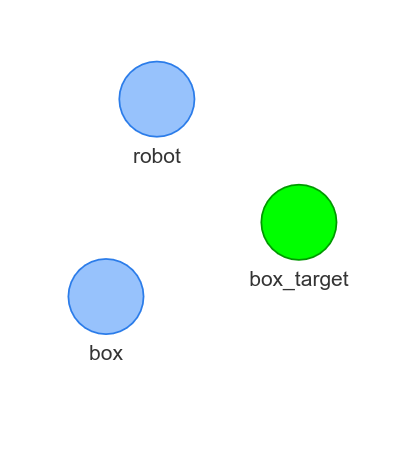
\includegraphics[width=0.8\textwidth]{figures/connecting_nodes/robot_push/robot_push_1}
    \caption{}
    \end{subfigure}
    \begin{subfigure}{.3\textwidth}
    \centering
    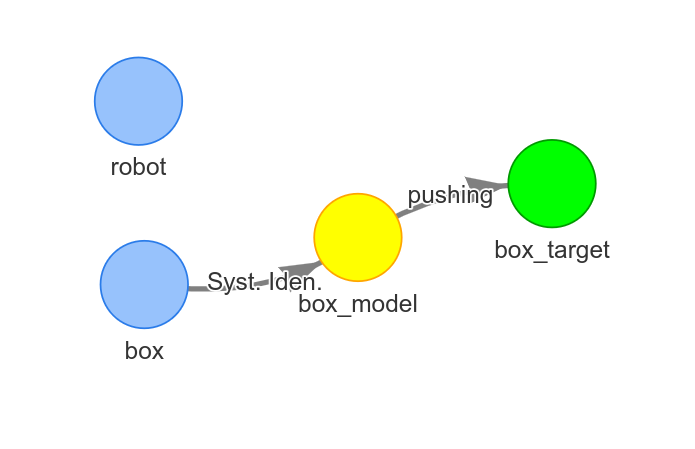
\includegraphics[width=1.1\textwidth]{figures/connecting_nodes/robot_push/robot_push_2}
    \caption{}\label{subfig:robot_push_2}
    \end{subfigure}
    \begin{subfigure}{.3\textwidth}
    \centering
    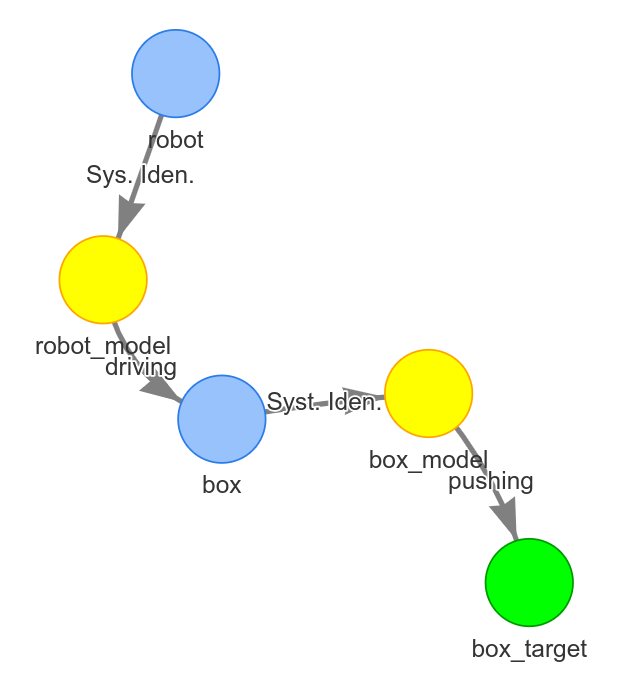
\includegraphics[width=1\textwidth]{figures/connecting_nodes/robot_push/robot_push_3}
    \caption{}\label{subfig:robot_push_3}
    \end{subfigure}

    \begin{subfigure}{.3\textwidth}
    \centering
    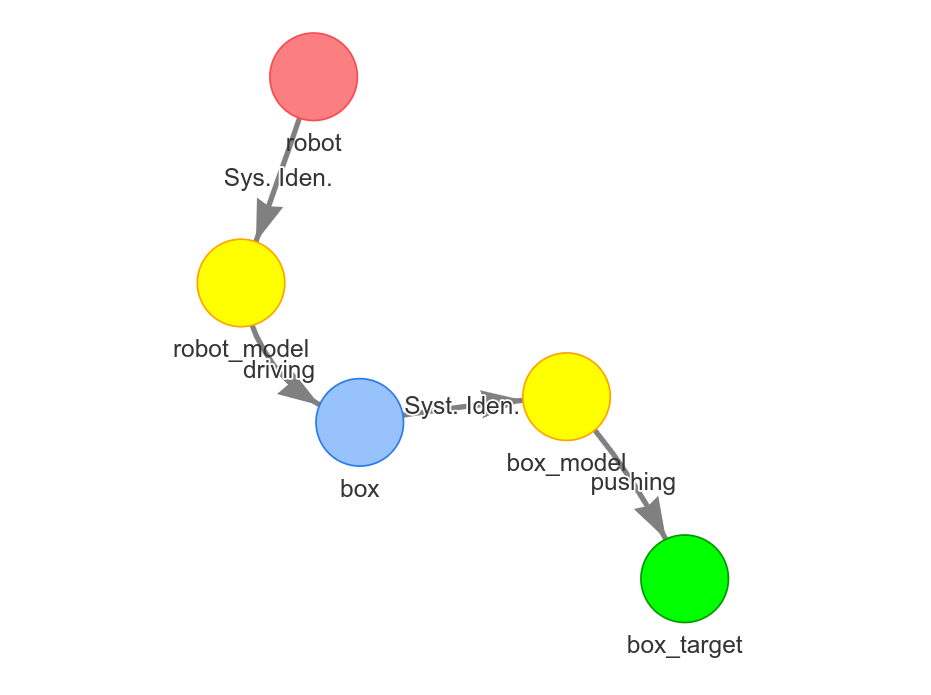
\includegraphics[width=1\textwidth]{figures/connecting_nodes/robot_push/robot_push_4}
    \caption{}\label{subfig:robot_push_4}
    \end{subfigure}
    \begin{subfigure}{.3\textwidth}
    \centering
    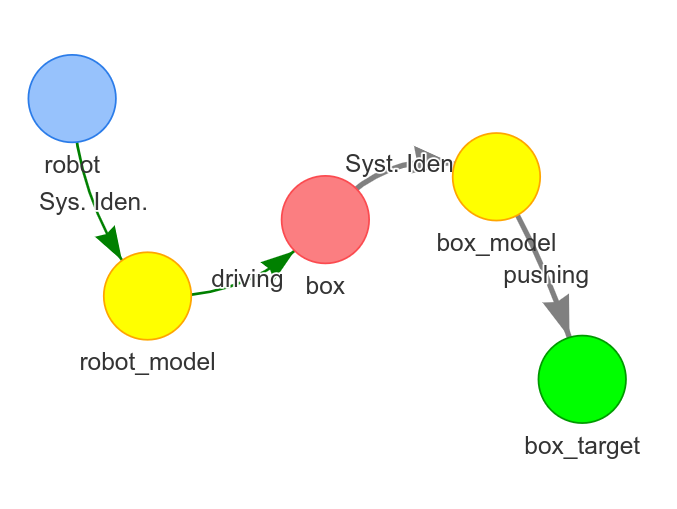
\includegraphics[width=1.05\textwidth]{figures/connecting_nodes/robot_push/robot_push_5}
    \caption{}\label{subfig:robot_push_5}
    \end{subfigure}
    \begin{subfigure}{.3\textwidth}
    \centering
    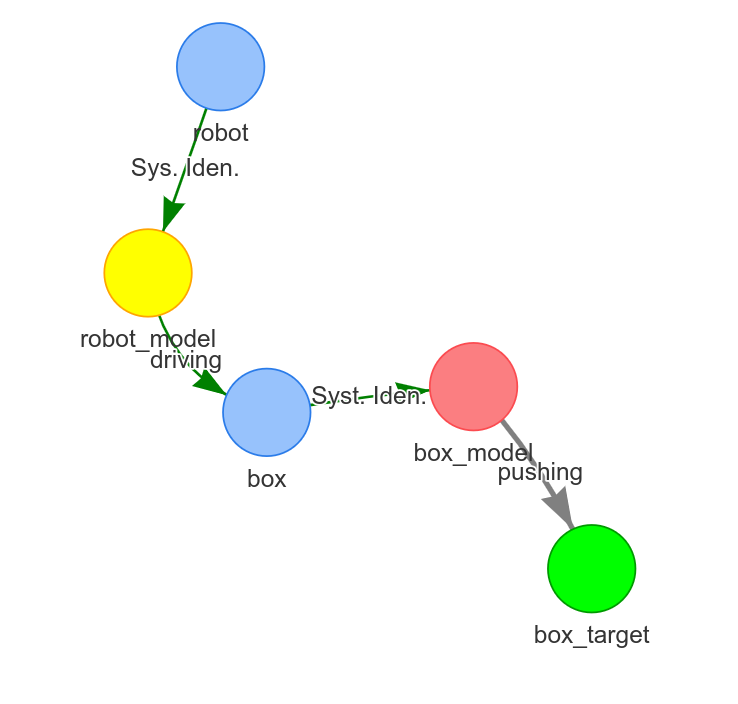
\includegraphics[width=1.05\textwidth]{figures/connecting_nodes/robot_push/robot_push_6}
    \caption{}\label{subfig:robot_push_6}
    \end{subfigure}

    \begin{subfigure}{.3\textwidth}
    \centering
    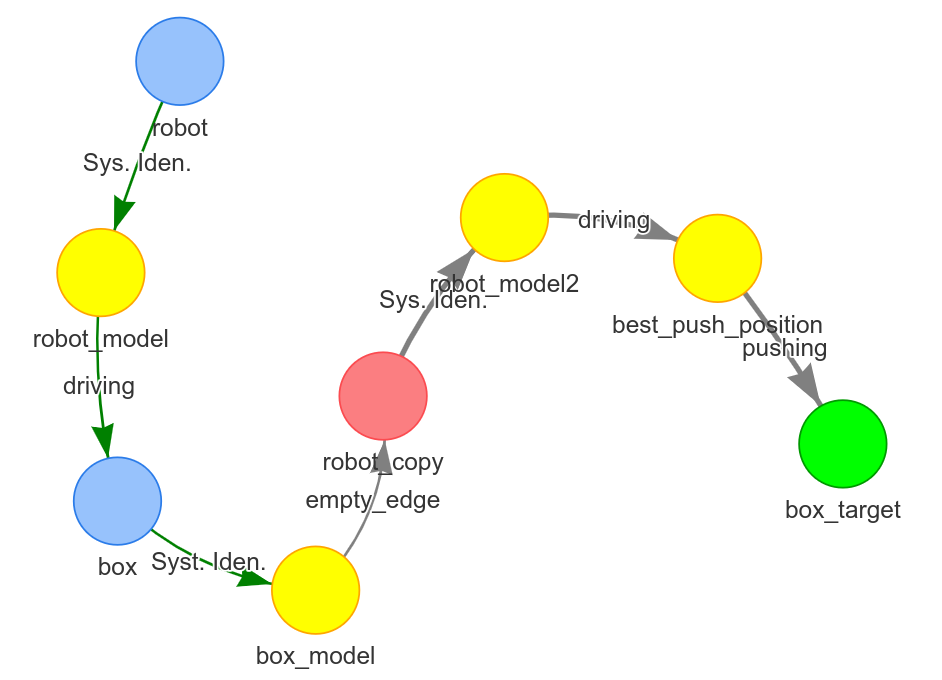
\includegraphics[width=1\textwidth]{figures/connecting_nodes/robot_push/robot_push_7}
    \caption{}\label{subfig:robot_push_7}
    \end{subfigure}
    \begin{subfigure}{.3\textwidth}
    \centering
    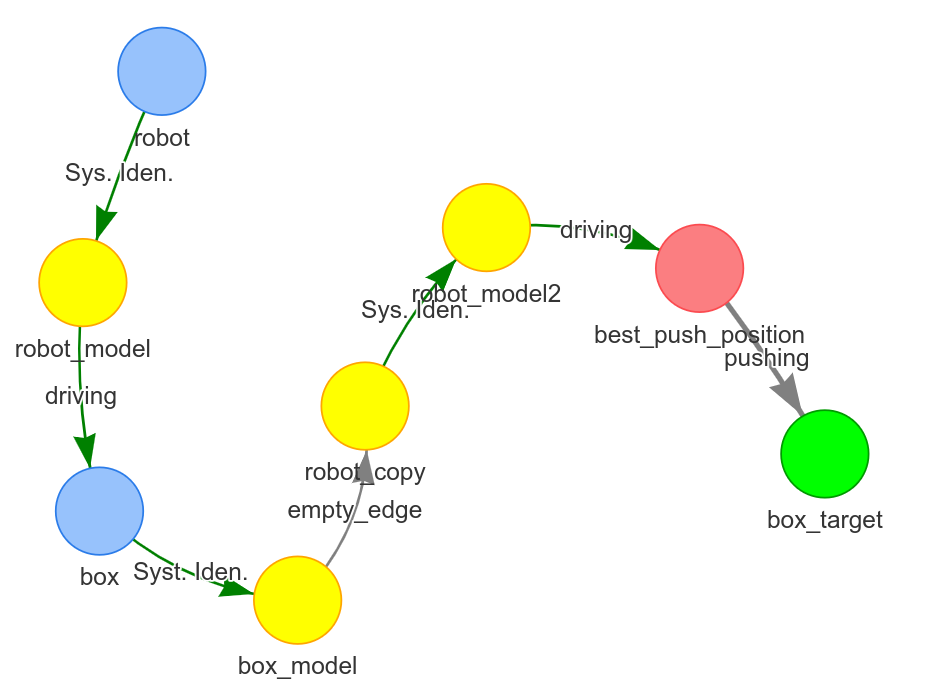
\includegraphics[width=1.05\textwidth]{figures/connecting_nodes/robot_push/robot_push_8}
    \caption{}\label{subfig:robot_push_8}
    \end{subfigure}
    \begin{subfigure}{.3\textwidth}
    \centering
    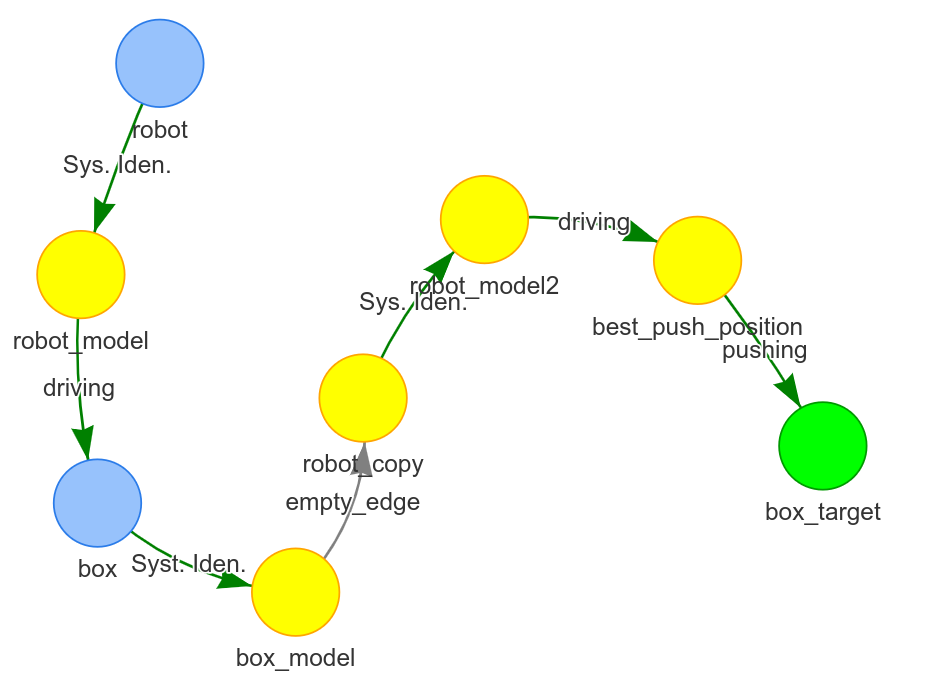
\includegraphics[width=1.05\textwidth]{figures/connecting_nodes/robot_push/robot_push_9}
    \caption{}\label{subfig:robot_push_9}
    \end{subfigure}
    \caption{\ac{hgraph} for pushing the green box to the target configuration}%
    \label{fig:robot_push_hgraph}
\end{figure}
Especially in \cref{subfig:robot_push_2,subfig:robot_push_3} the backward search is clearly visible, the \ac{halgorithm} searches from target node to the robot node. \Cref{fig:robot_push_hgraph} is extensive because every nessecary steps is included whilst some could be skipped. First, identifying a system model for robot driving twice, if the system model created in edge Sys. Iden. pointing toward node robot\_model is reused, then the edge Sys. Iden. pointing toward robot\_model\_1 would be unnecessary. Second, if system models would already be availeble for driving and pushing, no single system identification edge would be required. A \textit{empty\_edge} can be seen in \cref{subfig:robot_push_7,subfig:robot_push_8,subfig:robot_push_9}, the empty\_edge serves to connect a node to another node (box\_model to robot\_copy in \cref{fig:robot_push_hgraph}). The empty\_edge can be traversed without execution, holds no controller, system model or status.\bs

\paragraph{Encountering a Blocked Path}%
During propagation of an action edge's status, motion or manipulation planning occurs. If an object is blocking the path, planning will detect it and the \ac{halgorithm} tries to free the path. In the next example the \ac{halgorithm} detects a blocking object and frees the path by pushing the blocking object to a new configuration, and can be visulised in \cref{fig:blocking_obj_hgraph}.\bs

\begin{figure}[H]
    \centering
    \begin{subfigure}{.3\textwidth}
    \centering
    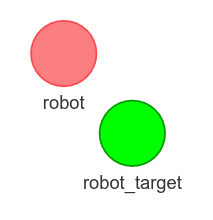
\includegraphics[width=0.5\textwidth]{figures/connecting_nodes/blocking_obj/blocking_obj_1}
    \caption{}
    \end{subfigure}
    \begin{subfigure}{.3\textwidth}
    \centering
    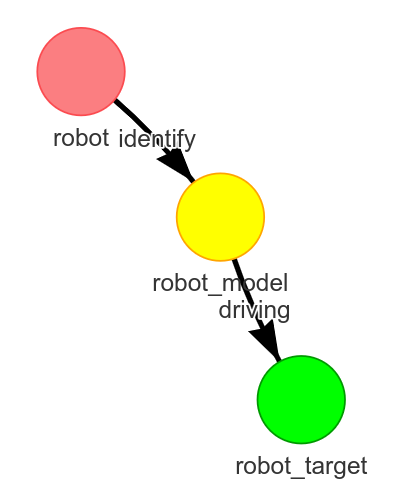
\includegraphics[width=\textwidth]{figures/connecting_nodes/blocking_obj/blocking_obj_2}
    \caption{}\label{subfig:blocking_obj_2}
    \end{subfigure}
    \begin{subfigure}{.3\textwidth}
    \centering
    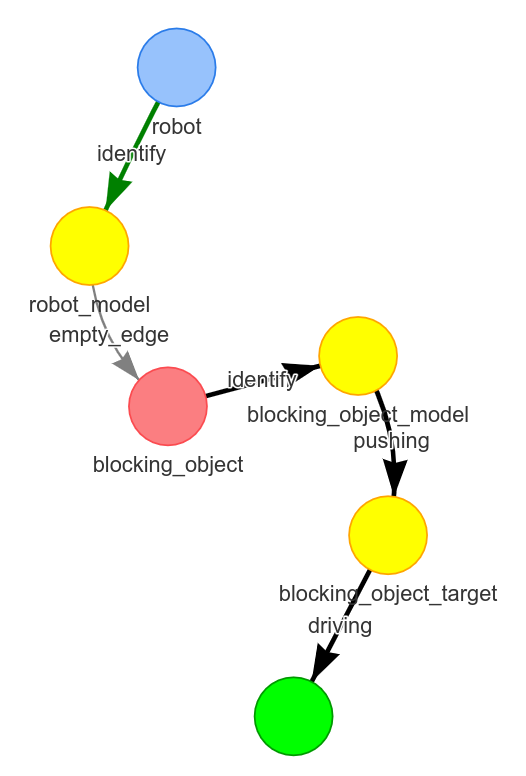
\includegraphics[width=\textwidth]{figures/connecting_nodes/blocking_obj/blocking_obj_3}
    \caption{}\label{subfig:blocking_obj_3}
    \end{subfigure}

    \begin{subfigure}{.3\textwidth}
    \centering
    \includegraphics[width=1.3\textwidth]{figures/connecting_nodes/blocking_obj/blocking_obj_4}
    \caption{}\label{subfig:blocking_obj_4}
    \end{subfigure}
    \begin{subfigure}{.3\textwidth}
    \centering
    \includegraphics[width=\textwidth]{figures/connecting_nodes/blocking_obj/blocking_obj_5}
    \caption{}\label{subfig:blocking_obj_5}
    \end{subfigure}
    \begin{subfigure}{.3\textwidth}
    \centering
    \includegraphics[width=\textwidth]{figures/connecting_nodes/blocking_obj/blocking_obj_6}
    \caption{}\label{subfig:blocking_obj_6}
    \end{subfigure}
    \caption{\ac{hgraph} for driving to target configuration and encountering a blocked path}%
    \label{fig:blocking_obj_hgraph}
\end{figure}

\paragraph{Encountering Failure}%
In the last example, the first hypothesis fails to complete and the \ac{halgorithm} tries to generate a new hypothesis that also fails to complete. Several faults and failures are modelled, the \ac{halgorithm} response to faults and failure is the same. If during the propagation of an edge's status any kind of failure arises, the failed edge and corresponding edges are marked as failed. Equally during execution, if a fault is detected, the execution halts and the edge and corresponding edges are marked as \quotes{failed}, the procedure can be seen in \cref{fig:failure_in_hgraph}.\bs

\begin{figure}[H]
    \centering
    \begin{subfigure}{.3\textwidth}
    \centering
    \includegraphics[width=0.8\textwidth]{figures/connecting_nodes/failure/fail_1}
    \end{subfigure}
    \begin{subfigure}{.3\textwidth}
    \centering
    \includegraphics[width=1.1\textwidth]{figures/connecting_nodes/failure/fail_2}
    \end{subfigure}
    \begin{subfigure}{.3\textwidth}
    \centering
    \includegraphics[width=1\textwidth]{figures/connecting_nodes/failure/fail_3}
    \end{subfigure}

    \begin{subfigure}{.3\textwidth}
    \centering
    \includegraphics[width=1\textwidth]{figures/connecting_nodes/failure/fail_4}
    \end{subfigure}
    \begin{subfigure}{.3\textwidth}
    \centering
    \includegraphics[width=1\textwidth]{figures/connecting_nodes/failure/fail_5}
    \end{subfigure}
    \begin{subfigure}{.3\textwidth}
    \centering
    \includegraphics[width=1\textwidth]{figures/connecting_nodes/failure/fail_6}
    \end{subfigure}

    \begin{subfigure}{.3\textwidth}
    \centering
    \includegraphics[width=1\textwidth]{figures/connecting_nodes/failure/fail_7}
    \end{subfigure}
    \hfill
    \caption{Executing two hypothesis, both failing to complete because a fault of failure emerged.}%
    \label{fig:failure_in_hgraph}
\end{figure}

In \cref{fig:failure_in_hgraph} only two parameterisations of drive controller and system model were available. Thus after two failed hypothesis the \ac{halgorithm} concludes it cannot complete this task.\bs


What by now hopefully became clear to the reader is that the \ac{hgraph} autonomously searches for hypotheses to solve the task, one subtask at a time. The \ac{hgraph} switches between the search and execution loop. Switching from the search loop toward the execution loop when a hypothesis is found, and switching back when a hypothesis is completed or an action failed to complete.\bs

The limited number of possible edges (every combination of a system identification method with a compatible control method) guarantees that the robot tries to connect 2 nodes, but concludes that it cannot reach a node if all possible edges have failed. Eventually running out of nodes to connect and conclude that a subtask cannot be completed.\bs

In the next section, the edges that are executed will be reviewed and stored in a knowledge base. The knowledge base will suggest edges when faced with similar nodes to connect.
\


\section{Knowledge Graph}%
\label{sec:kgraph}
The \ac{hgraph}, discussed in the previous section, spans a lifetime over a single task. In the \ac{hgraph} only the object class is stored for the lifetime of the \ac{hgraph}. When a task is completed, the \ac{hgraph} is deconstructed and learned objects classes are lost. The \ac{kgraph}'s responsibility is to store objects classes for future tasks, and to make an ordering in the edge parameterizations where a edge parameterization comprises of a controller and system model. Estimating which parameterization would be the best candidate is an entire field of research. In this thesis the ordering is made by collecting action feedback on executed action edges and summarizing that feedback in a single metric, the \textit{success factor}. This metric combines two metrics the \acl{PE} and the success-fail ratio of an edge parameterization.\bs

The name \quotes{\acl{kgraph}} originates from the environmental knowledge it contains and its graph structure. Both the \ac{hgraph} and \ac{kgraph} are newly proposed frameworks built from the ground up, with only inspiration from an already existing technique, a backward search. The \ac{kgraph} is in an early stage of development and does therefore not (yet) adhere to any standard that apply to knowledge bases, such as first order-logic~\cite{barwise_introduction_1977,rensink_representing_2004}, relational databases~\cite{atzeni_relational_1993} or more practical, a language such as prologe~\cite{wielemaker_swiprolog_2012}.\bs

\subsection{Definition}
\label{subsec:kgraph_definition}


\todo[inline]{this section}

\subsection{Edge Metrics}
\label{subsec:edge_metrics}
\subsection{Example}
\label{subsec:kgraph_example}



\newpage

\begin{figure}[H] \centering
  \begin{tikzpicture}[node distance = 4.5cm, line width=1pt]
    % Nodes
    \node [block, fill=green!50] (first) {Update existing edge with new feedback};
    
    % legend 
    \node[text width=2.8cm, yshift=1cm, right of=first, text centered, rounded corners, minimum height=1em, label={[name=lab, yshift=0.4cm, left]\textbf{Legend}}, node distance=7cm] (legend1) {\small Update KGraph};
    \node[rectangle, draw, left of=legend1, fill=green!50, rounded corners, minimum height=1em, minimum width=1cm, node distance=2cm] (legend1color) {};
    \node[text width=2.8cm, below of=legend1, text centered, minimum height=1em, node distance=0.7cm] (legend2) {\small Query KGraph};
    \node[rectangle, draw, left of=legend2, fill=red!40, rounded corners, minimum height=1em, minimum width=1cm, node distance=2cm] (legend2color) {};
   
    
    % nodes, first row 
    \node [decision, below of=first, node distance=4.5cm, fill=red!40, text width=7.0em] (has_controller) {Does this parameterization exist in one of the center node's outgiong edges?};
    \node [block, left of=has_controller, fill=green!50] (new_transition) {Generate new edge with feedback edge with feedback existing node};
    
    % nodes, second row 
    \node [decision, fill=red!40, below of=has_controller, node distance=6cm, text width=6.0em] (obj_exist) {Does this object exist in a center node in the \ac{kgraph}?};

  \node [decision, fill=red!40, right of=obj_exist, node distance=4.5cm, text width=6.0em] (obj_exist2) {Does this object exist in a center node in the \ac{kgraph}?};
    \node [block, yshift=-3cm, above= of obj_exist2, node distance=-1.8cm] (send_feedback) {Send ordered list with controllers and models};
    
    \node [block, fill=green!50, left of=obj_exist] (new_object) {Generate new center node, side node and an edge with feedback};
    \node [block, right of=obj_exist2, node distance=3.8cm] (no_obj) {send empty list};
   
    % Edges
    \draw[stealth-] (obj_exist) -- node[left, at end]{action feedback} +(0,-3.5cm);
    \draw[-stealth] (obj_exist.west) -- node[above]{no} (new_object.east);
    \draw[-stealth] (obj_exist.north) -- node[left]{yes} (has_controller.south);
    \draw[-stealth] (has_controller.north) -- node[left]{yes} (first.south);
    \draw[-stealth] (has_controller.west) -- node[above]{no} (new_transition.east);
    
    \draw[-stealth] (obj_exist2.east) -- node[above]{no} (no_obj.west);
    \draw[-] (no_obj.east) -- +(0.7cm, 0);
    \draw[stealth-] (obj_exist2) -- node[left, at end]{action suggestion?} +(0,-3.5cm);
    \draw[-stealth] (obj_exist2.north) -- node[left]{yes} (send_feedback.south);
    \draw[-stealth] (send_feedback.east) -| node[at end, left]{action suggestion} +(4.5cm, -8.4cm);
\end{tikzpicture}
\caption{Flowchart displaying the knowledge graph's workflow.}%
\label{figure: flowchart_kgraph} 
\end{figure}



% \subsection{Edge Metrics}%
% \label{subsec:edge_metrics}
% \todo{Corrado: rephrase good and bad to sound like a professional cunt}
% The \ac{kgraph} keeps an ordered list of `good' and `bad' edge arguments (controller and system model). `Good' and `bad' are defined by edge metrics; these metrics are created after the completion of an edge, regardless of whether the edge was completed or failed. An indication is given on why specific metrics matter in \Cref{table:review_edge_metrics}.

% \noindent
% \begin{table}[H]
% \centering
% \begin{tabular}%
% {>{\raggedright\arraybackslash}p{0.25\textwidth}%
% >{\raggedright\arraybackslash}p{0.65\textwidth}}
% \acf{PE}&  To better compare prediction errors the \ac{PE} is summarized and average \ac{PE}. The average \ac{PE} indicates an accurate system model but can give misleading results since \ac{PE} is also an indicator of unexpected collisions. Prediction error should thus only be used if there are no collisions detected. The average \ac{PE} has more flaws since outliers mostly determine the average. For the largest part, some unfortunate outliers in the \ac{PE} might determine the average \ac{PE}. The average \ac{PE} will thus not be used because it is not robust enough.\\
% % \acf{TE}& For a low \ac{TE}, the system model must be close to the real motion equations to yield a feasible path, the controller must be well tuned to be able to track that path and the controller and system model must be in collaboration, because the controller uses the system model to calculate system input. A low \ac{TE} tells multiple things, whilst a high \ac{TE} would indicate improvements could be gained in the controller, the system model or their collaboration.\\
% ratio num\_succesfully completed edges and num\_total edges & Over time, the \ac{kgraph} can recommend the same edge arguments multiple times. Logging the ratio of succeeding edges vs total edges builds an evident portfolio. Still, this metric has to be taken with a grain of salt because edges with equal edge arguments perform similar actions e.g.~pushing an object through a wide corridor is compared to pushing the same object through a narrow corridor. One could say \quotes{comparing apples with pears}\todo{Corrado: But then you would have task-specific metrics right? Meaning a knowledge graph for when you do pushes in open space and one for small corridors? I don’t know if this would scale. To make sense of the metric this metric should be task specific though }.\\
% the final position and \newline displacement error & The quality of the result is measured in the final position and displacement error. The importance should thus be stressed when ordering edge arguments.\\
% planning time& With system identification, path estimation, motion or manipulation planning, the planning time can vary in orders of magnitude between simple or more complex approaches.\\
% run time& Also known as execution time, would be a quality indicator if start- and target states were equal. Edges are recommended to solve similar tasks where the path length between the start and target state differs. Thus planning time is not of any use to rank edges.\\
% completion time = \newline run time + planning time & With the same argumentation as run time, completion time is not used to rank edges.\\
% \end{tabular}
% \caption{The edge metrics employed to establish a ranking of edge parameterizations.}
% \label{table:review_edge_metrics}
% \end{table}

% \todo{Corrado: So why do we have all these metrics if you do not consider them? Shouldn’t you normalize the metrics such that they are at least comparable with each other in similar yet differe tasks?}



\section{Benchmark Tests}
\label{section: btests}
This section gives insight how the proposed method improves upon methods proposed by existing literature. An improvement is presented with an elaborate example, called a benchmark tests. The benchmark tests, BTests for short include an image of the starting environment, a description of the task, the final knowledge graph and a hypothesis graph which should be generated once the algorithm is implemented. The hypothesis graph may skip certain steps which are not the focus the BTest, and would only clutter the HGraph. \\

Once again the legend for a HGraph is displayed.\\

\begin{figure}[H]
     \centering
     \begin{subfigure}[b]{0.5\textwidth}
         \centering
         \includegraphics[width=\textwidth]{figures/hgraph_legend_nodes.png}
         \caption{4 nodes used in the HGraph, \textbf{\large Node labels with R:, M: or RM: indicate that the robot is present in the node (R), a model is available (M)}}
     \end{subfigure}
     
     \begin{subfigure}[b]{0.49\textwidth}
         \centering
         \includegraphics[width=\textwidth]{figures/hgraph_legend_transition1.png}
         \caption{Arrow with solid line}
     \end{subfigure}
    \hfill 
    \begin{subfigure}[b]{0.49\textwidth}
         \centering
         \includegraphics[width=\textwidth]{figures/hgraph_legend_transition2.png}
         \caption{Arrow with dashed line}
     \end{subfigure}
   \caption{HGraph Legend}
    \label{figure: hgraph_legend2}
\end{figure}


\subsection{Blockade by the Duck}
\Cref{figure: blockade_by_duck} displays a robot, 3 unmovable walls, a movable yellow duck and a movable red cube. \textbf{The task} given to the robot is to place the red cube inside the walls. The duck is "guarding" the target location of the red cube. The robot has to first detect, and then to take care of the duck by pushing it to a unspecified location such that the cube can pass through. It is assumed that there is enough space around the objects for system identification, alternatively system identification could be performed on the individual objects, and then perform the blockade by duck task. This BTest already involves many different aspects. Such as system identification on the robot itself, the red cube, the green wall and the duckling, motion planning, manipulation planning and replanning. The goal of this BTest is to give insight that the proposed methods can do all these different aspects.

\begin{figure}[H]
    \centering
    \includegraphics[width=0.6\textwidth]{figures/blockade/blockade_by_duck.png}
    \caption{The robot is tasked with placing the cube inside the walls, only this is guarded by a duckling.}
    \label{figure: blockade_by_duck}
\end{figure}

\begin{figure}[H]
     \centering
     \begin{subfigure}[b]{0.49\textwidth}
         \centering
         \includegraphics[width=\textwidth]{figures/blockade/1.png}
         \caption{Creating starting and target nodes}
     \end{subfigure}
     \hfill
     \begin{subfigure}[b]{0.49\textwidth}
         \centering
         \includegraphics[width=\textwidth]{figures/blockade/2.png}
         \caption{Generate transitions and set start robot as current node}
     \end{subfigure}
     
     \begin{subfigure}[b]{0.49\textwidth}
         \centering
         \includegraphics[width=\textwidth]{figures/blockade/3.png}
         \caption{Execute first 2 transitions}
     \end{subfigure}
     \hfill
     \begin{subfigure}[b]{0.49\textwidth}
         \centering
         \includegraphics[width=\textwidth]{figures/blockade/4.png}
         \caption{In manipulation a subtask is created to move the green wall, these transitions are expected to complete successfully, completing the task}
     \end{subfigure}
     \caption{HGraph generating hypothesis to push the unmovable green wall and then push the cube to the target position. The figure continues on the next page. For the legend, see \cref{figure: hgraph_legend}}
     \label{figure: blockade_hgraph_first}
\end{figure}

As can be seen in \cref{figure: blockade_hgraph_first}, the HGraph has planned to push the cube toward the target position over the shortest path. On this path the (up to now) unknown green wall stands which needs to be moved before the cube can be pushed toward it's target position. The green wall needs to be pushed such that is does not intersect with the planned path for the cube. \\

The HGraph displayed in \cref{figure: blockade_hgraph_first,figure: blockade_hgraph_second} skips multiple steps in order to focus on the important steps. One of these skipped steps for example is system identification to find a model for the robot itself or the removal of insignificant nodes. 

\begin{figure}[H]
     \centering
     \begin{subfigure}[b]{0.49\textwidth}
         \centering
         \includegraphics[width=1\textwidth]{figures/blockade/5.png}
         \caption{Robot drives to green wall and performs system identification}
     \end{subfigure}
     \hfill
     \begin{subfigure}[b]{0.49\textwidth}
         \centering
         \includegraphics[width=\textwidth]{figures/blockade/6.png}
         \caption{Green wall appears to be unmovable, pushing the green wall is impossible, abort subtask to push green wall to target position}
     \end{subfigure}

     \begin{subfigure}[b]{0.49\textwidth}
         \centering
         \includegraphics[width=\textwidth]{figures/blockade/7.png}
         \caption{Generate a new starting state since much in the environment has now changed, replan a path from starting to target node}
     \end{subfigure}
     \hfill
     \begin{subfigure}[b]{0.49\textwidth}
         \centering
         \includegraphics[width=\textwidth]{figures/blockade/8.png}
         \caption{Execute new plan to push the duck and then push the cube to the target position}
     \end{subfigure}
     \caption{HGraph detecting that the green wall is unmovable, generate new hypothesis pushing the movable duck and then push the cube to the target position, For the legend, see \cref{figure: hgraph_legend2}}
     \label{figure: blockade_hgraph_second}
\end{figure}

The proposed approach and expected HGraph tackles a problem which \cite{siciliano_path_2009,wang_affordance-based_2020,scholz_navigation_2016} are not able to solve because they lack a crucial component. \cite{siciliano_path_2009} can navigate through movable obstacles and place objects on target positions. It is however provided with a set of movable and unmovable obstacles, the lack of learning dynamics prevents adaptation to new or changed environments. \cite{wang_affordance-based_2020} is able to navigate among movable obstacles and where required, identify if an object is pushable and if so, push an object to free it's path. A push to free the path is quite different from pushing to a target position. Lacking is thus the ability to manipulate objects to target positions, which is required in the blockade by duck task. The same argument holds for \cite{scholz_navigation_2016} who can navigate and move an object to free the path, but is unable to manipulate an object toward a target position. \\

\begin{figure}[H]
    \centering
    \includegraphics[width=0.6\textwidth]{figures/blockade/blockade_kgraph.png}
    \caption{Knowledge graph after completion of the blockade task.}
    \label{figure: blockade_kgraph}
\end{figure}

\subsection{Surrounded by Cubes}
\Cref{figure: surrounded_by_boxes} displays a robot and 6 cubes, only the green cube is movable, the red, blue and yellow cubes are unmovable. \textbf{The task} given to the robot is to go toward a target location outside of the surrounding boxes. It is assumed that to drive toward target location the robot has to move a cube, moving the red cube gives the shortest path toward the target position, moving the blue cube gives a longer shortest path and moving the green cube gives an even longer shortest path. The goal of this BTest is to show that learned knowledge is stored and makes a difference when encountering objects for the second time. 

\begin{figure}[H]
    \centering
    \includegraphics[width=0.6\textwidth]{figures/surrounded/surrounded_by_boxes.png}
    \caption{The robot is tasked with going to a target position outside the surrounding boxes, only one box is movable}
    \label{figure: surrounded_by_boxes}
\end{figure}

\begin{figure}[H]
     \centering
     \begin{subfigure}[b]{0.49\textwidth}
         \centering
         \includegraphics[width=\textwidth]{figures/surrounded/1.png}
         \caption{Creating starting and target node}
     \end{subfigure}
     \hfill
     \begin{subfigure}[b]{0.49\textwidth}
         \centering
         \includegraphics[width=\textwidth]{figures/surrounded/2.png}
         \caption{Generate hypothesis driving toward target position and perform system identification on robot}
     \end{subfigure}
     
     \begin{subfigure}[b]{0.49\textwidth}
         \centering
         \includegraphics[width=\textwidth]{figures/surrounded/3.png}
         \caption{Find red cube blocking the path which needs to be moved}
     \end{subfigure}
     \hfill
     \begin{subfigure}[b]{0.49\textwidth}
         \centering
         \includegraphics[width=\textwidth]{figures/surrounded/4.png}
         \caption{Drive toward red cube and perform system identification}
     \end{subfigure}
     \begin{subfigure}[b]{0.49\textwidth}
         \centering
         \includegraphics[width=1\textwidth]{figures/surrounded/5.png}
         \caption{The red cube in unmovable, abort subtask and replan to move the blue cube}
     \end{subfigure}
     \hfill
     \begin{subfigure}[b]{0.49\textwidth}
         \centering
         \includegraphics[width=\textwidth]{figures/surrounded/6.png}
         \caption{Drive toward blue cube and perform system identification}
     \end{subfigure}
     \caption{Figure continues on the next page}
\end{figure}

\begin{figure}[H]
    \ContinuedFloat
     \begin{subfigure}[b]{0.49\textwidth}
         \centering
         \includegraphics[width=\textwidth]{figures/surrounded/7.png}
         \caption{Blue cube is unmovable, abort subtask and replan to move the green cube}
     \end{subfigure}
     \hfill
     \begin{subfigure}[b]{0.49\textwidth}
         \centering
         \includegraphics[width=\textwidth]{figures/surrounded/8.png}
         \caption{Green cube is movable, after system identification push it. Now the path is free to drive toward the robot's target position}
     \end{subfigure}
     \caption{After multiple failed hypothesis, a succeeding hypothesis is found which completes the task. For the legend, see \cref{figure: hgraph_legend2}.}
     \label{figure: surrounded_hgraph_second}
\end{figure}

\begin{figure}[H]
    \centering
    \includegraphics[width=0.7\textwidth]{figures/surrounded/surrounded_kgraph.png}
    \caption{Knowledge graph after completion of the surrounded task.}
    \label{figure:  surrounded_kgraph}
\end{figure}

\begin{figure}[H]
    \centering
    \includegraphics[width=0.5\textwidth]{figures/surrounded/thank_you_hgraph.png}
    \caption{The hypothesis graph after redoing the same surrounded task for the second time. For the legend, see \cref{figure: hgraph_legend2}.}
    \label{figure: surrounded_with_prior_knowledge}
\end{figure}

The second time the same surrounded task given to the robot some crucial knowledge is captured by the knowledge graph. Prior knowledge about the movability of the red, blue and green cubes is provided and system models for the cubes an the robot. as can be seen in \cref{figure: surrounded_with_prior_knowledge} immediately goes for pushing the movable cube to then drive toward the target position.

\subsection{Swapping Objects}
\Cref{figure: swap_hgraph} displays a robot and movable obstacles. \textbf{The task} given to the robot is to swap the two objects, the duck must go to the position where the cube currently is and vise versa. The goal of this BTest is to give insight into the proposed methods ability to handle multiple objects, and to show that hierarchical methods yields a suboptimal solution. \\

\begin{figure}[H]
    \centering
    \includegraphics[width=0.6\textwidth]{figures/swap/swap_obstacles.png}
    \caption{The robot is tasked with swapping the two obstacles}
    \label{figure: swap_obstacles}
\end{figure}

\begin{figure}[H]
     \centering
     \begin{subfigure}[b]{0.49\textwidth}
         \centering
         \includegraphics[width=\textwidth]{figures/swap/1.png}
         \caption{Creating starting and target nodes}
     \end{subfigure}
     \hfill
     \begin{subfigure}[b]{0.49\textwidth}
         \centering
         \includegraphics[width=\textwidth]{figures/swap/2.png}
         \caption{Generate hypothesis to perform system identification on duck and place duck on target position}
     \end{subfigure}
     \caption{Figure continues on the next page}
\end{figure}

\begin{figure}[H]
    \ContinuedFloat
     \begin{subfigure}[b]{0.49\textwidth}
         \centering
         \includegraphics[width=\textwidth]{figures/swap/3.png}
         \caption{Execute first 3 transitions}
     \end{subfigure}
     \hfill
     \begin{subfigure}[b]{0.49\textwidth}
         \centering
         \includegraphics[width=\textwidth]{figures/swap/4.png}
         \caption{The cube is a obstacle which needs to be moved during planning the duck to target position}
   \end{subfigure}
   
    \begin{subfigure}[b]{0.49\textwidth}
         \centering
         \includegraphics[width=\textwidth]{figures/swap/5.png}
         \caption{Execute transitions up until placing the duck on the target position}
     \end{subfigure}
     \hfill
     \begin{subfigure}[b]{0.49\textwidth}
         \centering
         \includegraphics[width=\textwidth]{figures/swap/6.png}
         \caption{Create hypothesis to place cube on target position and drive toward cube}
     \end{subfigure}
     \caption{Swapping two objects, for the legend, see \cref{figure: hgraph_legend2}.}
     \label{figure: swap_hgraph}
\end{figure}

\begin{figure}[H]
    \centering
    \includegraphics[width=0.6\textwidth]{figures/swap/swap_kgraph.png}
    \caption{Knowledge graph after completion of the swap task.}
    \label{figure: swap_kgraph}
\end{figure}

The expected HGraph shows promising results, the ability to handle multiple objects of which the start and target positions are overlapping. Whilst object rearrangement algorithms exists \cite{krontiris_dealing_2015}, only \cite{sabbagh_novin_model_2021} implements target positions of environment objects, it however only considers a single object and a free path. Allowing to conclude that learning object dynamics \textit{and} \ac{NAMO} \textit{and} specifying objects target positions is a fairly new area of robotics. \\

A limitation due to the hierarchical search in the HGraph becomes visible. Imagine the objects to be swapped are very far apart. The proposed solution drives (possibly whilst being closer to the cube) to the starting position of the duck then to the cube, moves the cube a bit, back to the duck, then push the duck to target position and finally push cube to target position. Worst case, the robot is driving the distance between both starting positions 5 times, optimal is less than 3 times (assuming the robot is less than the initial cube-duck distance from either the duck or the cube). \cite{goldberg_asymptotically_2020} already emphasised the suboptimality of hierarchical solutions. In addition, model mismatch and failure to find the existing path during motion and manipulation planning decrease the optimality of the plan found by the proposed method. Suboptimality is acceptable since that is not the goal of the literature study.







\section{Discussion}
\label{section: proposed_method_discussion}
The general structure of the hypothesis- and knowledge graph have been displayed in \cref{figure: flowchart_hgraph,figure: flowchart_kgraph}, the required components are listed, and benchmark tests display the expected outcome for specific situations and tasks. With a given task the robot will search for an action sequence to complete the task, upon failure of planning, generating new transitions or failure of execution, the robot will retry to find a different path toward completion of the given task. Executed transitions receive feedback which is processed in the knowledge graph. After trying all possibilities without success, the robot concludes it cannot find a solution to the task. \\

\Cref{table: compare_results} compares the expected results with recent literature. As can be seen, only \cite{sabbagh_novin_model_2021} is able to place objects on target positions \textit{and} learn object dynamics, however \cite{sabbagh_novin_model_2021} searches directly in a joint configuration space which is very different approach compared to the proposed solution. The proposed solution theoretically can navigate among movable objects \textit{and} put an object on target location \textit{and} learn object dynamics, which is the main contribution, to combine both 3 with a hierarchical solution.

\begin{table}[H]
    \centering
     \rowcolors{2}{white}{myEvenLighterColor}
    \begin{tabular}{c|c|c|c|c}
      Citation & \ac{NAMO} & \shortstack[]{Specify object\\target positions} & \text{manipulation} & \shortstack[]{Learns object\\dynamics}\\ \hline
    \cite{sabbagh_novin_model_2021} & \cmark & \cmark & \shortstack[]{driving, grasp-push,\\grasp-pull} & \cmark\\
    \cite{wang_affordance-based_2020} & \cmark & \xmark & \shortstack[]{driving, pushing} & 
    \cmark\\
    \cite{scholz_navigation_2016} & \cmark & \xmark & \shortstack[]{driving, pushing} & \cmark\\
    \cite{siciliano_path_2009} & \cmark & \xmark & \shortstack[]{driving,gripping} & \xmark\\
    \cite{goldberg_asymptotically_2020} & \cmark & \cmark & \shortstack[]{driving,gripping} & \xmark\\
    
    proposed solution & \cmark & \cmark & \shortstack[]{driving, pushing} & \cmark\\
    \end{tabular}
    \caption{Comparing the proposed method to recent literature}
    \label{table: compare_results}
\end{table}



\section{Conclusion}

\begin{frame}[fragile]{Conclusion}
  \begin{block}{}
  \begin{enumerate}
    \item Robot framework that solves tasks\pause
    \item Converge to best available controller\pause
    \item Improvement upon existing state-of-the-art
  \end{enumerate}
  \end{block}
\end{frame}

\begin{frame}[fragile]{Future Work}
  \begin{block}{}
  \begin{enumerate}
    \item System identification module
    \item Implement on a real robot
    \item More manipulation methods
    \item More control methods
    \item More testing with state-of-the-art
  \end{enumerate}
  \end{block}
\end{frame}

\begin{frame}[fragile]{Conclusion}
\begin{center}
    Questions?
\end{center}
\end{frame}

% \newpage

% \input{temp_delete}
% \todo[inline]{there is not future work section, apart from the implementation. It could be mentioned that in the real world pose, geometry and velocity is unknown, sensors, filters and robust controllers would bridge the gap toward the real world (instead of simulation)}

%% Prevent urls running into margins in bibliography
\setcounter{biburlnumpenalty}{7000}
\setcounter{biburllcpenalty}{7000}
\setcounter{biburlucpenalty}{7000}

\chapter*{Glossary}
\addcontentsline{toc}{chapter}{Glossary}

\subsection*{List of Acronyms}
\vspace{1cm}
\begin{acronym}[]
\acro{MPPI}{Model Predictive Path Integral}
\acro{MPC}{Model Predictive Control}
\acro{NAMO}{Navigation Among Movable Objects}
\acro{NP-hard}{non-deterministic polynomial-time hard}
\acro{NP}{non-deterministic polynomial-time}
\acro{FSM}{Finite State Machine}
\acro{hgraph}{hypothesis graph}
\acro{kgraph}{knowledge graph}
\acro{IO}{Input-Output}
\acro{PE}{Prediction Error}
\acro{TE}{Tracking Error}
\acro{RRT}{Rapidly-exploring Random Tree}
\acro{RRT*}{optimised version of Rapidly-exploring Random Tree}
\acro{LTI}{Linear Time-Invariant}
\acro{LSTM}{Long Short-Term Memory}
\acro{PEM}{Prediction Error Methods}
\acro{IPEM}{Integrated Prediction Error Methods}
\end{acronym}
\vspace{1cm}



%% Add bibliography
\printbibliography[heading=bibintoc,title=References]

\end{document}
